\documentclass[12pt,a4paper]{book}
\usepackage[english]{babel}
\usepackage[utf8]{inputenc}
\usepackage{graphicx}
\usepackage{natbib}
\usepackage[colorlinks]{hyperref}
\usepackage[top=3.5cm, bottom=3.5cm, left=2.5cm, right=2.5cm]{geometry}
\usepackage{bm}
\usepackage{amsmath,amsthm,amsfonts,amssymb,amscd}
\usepackage{mathrsfs}
\usepackage[titletoc,toc,page,title,header]{appendix}
\usepackage{float}
\usepackage{changepage}
\usepackage{caption}
\usepackage{subcaption}
\usepackage{svg}


\iffalse
\documentclass[a4paper]{book}
\usepackage[english]{babel}						% Correct English hyphenation
\usepackage[latin1]{inputenc}						% Allow for non-English letters
\usepackage{graphicx}							% To include graphics
\usepackage{natbib}								% Correct citations
%\usepackage{fancyheadings}						% Nice header and footer
\usepackage[colorlinks]{hyperref}			% PDF hyperlink
\usepackage{geometry} 							% Better geometry
%\usepackage[center]					% For cropping documents
\fi

% B5 (uncomment to convert to B5 format)
%\geometry{b5paper}

% Author
% Fill in here, and use commands in the text. 
\newcommand{\thesisAuthor}{Albert Johannessen}
\newcommand{\thesisTitle}{Motion Classification with Neural Ordinary Differential Equations}
\newcommand{\thesisType}{master project}
\newcommand{\thesisDate}{spring 2022}

% PDF info
\hypersetup{pdfauthor={\thesisAuthor}}
\hypersetup{pdftitle={\thesisTitle}}
\hypersetup{pdfsubject={\thesisType}}
\hypersetup{linkcolor=black}
\hypersetup{citecolor=black}
\hypersetup{urlcolor=black}

%Fancy headings
%\pagestyle{fancy}
%\pagestyle{fancyplain}
%\renewcommand{\chaptermark}[1]{\markboth{#1}{}}
%\renewcommand{\sectionmark}[1]{\markright{#1}{}}
%\lhead[\fancyplain{}{\thepage}]{\fancyplain{}{\let\uppercase\relax\leftmark}}
%\rhead[\fancyplain{}{\let\uppercase\relax\rightmark}]{\fancyplain{}{\thepage}}
%\chead[\fancyplain{}{}]{\fancyplain{}{}}
%\lfoot[\fancyplain{}{}]{\fancyplain{}{}}
%\cfoot[\fancyplain{}{}]{\fancyplain{}{}}
%\rfoot[\fancyplain{}{}]{\fancyplain{}{}}

% Citation format
\bibliographystyle{apalike}
\bibpunct{[}{]}{;}{a}{,}{,}

\begin{document}

\iffalse %%%%%%%%%%%%%%%%%%%%%%%%%%%%%

%Title page (This is generate automatically from the commands above)
\begin{titlepage}
\noindent {\large \textbf{\thesisAuthor}}
\vspace{2cm}

\noindent {\Huge \thesisTitle}
\vspace{2cm}

\noindent \thesisType, \thesisDate 
\vspace{2cm}

\noindent Artificial Intelligence Group\\ Department of Computer and Information Science\\ Faculty of Information Technology, Mathematics and Electrical Engineering\\

\vfill
\begin{center}

\includegraphics[width=3cm]{figs/NTNUlogo.pdf}
\end{center}
\end{titlepage}

\thispagestyle{empty}

\cleardoublepage

\frontmatter

\fi %%%%%%%%%%%%%%%%%%%%%%%%%%%%%%%%%%%

\section*{Abstract}

\vspace{1cm}

%Objective
Time-series classification is broad field with many different methods. Motion classification is a subset of time-series classification that works with time-series sampled from mechanical systems. Some example applications include medical diagnoses on human movement or fault detection on robotic manipulators. Mechanical systems are often analyzed as dynamical systems with differential equations. Deep learning methods has also been shown to have powerful expressive capabilities with enough training data. The recent Neural ODE model is able to combine deep learning with differential equations inside its architecture making the model capable of learning representations for dynamical systems.

%Method
Neural ODEs are investigated in this master project to determine their usefulness for learning dynamical systems compared to other approaches. Then a novel method derived using concepts from vector calculus is combined with trained Neural ODE models to produce features for a classification algorithm.

%Results + Implications of results (conclusion)
The overall classification method achieved good results on a constructed example two-class problem, slightly outperforming the baseline model. The method is straightforward to apply to other problems and can also be extended to more than two classes. But the method also has many shortcomings, most important might be that it is uses a much less generalizable framework for training compared to the standard Neural ODE architecture.

\clearpage

\section*{Sammendrag}

\vspace{1cm}

Tidsserie-klassifikasjon er et bredt fagfelt med mange forskjellige metoder. Bevegelses-klassifisering er en underkategori av tidsserie-klassifikasjon hvor tidsseriene er hentet fra mekaniske systemer. Noen eksempler på anvendelser inkluderer medisinske diagnoser basert på menneskelige bevegelser eller feildeteksjon i robotmanipulatorer. Mekaniske systemer blir ofte analysert som dynamiske systemer ved bruk av differensialligninger. Metoder fra dyp læring has også vist seg å ha høy uttrykskraft gitt nok treningsdata. Den moderne Neural ODE modellen klarer å kombinere dyp læring og differensialligninger inne i arkitekturen sin som gjør at modellen er svært egnet for å lære representasjoner for dynamiske systemer.

Neural ODEer blir utforsket i denne masteroppgaven for å finne ut av hvor brukbare de er på å lære dynamiske systemer i forhold til andre tilnærminger. Så blir en ny metode utledet basert på konsepter fra vektor kalkulus kombinert med trente Neural ODE modeller for å lage variabler til en klassifiseringsalgoritme.

Den overordnede klassifiseringsmetoden klarte å få gode resultater på et konstruert eksempel med to klasser, hvor den nye metoden gjør det litt bedre enn en standardmodell. Metoden er enkel å bruke på andre problemer og kan bli utvidet til å håndtere mer enn to klasser. Men metoden har også flere problemer, det viktigste er kanskje at den er mye mindre generaliserbar i forhold til standard Neural ODE arkitekturen.

\clearpage

\section*{Preface}

\vspace{1cm}

This master thesis is aimed towards an MSc in Computer Science at the Norwegian University of Science and Technology (NTNU). The thesis is primarily about topics in the fields of deep learning and differential equations, and assumes the reader is familiar with basic university level calculus, linear algebra and machine learning.

I would like to thank my supervisor Helge Langseth for guidance through the project, frequent feedback and topic discussions. I would also like to thank Espen A. F. Ihlen for suggesting practical use cases and participation in the discussions.

\vfill

\hfill \thesisAuthor

\hfill Trondheim, \today

\clearpage

\tableofcontents

\listoffigures

\listoftables

\mainmatter

\chapter{Introduction}
\label{cha:Introduction}

This chapter will give a brief overview of the motivation for the project. A goal and set of research questions is then formulated based on the motivation.


\section{Background and Motivation}
\label{sec:BackgroundAndMotivation}

A mechanical system that changes its position or orientation results in a motion. Analyzing the motions can reveal important information about a system. For example can the analysis of the motion of celestial bodies be used to plan flight trajectories for spacecraft. Another example is for optimizing performance in various sports. Or it can be used for medical purposes to diagnose disabilities. Using theory from the field of differential equations have found widespread use for modeling physical systems. But in many cases it is not always obvious or possible to create an explicit model.

The field of deep learning has in recent years seen great success for solving traditionally hard problems in computer science like image recognition or speech synthesis. This is accomplished with deep models that automatically learn representations for the input data at various levels of abstraction.

More recently a deep learning architecture called Neural Ordinary Differential Equations (Neural ODE) \citep{node} lies at the intersection of deep learning and dynamical systems. It uses a differential equation as part of its architecture which allows it to automatically learn representations for dynamical systems.

Neural ODEs has been used for learning approximate models for dynamical systems (see for example \citep{node}, \citep{hamiltoniannode} or \citep{lagrangiannode}, but there is not much research into using Neural ODEs for doing motion classification. An idea of this thesis is to exploit the ability of Neural ODEs for automatically learning representations of dynamical systems and use these representations for classification.

\section{Goals and Research Questions}
\label{sec:Goals and Research Questions}

The overall goal of the master project based on the motivation in the previous subsection. More specific research questions are formulated to accommodate the goal.

\begin{description}
\item[Goal:] {Perform motion classification with a Neural ODE based model.}
\end{description}

Develop a classification algorithm for time-series data sampled from mechanical systems. Basing a model of the Neural ODE architecture leads to the following research questions:

\begin{description}
\item[Research question 1:] {What is the state of the art of Neural ODEs?}
\end{description}

Investigate the development history of Neural ODEs and get an overview of what types of modifications and improvements to the architecture exist. Use this knowledge to build a strong foundation for the research process.

\begin{description}
\item[Research question 2:] {How do different properties of the dataset affect the model choice?}
\end{description}

Machine learning models require data to train on, and the available data can often influence what type of model is most useful. Using Neural ODE based models to learn approximations of real life dynamical systems requires training on data sampled from real systems. Experiment with different models depending on data properties like the sample interval, dimensionality and type of dynamical system.

\begin{description}
\item[Research question 3:] {How useful are models based on Neural ODEs for motion classification tasks?}
\end{description}

Neural ODEs are capable of learning approximations for dynamical systems. Can this learned knowledge also be exploited for classification purposes.

\section{Thesis Structure}
\label{sec:thesisStructure}

The outline of the thesis is as follows: \\

\noindent \textbf{Chapter 1 - Introduction}:

Introduce the main topics and motivation of the thesis along with the research goals. \\

\noindent \textbf{Chapter 2 - Background Theory}:

An overview of the necessary theory in order for a reader to fully understand the rest of the work in the thesis. Goes primarily into machine learning, deep learning, optimization, differential equations and numerical methods. Assumes the reader is familiar with university level calculus and linear algebra, along with some machine learning experience. \\

\noindent \textbf{Chapter 3 - State of the Art}:

Describes the literature review protocol of how papers were found and read. Then goes on to describe the relevant papers for the thesis, mostly focusing on developments, modifications and improvements to the original Neural ODE architecture. \\

\noindent \textbf{Chapter 4 - Learning Dynamical Systems}:

Experiments with different types of models and data generation. The goal is to understand when different types of models work best for the available data. \\

\noindent \textbf{Chapter 5 - Motion Classification}:

Starts with a problem formulation and a mathematical derivation of a classification algorithm. An experimental plan is created for testing the algorithm with modified versions. Finally the results from the experiments are brought up. \\

\noindent \textbf{Chapter 6 - Evaluation and Conclusion}:

Discusses the motion classification results from chapter 5, and then concludes the overall master thesis describing advantages and shortcomings. Also describes potential future work to build on this thesis. \\

\noindent \textbf{Appendices}:

Contains extra derivations to some formulas. \\

\chapter{Background Theory}\label{T-B}
\label{cha:TheoryAndBackground}

This chapter will elaborate on the background material that serves as the theoretical foundation of the master project. The goal is that this chapter will give a sufficient explanation to understand the rest of the thesis.

\section{Machine Learning}

\subsection{History}

% https://en.wikipedia.org/wiki/Machine_learning#History_and_relationships_to_other_fields

%AI paragraph, refer to Alan Turing paper

Machine learning is a field lying within the realm of artificial intelligence. It consists of various algorithms which allow a computer to learn how to do or accomplish certain tasks by training on data. Machine learning has proven to be an integral part of modern technology, to the part where data is informally called the oil of the 21st century. Machine learning is widely used for many different types of applications. Examples include vision systems for self-driving cars, customer service chatbots, video recommendations on streaming sites and playing games like chess.

The term machine learning was first coined by \cite{samuel59} when he created a program that learned how to play checkers. His approach used a minimax algorithm where the evaluation function was automatically adjusted after each game played. The evaluation function was constructed as a linear combination of different board parameters, where the parameter weights were updated with manually defined rules based on a win or loss.

\cite{rosenblatt57} created the binary classification algorithm known as the perceptron, inspired by a computational model of biological neurons \citep{pitts43}. The algorithm was inspired by the idea that biological neural networks can learn anything by simply adjusting the strength of connections between neurons. The perceptron consists of a single layer of input neurons connected to one output neuron arranged, where the strength of the connections are represented as adjustable weights. The weights can then be updated by training on data, so that the perceptron learns to perform binary classification for a given problem. One method of doing this was to solve an optimization problem based on the training data with gradient based algorithms.

\begin{figure}[H]
    \centering
    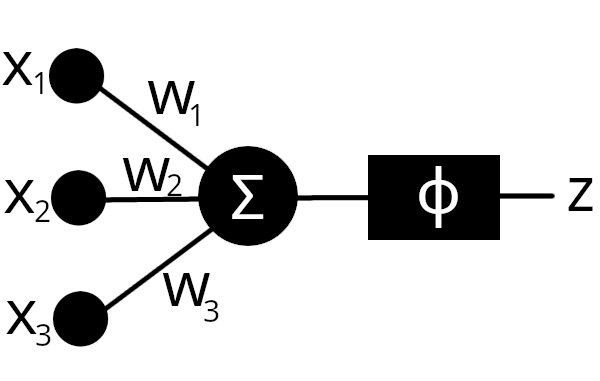
\includegraphics[height=10cm]{figs/Perceptron.png}
    \caption{Perceptron model.}
    \label{fig:perceptron}
\end{figure}

A limitation of the perceptron is that it has limited expressive capabilities, meaning there are some classification problems it is unable to learn. A very simple example is the XOR problem, shown mathematically by \cite{perceptronsbook}. One solution to this limitation was to increase the number of layers, resulting in the Multi-Layered Perceptron (MLP) with increased expressive capabilities.

% Universal approximation theorem?

These types of models are often referred to as feedforward Artificial Neural Networks (ANNs), and can be considered as a type of deep learning model when the number of layers increase. Increasing the layers turns out to give more expressive capabilities in a structured way, where the lower levels learn features of lower abstraction and higher levels learn features of higher abstractions based on the low level abstractions. For example will ANNs trained on images typically learn to detect simple features like edges or certain colors in the lower levels, and then more complex shapes based on these simple features in the higher levels.

At first it was not obvious how to update the weights in lower level layers of the MLP as the weight gradients were not easily computed. With the introduction of the backpropagation algorithm \citep{backprop86} this was again made possible. Backpropagation works by numerically computing gradients based on the chain rule for differentiation. In numerical math, this is usually known as reverse-mode automatic differentiation.

As computing power increased, the number of layers in the ANNs also increased. A problem that arose from training deeper networks is known as the vanishing gradient problem \citep{vanishinggradients}. The problem is simply stated that the gradients of deeper layers tend to zero as the depth increases, making them impossible to train. This leads to overall diminishing returns on increasing network depth. An architecture that attempted to remedy this was residual networks \citep{resnet} which worked by adding skip connections to each layer, thus increasing the effective depth. \cite{resnet} achieved empirically good results on image classification problems with models as deep as 1000 layers using this approach.

%\cite{node} noticed that the forward pass for residual networks had a strong resemblance to the Euler method for numerically solving Ordinary Differential Equations (ODEs). A natural extension to residual networks was then to consider the forward pass in a continuous way, resulting in that the output from the network is now defined by an ODE. This can also be thought of as having infinitely deep neural networks. An advantage of using ODEs is that it makes it possible to leverage the strong theoretical foundations of differential equations and dynamical systems, along with more sophisticated numerical methods for solving the ODEs. \cite{node} designed the architecture called Neural ODE based on this extension, and managed to get particularly good results when learning continuous dynamics or time-series. Neural ODEs also have the advantage of a much lower memory cost compared to residual networks as there are much fewer trainable parameters.

\subsection{Fundamentals}

Machine learning is about algorithms for making a computer automatically learn how to do or accomplish certain tasks. \cite{mitchellmachinelearning} gave the following rigorous definition in his textbook: ``A computer program is said to learn from experience E with respect to some class of tasks T and performance measure P, if its performance at tasks in T, as measured by P, improves with experience E.''

Machine learning is commonly subdivided into the three smaller subjects of supervised learning, unsupervised learning and reinforcement learning. Supervised learning is about problems where the available training data contains both the input data and the corresponding output data, called labels. Classification and regression are common examples of supervised learning. Classification is when each datapoint belongs to a certain discrete class, and the goal is to find a mapping from the input to the correct class. Regression is when the datapoints map to a continuous output and the goal is to find a function which approximates the underlying mapping. Classification can be considered as a discrete version of regression, but will often rely on different machine learning algorithms.


In contrast, unsupervised learning is when the training data only contains the input with no defined output. The goal is not necessarily well-defined either, one possibility can be to look for common patterns in the data to extract some information. Common unsupervised algorithms provide insight into data through clustering or learning other representations and compressing the data in efficient ways. Also note that semi-supervised learning is a thing when only some of the data has labels. Finally, reinforcement learning deals with how to train an agent to interact in an environment to accomplish certain goals. Reinforcement learning can be used for classical control problems such as stabilizing an inverse pendulum or moving a robotic manipulator. Although reinforcement learning is often more useful when it is difficult to find an explicit model of the system, making the algorithms useful for playing board games like chess.

This master project will mainly deal with supervised learning going forwards. The supervised setting starts with a dataset $\mathbb{X} = \{ (\bm{x}^{(1)}, \bm{y}^{(1)}), \dots, (\bm{x}^{(m)}, \bm{y}^{(m)}) \}$ containing $m$ tuples of inputs $\bm{x}^{(i)} \in \mathbb{R}^{n_i}$ and corresponding labels $\bm{y}^{(i)} \in \mathbb{R}^{n_o}$. The goal is to find a function $\bm{f}(\bm{x}; \bm{\theta})$ that maps the input $\bm{x}$ to the output $\bm{y}$, parametrized by $\bm{\theta}$. Different types of $\bm{f}$ functions can be used, and will result in different types of machine learning algorithms called models. The choice of $\bm{f}$ is also dependent on the specific problem to be solved, for example will different models be used for classification as opposed to regression problems. A simple example is the linear function $f(\bm{x}; \bm{\theta}) = \bm{w}^T \bm{x} + b$, with $\bm{\theta} = \begin{bmatrix}\bm{w} \\ b \end{bmatrix}$ that can be used to perform linear regression.

$\bm{f}$ should also be the function that best fits the dataset according to a predefined performance measure. The standard approach is to define an optimization problem with a loss function $\mathcal{L}$ dependent on $f$ and $\mathbb{X}$. The function that optimizes the loss function is then considered to be the best fitting model. An example loss function can be to minimize the Mean Squared Error (MSE), resulting in the loss function $\mathcal{L} = \frac{1}{m} \sum_{i=0}^{m} ||\bm{f}(\bm{x}^{(i)}; \bm{\theta}) - \bm{y}^{(i)}||^2$, often used for simple regression problems. Most optimization problems in the context of machine learning are solved by numerical methods. More details on the optimization process that is relevant for the master project will be elaborated on in the next section.

When the loss function is optimized over the entire dataset it can often lead to a problem known as overfitting. This means that the trained function $\bm{f}$ performs well on the datapoints in the dataset, but performs worse on new datapoints. The goal of machine learning is to train a model on data so that it can generalize the problem and be used for new datapoints. A good way to measure performance is then to split the dataset into both a training and validation set, and calculate the actual performance measure of the model on the validation set while the training set is used for the optimization process. This will give a more accurate performance measure for how the model would work on new never before seen datapoints.

Many datapoints sampled from real life systems will often contain some form of noise which could lead to $\bm{f}$ learning additional information corresponding to the specific noise realization of the dataset. There exist many different techniques for reducing the potential to overfit for different types of models, but the general goal of these techniques is often to reduce the model complexity by limiting the expressive capabilities.

% overfitting figur, lineære datapunkter med noise eksempel

 %more techniques later (regularization, dropout, bachnorm) ?

\subsection{Deep Learning}
\label{sec:deeplearning}

Deep learning is a subfield of machine learning that deals with some specific algorithms and models. Many standard machine learning algorithms are dependent on finding a good way to represent or transform the input data so it is possible to train a model efficiently. Deep learning can be thought of as a method of automatically incorporating representation learning into the models. This works in a structured way by first learning simpler features of low abstraction levels and then combining these features into more and more complex features of higher abstractions \citep{deeplearningbook}. Models usually consist of multiple layers where each layer is responsible for one abstraction level.

The original deep learning models came from the MLP models inspired by the biological neural networks found in brains. A standard feedforward ANN takes the general form:

\begin{equation}
    % multiline: without alignment
    % split: with alignment,
    \begin{split}
        \bm{z}_1 = & \bm{\phi_1}(\bm{W}_1 \bm{x} + \bm{b}_1) \\
        \bm{z}_2 = & \bm{\phi_2}(\bm{W}_1 \bm{z}_1 + \bm{b}_2) \\
        & \vdots \\
        \bm{z}_k = & \bm{\phi_k}(\bm{W}_k \bm{z}_{k-1} + \bm{b}_k) \\
    \end{split}
    \label{eq:ann_forward}
\end{equation}

\noindent where $\bm{x}$ is the input and $\bm{z}_k$ is the output of an ANN with $k$ layers. $\bm{z}_i$ is the output of layer $i$ with $\bm{W}_i$ and $ \bm{b}_i$ as the layer parameters. The matrix $\bm{W}_i$ is called the weights of the layer, and the dimensions are based on the number of neurons in the layer. The vector $\bm{b}$ is called the bias. $\bm{\phi_i}$ is a scalar function evaluated elementwise called the activation function. A nonlinear activation function is necessary for ANNs to be able to approximate any function. Activation functions will often have some form of saturation to reduce numerical errors when the numbers go to $\pm \infty$. The classical go-to was the sigmoid function $\sigma(z) = \frac{1}{1 + e^{-z}}$, but other functions can also be used like the Rectified Linear Unit (ReLU) $g(z) = \max(0, z)$. Sending an input $\bm{x}$ through (\ref{eq:ann_forward}) to get the output $\bm{z}_k$ is called a forward pass.

\begin{figure}[H]
    \centering
    \includesvg[height=10cm]{figs/ann.svg}
    \caption{Example of a simple Artificial Neural Network, represented as a directed graph.}
    \label{fig:ann}
\end{figure}

The number of layers, the amount of neurons in each layer and the choice of activation functions are design variables called hyperparameters, and are usually predetermined before training the model. When training an ANN the goal is to minimize some loss function $\mathcal{L}$. A common approach is to use a gradient-based algorithm to solve this optimization problem. Many sophisticated algorithms exist for this purpose, but a first order gradient descent is the most common due to the usually large amounts of data and number of parameters to optimize for. First order means in this case that we only use the first derivatives for the optimization. The gradient descent algorithms are often replaced with stochastic versions, where training datapoints are randomly sampled from the overall training set and grouped together in a so-called minibatch. If the datapoints are sampled independently, the computed gradient will provide an unbiased estimate of the true gradient \citep{deeplearningbook}. This means that the computed gradients will on average be equal to the true gradient computed over the whole training set.

The gradient vector of any function has the property that it points in the direction of steepest ascent. This also means that the negative of the gradient will then point in the direction of steepest descent. The gradient can then be used to find the local minimum of a loss function by moving along the direction of the negative of the gradient. This leads to the iterative algorithm called Stochastic Gradient Descent (SGD), where the update law is on the following form:

\begin{equation}
    \bm{\theta} \leftarrow \bm{\theta} - \alpha \nabla_{\bm{\theta}} \mathcal{L}
    \label{eq:sgd}
\end{equation}

\begin{figure}[H]
    \centering
    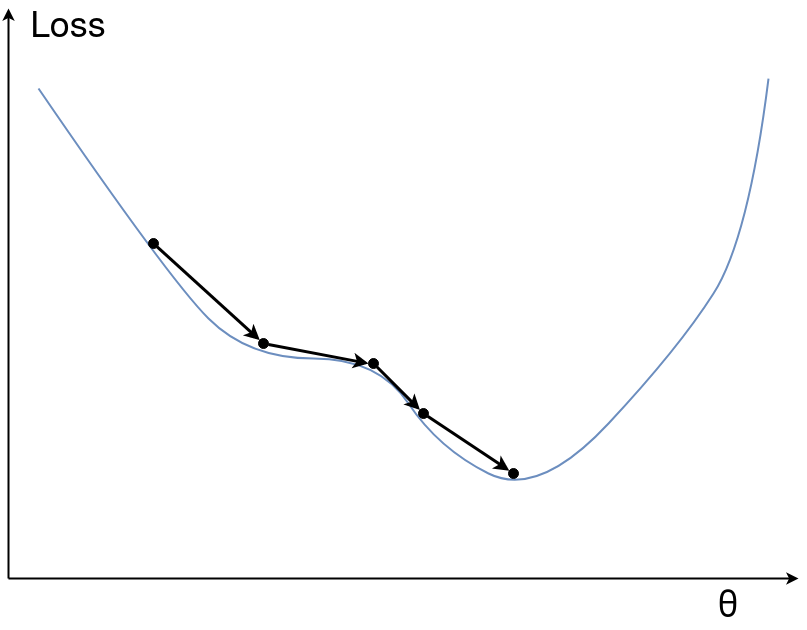
\includegraphics[height=10cm]{figs/gradientdescent.png}
    \caption{Simplified example of how gradient descent minimizes the loss with respect to the parameters $\bm{\theta}$.}
    \label{fig:gradientdescent}
\end{figure}

The parameter vector $\bm{\theta}$ can here be considered as the concatenation of the flattened $\bm{W}_i$ matrices and $\bm{b}_i$ vectors for each layer $i$ in the ANN, but in practice it is easier to calculate the gradient for each parameter vector separately. $\alpha$ is a hyperparameter called the learning rate, and determines the speed of convergence. The SGD algorithm is usually run for a fixed number of iterations called epochs. $\nabla_{\bm{\theta}} \mathcal{L}$ is calculated based on a randomly sampled minibatch of datapoints for each iteration. It is also common to extend SGD with different types of momentum based approaches. Because the loss function landscape is often very rugged and non-convex, momentum can help with escaping local minimas and speed up convergence. A decaying learning rate is also often used to ensure convergence with stochastic gradients.

\begin{figure}[H]
    \centering
    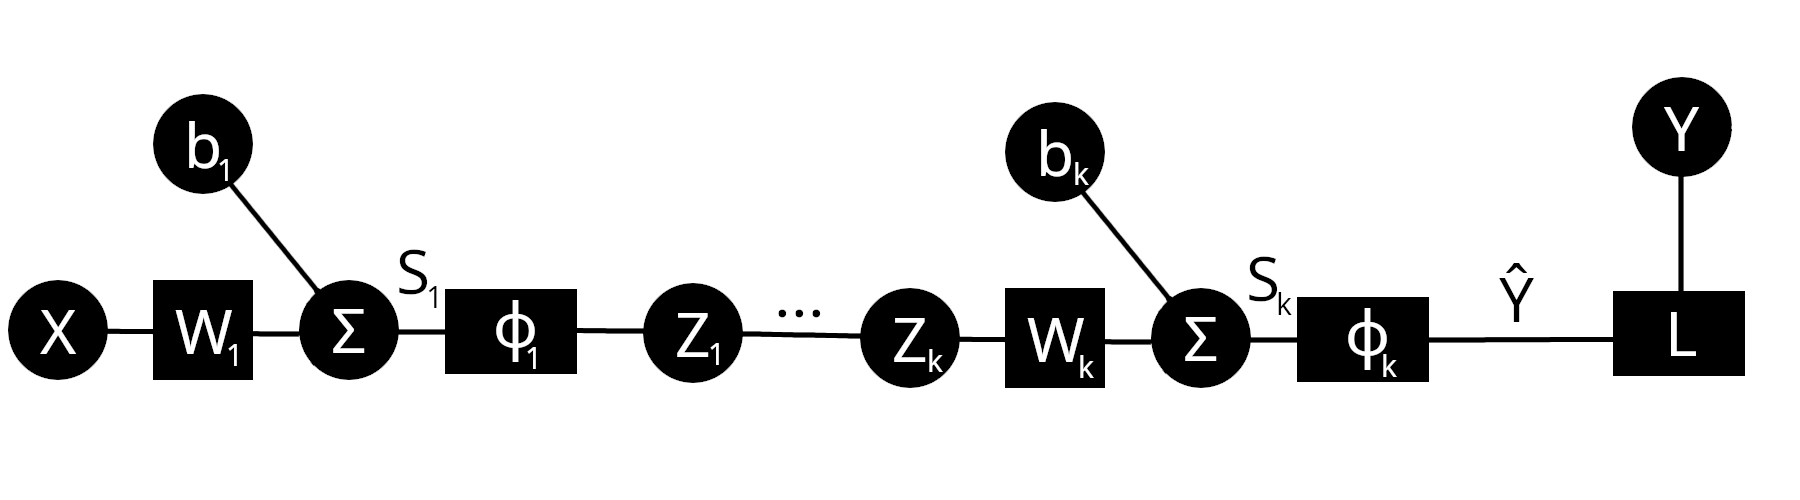
\includegraphics[height=5cm]{figs/deepnetwork.png}
    \caption{Deep Neural Network.}
    \label{fig:deepnetwork}
\end{figure}

Calculating gradients of the loss function with respect to the ANN parameters $\nabla_{\bm{\theta}} \mathcal{L}$ requires the use of the backpropagation algorithm. To simplify notation, write $\nabla_{\bm{\theta}} \mathcal{L} = \frac{\partial \mathcal{L}}{\partial \bm{\theta}}$. Backpropagation is based on the chain rule of derivatives from calculus. Expand the term as a product of multiple gradients and jacobians:

\begin{equation}
    \frac{\partial \mathcal{L}}{\partial \bm{\theta}_k}
    = \frac{\partial \mathcal{L}}{\partial \bm{z}_k} \frac{\partial \bm{z}_k}{\partial \bm{\theta}_k}
    = \frac{\partial \mathcal{L}}{\partial \bm{z}_k} \frac{\partial \bm{\phi}_k}{\partial \bm{s}_k} \frac{\partial \bm{s}_k}{\partial \bm{\theta}_k}
\end{equation}

\noindent where $\bm{s}_k = \bm{W}_k \bm{z}_{k-1} + \bm{b}_k$. All the factors can be considered well-defined and easily computable analytically. This procedure will get the gradients to the output layer $k$ of the ANN. To get gradients to previous layers, more applications of the chain rule are necessary:

\begin{equation}
    \frac{\partial \mathcal{L}}{\partial \bm{\theta}_{k-1}}
    = \frac{\partial \mathcal{L}}{\partial \bm{z}_k} \frac{\partial \bm{\phi}_k}{\partial \bm{s}_k} \frac{\partial \bm{s}_k}{\partial \bm{z}_{k-1}} \frac{\partial \bm{z}_{k-1}}{\partial \bm{\theta}_{k-1}}
    = \frac{\partial \mathcal{L}}{\partial \bm{z}_k} \frac{\partial \bm{\phi}_k}{\partial \bm{s}_k} \frac{\partial \bm{s}_k}{\partial \bm{z}_{k-1}} \frac{\partial \bm{\phi}_{k-1}}{\partial \bm{s}_{k-1}} \frac{\partial \bm{s}_{k-1}}{\partial \bm{\theta}_{k-1}}
\end{equation}

This generalizes to the recursive formula:

\begin{equation}
    \frac{\partial \mathcal{L}}{\partial \bm{\theta}_{i}}
    = \frac{\partial \mathcal{L}}{\partial \bm{z}_k} \frac{\partial \bm{z}_k}{\partial \bm{z}_{k-1}} \dots \frac{\partial \bm{z}_{i+1}}{\partial \bm{z}_i} \frac{\partial \bm{z}_i}{\partial \bm{\theta}_i}
\label{eq:backprop}
\end{equation}

\noindent with

\begin{equation}
\begin{aligned}[t]
    \frac{\partial \bm{z}_{i+1}}{\partial \bm{z}_i}
    = \frac{\partial \bm{\phi}_{i+1}}{\partial \bm{s}_{i+1}} \frac{\partial \bm{s}_{i+1}}{\partial \bm{z}_i}
\end{aligned}
\qquad
\qquad
\qquad
\begin{aligned}[t]
    \frac{\partial \bm{z}_i}{\partial \bm{\theta}_i}
    = \frac{\partial \bm{\phi}_i}{\partial \bm{s}_i} \frac{\partial \bm{s}_i}{\partial \bm{\theta}_i}
\end{aligned}
\end{equation}

\noindent which gives the complete backpropagation algorithm. Computing the gradients in this way is called to do a backward pass of the ANN.

When training ANNs the gradients have a tendency to eventually become small, and when many of these small gradients are multiplied together they will usually vanish at deeper layers, meaning they approach zero. This causes the parameters of the deeper layers to change very little by training, and leads to an overall lower network performance than what could theoretically be achieved. This is known as the vanishing gradient problem.

Residual Networks is a neural network architecture that attempts to remedy this problem. The architecture works by adding skip connections in between layer outputs. This causes the backpropagation pathway from the output to the input to effectively be much shorter, thus allowing gradients to flow easier backwards. Skip connections can be added to any type of neural network, but for a standard feedforward network the forward pass would take the form:

\begin{equation}
    \begin{split}
        \bm{z}_1 = & \bm{x} + \bm{\phi_1}(\bm{W}_1 \bm{x} + \bm{b}_1) \\
        \bm{z}_2 = & \bm{z}_1 + \bm{\phi_2}(\bm{W}_1 \bm{z}_1 + \bm{b}_2) \\
        & \vdots \\
        \bm{z}_k = & \bm{z}_{k-1} + \bm{\phi_k}(\bm{W}_k \bm{z}_{k-1} + \bm{b}_k) \\
    \end{split}
    \label{eq:resnet_forward}
\end{equation}

Finally, it is also worth noting that there exists other model architectures. Some examples include Convolutional Neural Networks (CNNs) and Recurrent Neural Networks (RNNs). Both of these architectures have their own ways of doing the forward and backward pass, but are still based on the same principles as feedforward networks since gradients from the loss function to the parameters are required. CNNs are based on the convolution operator commonly used in signal processing applications. Because of the translation-invariance of convolutions, CNNs often work well on data with translation-invariant features. An example of this are objects in images, as the type of object is not dependent on the position of the object within the image. RNNs are based on having temporal connections in the data. This makes them particularly useful for data with sequential patterns like text or time-series.

%RNNs define a TODO

Neural ODEs, the main focus of this thesis, is another type of neural network architecture. The forward and backward pass will be explained in detail later on.

\section{Ordinary Differential Equations}

\subsection{Introduction}

Many things related to physics, biology, economics and engineering can be considered as a dynamical system. This means that there are one or more state variables which change over time defined by a set of rules. Differential equations are a useful mathematical tool for modeling the behavior of a dynamical system when the state variables change in continuous time.

In the most general version, a differential equation is an equation that involves one or more independent variables, one or more state variables that depend on the independent variables and some of their derivatives of any order. When there are only one independent variable, for example time, the result is an Ordinary Differential Equation (ODE). Multiple independent variables result in a Partial Differential Equation (PDE). Only ODEs will be considered in this thesis.

ODEs are generally expressed on the explicit form:

\begin{equation}
    \dot{\bm{x}} = \bm{f}(t, \bm{x})
    \label{eq:ode}
\end{equation}

\noindent with $t$ as the independent variable, $\bm{x}(t)$ as the state vector, $\dot{\bm{x}} = \frac{d \bm{x}}{d t}$ and a vector field $\bm{f}(t, \bm{x})$. ODEs can also be defined implicitly as $\bm{F}(t, \bm{x}, \dot{\bm{x}}) = \bm{0}$, but are usually less practical to work with.

ODEs with higher order derivatives can always be transformed into the form (\ref{eq:ode}) by simply augmenting the state vector. Consider the scalar ODE $\frac{d^2 x}{d t^2} = f(t, x)$ as an example. Start by defining $x_1 = x$ and $x_2 = \dot{x}$. Then $\dot{x_1} = x_2$ and $\dot{x_2} = f(t, x_1)$, which looks like $\frac{d}{d t} \begin{bmatrix} x_1 \\ x_2 \end{bmatrix} = \begin{bmatrix} x_2 \\ f(t, x_1) \end{bmatrix}$ when written on the form of (\ref{eq:ode}). This also means that the order of an ODE is equivalent to the number of state variables.

An ODE that does not explicitly depend on the independent variable is called autonomous. It can then be written in the form $\dot{\bm{x}} = \bm{f}(\bm{x})$. If the ODE does explicitly depend on the independent variable it is called non-autonomous.

As an ODE only defines the rate of change there can be many different functions that satisfy the equation. An Initial Value Problem (IVP) is defined as an ODE of the form (\ref{eq:ode}) with the addition of an initial value $\bm{x}(t_0) = \bm{x}_0$. According to the Picard-Lindelöf theorem \citep{kreyszigfunctional} an IVP has a unique solution if $\bm{f}(t, \bm{x})$ is Lipschitz continuous in $\bm{x}$ and continuous in $t$. A function $\bm{f}$ is defined to be Lipschitz continuous if there exists a  $k>0$ such that $||\bm{f}(\bm{x}) - \bm{f}(\bm{y})|| \leq k ||\bm{x} - \bm{y}||$. If a function is continuous and also has continuous first order derivatives, it implies that the function is Lipschitz continuous.

The solution of an IVP at time $t_1$ can be found by integrating the ODE from the initial value at $t_0$:

\begin{equation}
    \bm{x}(t_1) = \bm{x}(t_0) + \int_{t_0}^{t_1} \bm{f}(t, \bm{x}(t)) dt
    \label{eq:ode_solution}
\end{equation}

\subsection{Numerical Methods}
\label{sec:numericalmethods}

Even though an IVP has a unique solution it does not mean that the solution has a closed-form expression which can be found analytically. This is the case for most IVPs, so there has been developed many methods for numerically solving the IVP instead.

Euler's method is one of the earliest and simplest methods. It is an iterative algorithm based on an approximation of the derivative. To derive the method start with the definition of the derivative:

\begin{equation}
    \dot{\bm{x}} = \frac{d \bm{x}}{d t} = \lim_{h \rightarrow 0} \frac{\bm{x}(t + h) - \bm{x}(t)}{h}
    \label{eq:derivative}
\end{equation}

If h is set to a small value, the expression inside the limit of (\ref{eq:derivative}) will work as an approximation of the derivative and can be inserted into (\ref{eq:ode}) to get:

\begin{equation*}
    \frac{\bm{x}(t + h) - \bm{x}(t)}{h} = \bm{f}(t, \bm{x})
\end{equation*}

\begin{equation*}
    \bm{x}(t + h) = \bm{x}(t) + h \bm{f}(t, \bm{x}(t))
\end{equation*}

\noindent which gives the iterative algorithm:

\begin{equation}
    \begin{split}
        \bm{x}_{n+1} &= \bm{x}_n + h \bm{f}(t_n, \bm{x}_n) \\
        t_{n+1} &= t_n + h
    \end{split}
    \label{eq:euler}
\end{equation}

The algorithm based on (\ref{eq:euler}) can then be iterated until the desired end time is reached as $n = \frac{t_{\textrm{end}}}{h}$ to get the final output. Iterating an ODE in such a manner is also called to integrate it. A problem with the Euler method is that because it is a first order integrator it will generally start to deviate from the true IVP solution. More specifically, the global error is linear in the step size.

Runge-Kutta methods are a generalization of the Euler method that improves the global error of the integration. They do this by increasing the amount of stages per iteration, and thus also the order of the integrator. To see how this works, consider the example of the commonly used fourth order explicit Runge-Kutta method RK4:

\begin{equation}
    \begin{split}
        \bm{k_1} &= \bm{f}(t_n, \bm{x}_n) \\
        \bm{k_2} &= \bm{f}(t_n + \frac{h}{2}, \bm{x}_n + h \frac{\bm{k_1}}{2}) \\
        \bm{k_3} &= \bm{f}(t_n + \frac{h}{2}, \bm{x}_n + h \frac{\bm{k_2}}{2}) \\
        \bm{k_4} &= \bm{f}(t_n + h, \bm{x}_n + h \bm{k_3}) \\
        \bm{x}_{n+1} &= \bm{x}_n + \frac{1}{6} h (\bm{k_1} + 2 \bm{k_2} + 2 \bm{k_3} + \bm{k_4}) \\
        t_{n+1} &= t_n + h
    \end{split}
    \label{eq:rk4}
\end{equation}

As the true trajectory is approximated closer by averaging midpoints, RK4 manages to achieve a much smaller global error, which means that the numerical trajectory will follow the true trajectory closer and for a longer time.

Runge-Kutta methods can in general be described by what is known as Butcher tableaus. The Butcher tableau of RK4 based on the coefficients of (\ref{eq:rk4}) is:

\renewcommand\arraystretch{1.2}
\begin{equation}
    \begin{array}
    {c|cccc}
    0\\
    \frac{1}{2} & \frac{1}{2}\\
    \frac{1}{2} &0 &\frac{1}{2} \\
    1& 0& 0& 1\\
    \hline
    & \frac{1}{6} &\frac{1}{3} &\frac{1}{3} &\frac{1}{6} 
    \end{array}
    \label{eq:rk4_butcher}
\end{equation}

General Butcher tableaus take the form:

\begin{equation}
    \begin{array}
    {c|cccc}
    c_1 & a_{11} & a_{12} & \dots & a_{1s} \\
    c_2 & a_{21} & a_{22} & \dots & a_{2s} \\
    \vdots & \vdots & \vdots & \ddots & \vdots \\
    c_s & a_{s1} & a_{s2} & \dots & a_{ss} \\
    \hline
    & b_1 & b_2 & \dots & b_s
    \end{array}
    \label{eq:butcher}
\end{equation}

and are applied to the general Runge-Kutta method in the following way:

\begin{equation}
    \begin{split}
        \bm{k}_1 &= \bm{f}(t_n + c_1 h, \bm{x}_n + h \sum_{j=1}^{s} a_{1j} \bm{k}_j) \\
        \bm{k}_2 &= \bm{f}(t_n + c_2 h, \bm{x}_n + h \sum_{j=1}^{s} a_{2j} \bm{k}_j) \\
        \vdots \\
        \bm{k}_s &= \bm{f}(t_n + c_s h, \bm{x}_n + h \sum_{j=1}^{s} a_{sj} \bm{k}_j) \\
        \bm{x}_{n+1} &= \bm{x}_n + h \sum_{i=1}^{s} b_i \bm{k}_i \\
        t_{n+1} &= t_n + h
    \end{split}
\end{equation}

When the upper triangular $a$ values in the Butcher tableau (\ref{eq:butcher}) are zero (or omitted as in the RK4 Butcher tableau (\ref{eq:rk4_butcher})) the resulting Runge-Kutta method is called explicit. Explicit methods can be solved by iteratively calculating the $k$ values. When the upper triangular $a$ values are nonzero, the Runge-Kutta method is implicit and requires the solution of a nonlinear set of equations to calculate all the $k$ values. This can for example be done with Newton's method, which is an iterative method for solving nonlinear equations. Without explaining all the details, Newton's method solves equations of the form $\bm{x} = \bm{f}(\bm{x})$ with iterations $\bm{x}_{n+1} = \bm{x}_n - (\frac{\partial \bm{f}}{\partial \bm{x}})^{-1} \bm{f}(\bm{x}_n)$. Implicit methods will often have higher orders for a fewer number of stages, but come with the disadvantage of being more expensive to compute because of the Newton iterations.

Another common Runge-Kutta scheme is the Dormand-Prince method \citep{dopri}, which is commonly used commercially. It is an explicit method with seven stages. It also calculates both the fourth and fifth order errors which makes it possible to automatically change the step size $h$ of the integrator. When the ODE has many rapid changes it is best to use a small step size to ensure that the trajectory is accurately followed, and when the ODE is relatively flat it could be a good idea to speed up the integration by increasing the step size. The Dormand-Prince method can therefore be used as an adaptive step size integrator.

\section{Neural ODEs}
\label{sec:node}

Neural ODEs came from the realization that the equation for the forward pass of Residual Networks (\ref{eq:resnet_forward}) has a strong resemblance to the equation for the Euler method of integration (\ref{eq:euler}). The main differences are that the step size $h$ is set to $1$ for Residual Networks, and that the Residual Networks can have different functions for each iteration.

\begin{figure}[H]
    \centering
    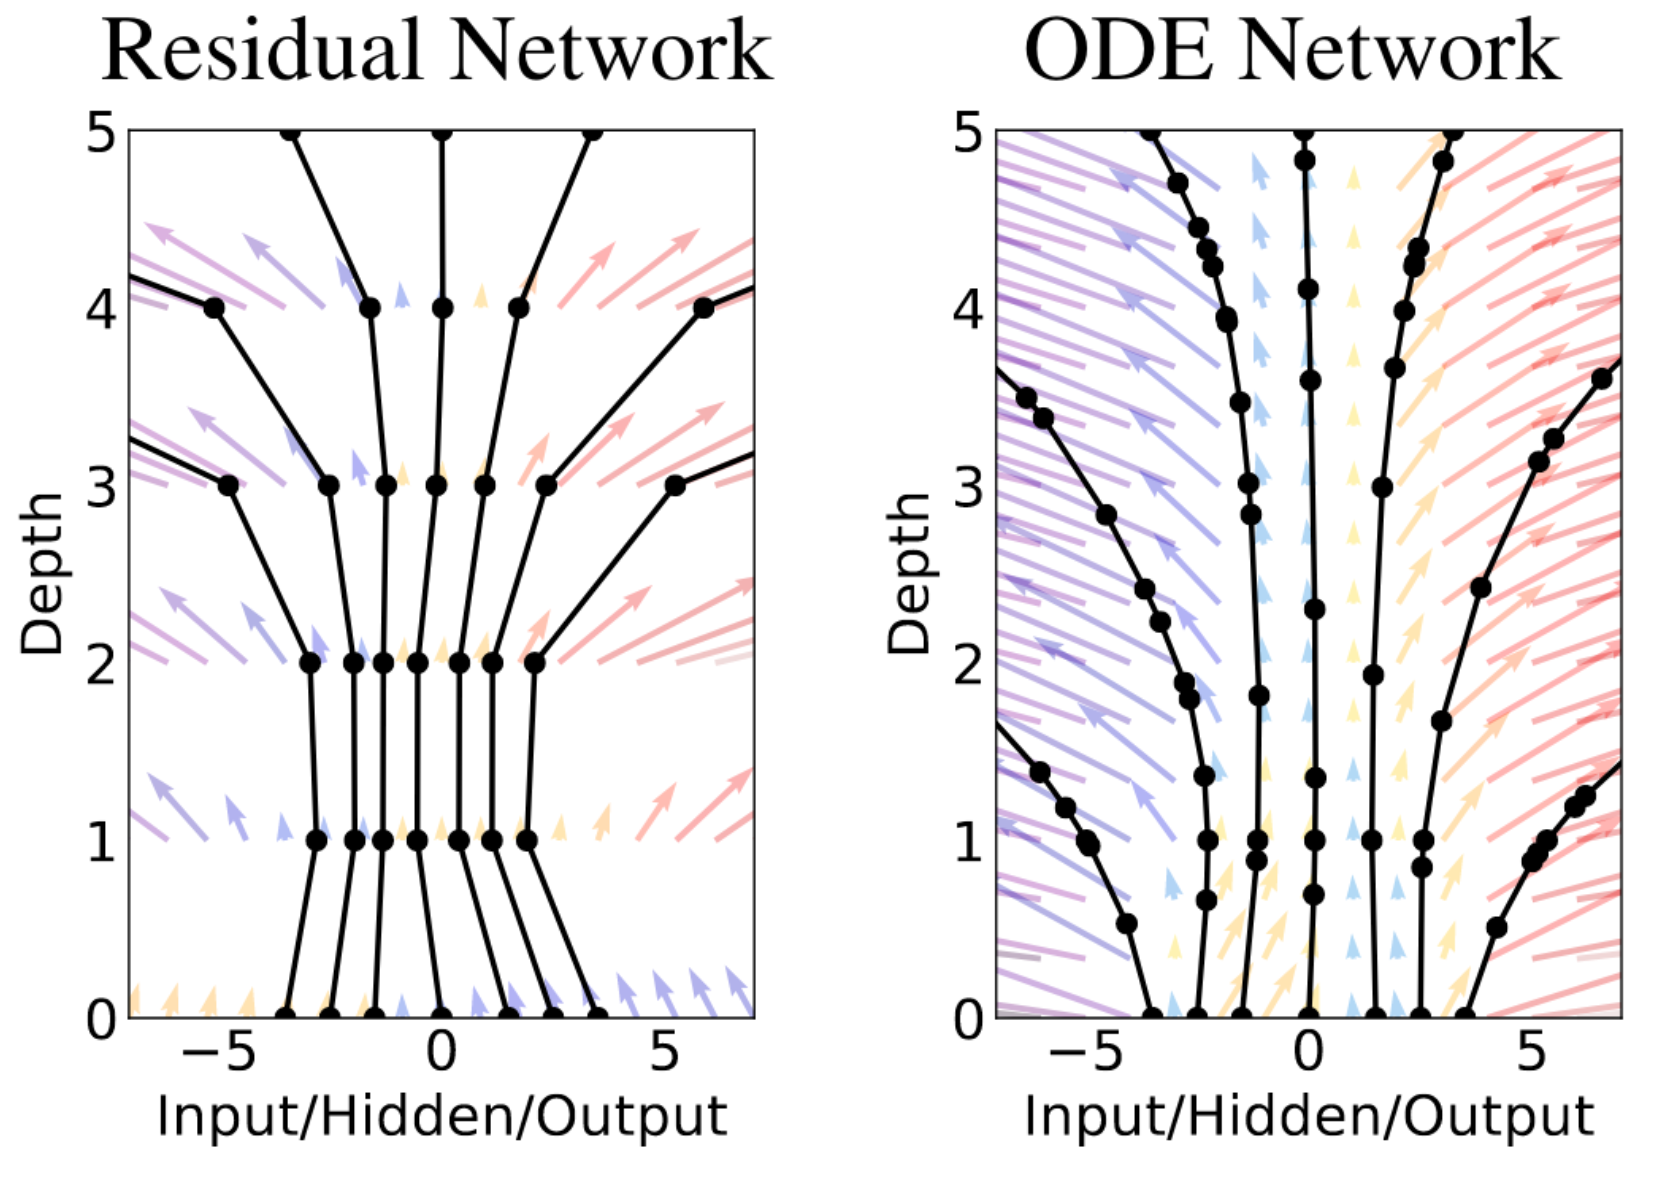
\includegraphics[height=10cm]{figs/resnetlimit.png}
    \caption{Left: Residual Network with discrete steps. Right: Neural ODE with continuous steps. Figure taken from \cite{node}.}
    \label{fig:resnetlimit}
\end{figure}

The idea was then to extend Residual Networks by designing a neural network defined by an ODE, and then leveraging more sophisticated methods of numerical integration. Neural ODEs can be defined with the structure:

\begin{equation}
    \dot{\bm{x}} = \bm{f}(t, \bm{x}; \bm{\theta})
    \label{eq:node_structure}
\end{equation}

\noindent where $\bm{f}$ is a function parametrized by $\bm{\theta}$. For example could $\bm{f}$ be defined as another neural network, which may or may not depend on the independent variable $t$. Because $\bm{x}$ is now assumed to follow a trajectory in continuous time, this is effectively the same as thinking of a residual network with infinite depth. For a given initial condition $\bm{x}(t_0)$, the solution of (\ref{eq:node_structure}) can be written on the form:

\begin{equation}
    \bm{x}(t_1) = \bm{x}(t_0) + \int_{t_0}^{t_1} \bm{f}(t, \bm{x}(t) ; \bm{\theta}) dt
    \label{eq:node_forward}
\end{equation}

\noindent which defines the forward pass of the Neural ODE architecture when the initial condition $\bm{x}(t_0)$ is considered as the input to the network, and $\bm{x}(t_1)$ is considered as the output. Neural networks are Lipschitz continuous by construction, which means that the Picard-Lindelöf theorem ensures the existence and uniqueness of the output.

The integration limits $t_0$ and $t_1$ can either be considered as a part of the training data, or as hyperparameters for the network when the time is irrelevant. This is often the case when training Neural ODEs for the purpose of feature representations. Also setting $t_0 = 0$ if possible can often lead to a simplified training process. One noteworthy limitation of the architecture is that the input and output dimensions must be equal. (\ref{eq:node_forward}) can then be integrated with any numerical integration method.

Training a Neural ODE model is done similarly to other deep learning models. This means defining a loss function $\mathcal{L}$ to minimize over a training dataset. Datapoints will consist of an input value $\bm{x}(t_0)$ and one or more output values $\bm{x}(t_i)$ for a given set of time values $t_i$. One datapoint can then be either an input-output pair, or a full time-series trajectory depending on the application. The goal is now to find the parametrizable function $\bm{f}(t, \bm{x}; \bm{\theta})$ such that the outputs $\bm{x}(t_1)$ defined by equation (\ref{eq:node_forward}) minimize $\mathcal{L}$ for all $t_1 = t_i$.

To solve this minimization problem it is necessary to compute gradients from the loss function $\mathcal{L}$ to the parameters $\bm{\theta}$ of $\bm{f}$, meaning $\frac{\partial \mathcal{L}}{\partial \bm{\theta}}$. All the operations of a numerical integrator are differentiable so it is in theory possible to keep track of all operations during the forward pass, and compute the gradients through automatic differentiation. This is in general very memory intensive and could also use a variable amount of memory with adaptive step size solvers. Overall, this approach is not practical for any larger networks or real datasets.

\cite{node} used what is called the adjoint sensitivity method \citep{pontryagin62} to compute the gradients in a novel way. Start by defining what is called the adjoint state:

\begin{equation}
    \bm{a}(t) = \frac{\partial \mathcal{L}}{\partial \bm{x}(t)}
\end{equation}

It can be shown that the adjoint has another equivalent definition based on an ODE \citep{node}. To see this, start by rewriting the adjoint by applying the chain rule:

\begin{equation*}
    \bm{a}(t) = \frac{\partial \mathcal{L}}{\partial \bm{x}(t)} = \frac{\partial \mathcal{L}}{\partial \bm{x}(t + h)} \frac{\partial \bm{x}(t+h)}{\partial \bm{x}(t)} = \bm{a}(t+h) \frac{\partial \bm{x}(t+h)}{\partial \bm{x}(t)}
\end{equation*}

The new variable $h$ signifies a small step in $t$. Now derive the ODE by using the definition of the derivative together with the previously found expression:

\begin{equation*}
    \frac{d \bm{a}(t)}{d t} = \lim_{h \rightarrow 0} \frac{\bm{a}(t + h) - \bm{a}(t)}{h}
    = \lim_{h \rightarrow 0} \frac{\bm{a}(t + h) - \bm{a}(t+h) \frac{\partial \bm{x}(t+h)}{\partial \bm{x}(t)}}{h}
\end{equation*}

Then do a taylor expansion of the term $\bm{x}(t+h) = \bm{x}(t) + h \dot{\bm{x}} + \mathcal{O}(h^2) = \bm{x}(t) + h \bm{f}(t, \bm{x}; \bm{\theta}) + \mathcal{O}(h^2)$ and insert into the expression:

\begin{equation*}
    \frac{d \bm{a}(t)}{d t} = \lim_{h \rightarrow 0} \frac{\bm{a}(t + h) - \bm{a}(t+h) \frac{\partial}{\partial \bm{x}(t)}(\bm{x}(t) + h \bm{f}(t, \bm{x}; \bm{\theta}) + \mathcal{O}(h^2))}{h}
\end{equation*}

\begin{equation*}
    \frac{d \bm{a}(t)}{d t} = \lim_{h \rightarrow 0} \frac{\bm{a}(t + h) - \bm{a}(t+h) (I + h \frac{\partial \bm{f}(t, \bm{x}; \bm{\theta})}{\partial \bm{x}(t)} + \mathcal{O}(h^2))}{h}
\end{equation*}

\begin{equation*}
    \frac{d \bm{a}(t)}{d t} = \lim_{h \rightarrow 0} \frac{- h \bm{a}(t+h) \frac{\partial \bm{f}(t, \bm{x}; \bm{\theta})}{\partial \bm{x}(t)} + \mathcal{O}(h^2)}{h}
\end{equation*}

\begin{equation*}
    \frac{d \bm{a}(t)}{d t} = \lim_{h \rightarrow 0} - \bm{a}(t+h) \frac{\partial \bm{f}(t, \bm{x}; \bm{\theta})}{\partial \bm{x}(t)} + \mathcal{O}(h)
\end{equation*}

\begin{equation}
    \frac{d \bm{a}(t)}{d t} = - \bm{a}(t) \frac{\partial \bm{f}(t, \bm{x}(t) ; \bm{\theta})}{\partial \bm{x}}
\label{eq:adjoint_ode}
\end{equation}

This ODE can be solved in the same way as (\ref{eq:ode_solution}) for a given initial value $\bm{a}(t_1)$ by integrating from $t_1$ to $t_0$:

\begin{equation}
    \bm{a}(t_0) = \bm{a}(t_1) + \int_{t_1}^{t_0} - \bm{a}(t) \frac{\partial \bm{f}(t, \bm{x}(t) ; \bm{\theta})}{\partial \bm{x}} dt
\label{eq:adjoint_ode_solution}
\end{equation}

In this context, $\bm{x}(t_1)$ is the output from the Neural ODE and the initial value $\bm{a}(t_1) = \frac{\partial \mathcal{L}}{\partial \bm{x}(t_1)}$ can be considered to already be given from the loss function directly, or computed from the backpropagation algorithm (\ref{eq:backprop}) if there are more neural network layers after the Neural ODE and before the loss function. Solving (\ref{eq:adjoint_ode_solution}) results in $\bm{a}(t_0) = \frac{\partial \mathcal{L}}{\partial \bm{x}(t_0)}$ which is the gradients from the loss function $\mathcal{L}$ to the input $\bm{x}(t_0)$ of the Neural ODE. This gradient is necessary in order to continue the backpropagation algorithm to deeper layers.

The gradient to the parameters $\frac{\partial \mathcal{L}}{\partial \bm{\theta}}$ is still needed to solve the optimization problem. To derive an expression, start by defining an augmented adjoint $\bm{a}_{\textrm{aug}} = \begin{bmatrix} \frac{\partial \mathcal{L}}{\partial \bm{x}} & \frac{\partial \mathcal{L}}{\partial \bm{\theta}} \end{bmatrix}$. Using the same reasoning for deriving adjoint ODE (\ref{eq:adjoint_ode}) results in the following expression for the time derivative of the augmented adjoint:

\begin{equation*}
    \frac{d \bm{a}_{\textrm{aug}}}{d t}
    = - \begin{bmatrix} \frac{\partial \mathcal{L}}{\partial \bm{x}} & \frac{\partial \mathcal{L}}{\partial \bm{\theta}} \end{bmatrix} \begin{bmatrix} \frac{\partial}{\partial \bm{x}} \frac{d \bm{x}}{d t} & \frac{\partial}{\partial \bm{\theta}} \frac{d \bm{x}}{d t} \\ \frac{\partial}{\partial \bm{x}} \frac{d \bm{\theta}}{d t} & \frac{\partial}{\partial \bm{\theta}} \frac{d \bm{\theta}}{d t} \end{bmatrix}
    = - \begin{bmatrix} \frac{\partial \mathcal{L}}{\partial \bm{x}} & \frac{\partial \mathcal{L}}{\partial \bm{\theta}} \end{bmatrix} \begin{bmatrix} \frac{\partial}{\partial \bm{x}} \bm{f} & \frac{\partial}{\partial \bm{\theta}} \bm{f} \\ \frac{\partial}{\partial \bm{x}} \bm{0} & \frac{\partial}{\partial \bm{\theta}} \bm{0} \end{bmatrix}
\end{equation*}

\noindent with $\frac{d \bm{x}}{d t} = \dot{\bm{x}} = \bm{f}$ and where the zeros in the bottom row appear because $\frac{d \bm{\theta}}{d t} = \bm{0}$. Then multiply the vector with the matrix to get the following:

\begin{equation*}
    \frac{d \bm{a}_{\textrm{aug}}}{d t}
    = \begin{bmatrix} \frac{\partial \mathcal{L}}{\partial \bm{x}} \frac{\partial \bm{f}}{\partial \bm{x}} & \frac{\partial \mathcal{L}}{\partial \bm{x}} \frac{\partial \bm{f}}{\partial \bm{\theta}} \end{bmatrix}
    = \begin{bmatrix} \bm{a}(t) \frac{\partial \bm{f}}{\partial \bm{x}} & \bm{a}(t) \frac{\partial \bm{f}}{\partial \bm{\theta}} \end{bmatrix}
\end{equation*}

Because $\frac{d \bm{a}_{\textrm{aug}}}{d t} = \begin{bmatrix} \frac{d}{d t} \frac{\partial \mathcal{L}}{\partial \bm{x}} & \frac{d}{d t}\frac{\partial \mathcal{L}}{\partial \bm{\theta}} \end{bmatrix}$, this results in the ODE: 

\begin{equation*}
    \frac{d}{d t} \frac{\partial \mathcal{L}}{\partial \bm{\theta}} =  - \bm{a}(t) \frac{\partial \bm{f}(t, \bm{x}(t); \bm{\theta})}{\partial \bm{\theta}}
\end{equation*}

\noindent which can be integrated from $t_1$ to $t_0$ for an expression of the gradients to the parameters $\bm{\theta}$:

\begin{equation}
    \frac{\partial \mathcal{L}}{\partial \bm{\theta}} = \int_{t_1}^{t_0} - \bm{a}(t) \frac{\partial \bm{f}(t, \bm{x}(t) ; \bm{\theta})}{\partial \bm{\theta}} dt
    \label{eq:adjoint_param_integral}
\end{equation}

\noindent with the assumption that the initial value is $\bm{0}$.

Knowing the values of $\bm{x}(t)$ for of $t_0 < t < t_1$ is also required to integrate (\ref{eq:adjoint_param_integral}). Storing the $\bm{x}$ values during the forward pass would not work as the ODE solver running backwards is not guaranteed to use the $\bm{x}$ values at the same points in time. Storing enough $\bm{x}$ values and selecting the one that is the closest to the desired one is something that could work, but will give lower accuracy and higher memory usage. A way of getting the correct $\bm{x}(t)$ values is to simply recompute them by integrating backwards from $\bm{x}(t_1)$ as obtained from the forward pass:

\begin{equation}
    \bm{x}(t_0) = \bm{x}(t_1) + \int_{t_1}^{t_0} \bm{f}(t, \bm{x}(t) ; \bm{\theta}) dt
\end{equation}

There is now a total of three integrals to compute to get $\frac{\partial \mathcal{L}}{\partial \bm{\theta}}$ and $\frac{\partial \mathcal{L}}{\partial \bm{x}(t_0)}$. These integrals can be augmented into one single integral and then solved with one pass to the numerical solver:

\begin{equation}
    \begin{bmatrix}
    \bm{x}(t_0) \\
    \frac{\partial \mathcal{L}}{\partial \bm{x}(t_0)} \\
    \frac{\partial \mathcal{L}}{\partial \bm{\theta}}
    \end{bmatrix} = \begin{bmatrix}
    \bm{x}(t_1) \\
    \frac{\partial \mathcal{L}}{\partial \bm{x}(t_1)} \\
    \bm{0}
    \end{bmatrix} + \int_{t_1}^{t_0} \begin{bmatrix}
    \bm{f}(t, \bm{x}(t) ; \bm{\theta}) \\
    - \bm{a}(t) \frac{\partial \bm{f}(t, \bm{x}(t) ; \bm{\theta})}{\partial \bm{x}} \\
    - \bm{a}(t) \frac{\partial \bm{f}(t, \bm{x}(t) ; \bm{\theta})}{\partial \bm{\theta}}
    \end{bmatrix} dt
    \label{eq:node_backward}
\end{equation}

Finally, note that the jacobian matrices $\frac{\partial \bm{f}(t, \bm{x}(t) ; \bm{\theta})}{\partial \bm{x}}$ and $\frac{\partial \bm{f}(t, \bm{x}(t) ; \bm{\theta})}{\partial \bm{\theta}}$ are also required, but can easily be computed if $\bm{f}$ is defined as a neural network. (\ref{eq:node_backward}) now defines the full backward pass of Neural ODEs.

\cite{resnetlimitnode} later formally proved that the limit of training a Residual Network with the same function in each layer converges to the same loss and gradient values when the that would have been obtained when training a Neural ODE model.

An alternative derivation using concepts from optimal control theory is described in Appendix \ref{appendix:optimalcontroladjoints}.

\chapter{State of the Art}
\label{cha:sota}

Starts with a description of the literature review protocol to showcase how the state of the art was determined. Then goes on to describe the relevant development regarding improvements and modifications to the basic Neural ODE architecture.

\section{Structured Literature Review Protocol}

The first paper read was the original by \cite{node}.

Afterwards, \href{https://www.scinapse.io/}{\color{cyan}{Scinapse}} was used to search for research papers. The original paper was then found on the website along with all citations of that paper. Then these papers were sorted by citations themselves and the first ten pages were browsed through manually.

For each entry the title was read to determine if it could be relevant. If it was of any potential relevance, the abstract was then read to filter even further. This produced a list of papers.

Then a search on both the terms \textit{neural ordinary differential equations} and \textit{neural ode} was done, also on \href{https://www.scinapse.io/}{\color{cyan}{Scinapse}}. The papers searched were from all journals and conferences and chosen to be max five years old. The first five pages of entries were then determined in the same method as above. Not surprisingly there was a lot of overlap with the previous search method.

After this, \href{https://scholar.google.com/}{\color{cyan}{Google Scholar}} was used with the same two search terms as above and filtered for papers newer than one year old. This was done to find the most recent papers without many citations. It is possible that there exists some relevant papers older than one year with too few citations to have shown up yet, but that is very unlikely.

These three steps combined produced a list of papers which were read. Some of the most relevant papers are described in the next sections.

\section{Neural ODE with Extensions}

The original paper by \cite{node} described a new neural network architecture derived from taking the limit of a residual network. The forward and backward pass of this architecture was described thoroughly in section \ref{sec:node}. They managed to achieve an algorithm for the backward pass running in $\mathcal{O}(1)$ memory / space complexity, which allows the Neural ODE to be used for practical applications. For image classification on the MNIST dataset they managed to achieve a test error on par with a residual network using only a third of the parameters, while also training on constant memory. Neural ODEs are in this case used for representation learning equivalent to a deep network, instead of learning a dynamical system.

\cite{node} also realized that the residual forward pass (equation \ref{eq:resnet_forward}) also appears in normalizing flows \citep{normalizingflows}, which is a method for approximating probability distributions for generative models. They then created a continuous version of normalizing flows that managed to achieve slightly better performance than the standard normalizing flows. An additional property they discovered were that the reverse transformation of a normalizing flow is much cheaper to compute with the continuous version, which means that maximum likelihood estimation is a feasible training method. The evolution of the flows from the continuous normalizing flows were also more interpretable than the evolution of the standard normalizing flows.

Another application found was regarding irregularly sampled data. Many traditional deep learning approaches for modeling time series are not well suited for irregular samples, but is not an issue for ODE solvers. \cite{node} created a generative approach that models time series as continuous latent trajectories by training a Neural ODE in the latent space. The model is able to make predictions on time series in any arbitrarily chosen point in time from a given initial condition. The model was trained as a variational autoencoder \citep{vae} with an RNN-based encoder. The latent ODE model achieved much better predictive performance than a standard RNN when trained on irregular time points. Both \cite{latentnode} and \cite{neuralcde} also made improvements to Neural ODE based models for irregularly sampled time-series, while \cite{ode2vae} further explored second order Neural ODEs in the latent space of a variational autoencoder.

\cite{dupont2019augmented} realized that there are some important limitations to the Neural ODE architecture. They proved that Neural ODEs always learns homeomorphic mappings. A function is said to be homeomorphic if it is a bijection, continuous and has a continuous inverse function between an input and output space, which means that the overall topology of the spaces are preserved. This further implies that Neural ODEs are incapable of learning representations for non-homemorphic flows, where the flows are equivalent to the solution trajectories of an ODE in this case. A simple intuitive example of a non-homeomorphic flow is trajectories in one dimension that crosses paths. Because there does not exist any ODE capable of representing such flows, the Neural ODE architecture is also not capable of learning these trajectories. \cite{dupont2019augmented} also generalizes this class of functions which are not representable by a Neural ODE to a higher dimensional analogue.

The solution \cite{dupont2019augmented} came up with is to add additional augmented states to the Neural ODE, thus increasing the dimensionality of the trajectories. Intuitively, this now allows trajectories to cross each other by going around in the extra dimensions. The new Augmented Neural ODE model therefore has much greater expressive capabilities. The augmented ODE is defined as:

\begin{equation}
    \frac{d}{d t} \begin{bmatrix} \bm{h}(t) \\ \bm{a}(t) \end{bmatrix} = \bm{f}(t, \begin{bmatrix} \bm{h}(t) \\ \bm{a}(t) \end{bmatrix}),
    \qquad \begin{bmatrix} \bm{h}(0) \\ \bm{a}(0) \end{bmatrix} = \begin{bmatrix} \bm{x} \\ 0 \end{bmatrix}
\end{equation}

\noindent for an input $\bm{x}$, hidden state $\bm{h}(t)$, augmented state $\bm{a}(t)$ and system dynamics $\bm{f}$ defined by a neural network.

\cite{dupont2019augmented} then used the Augmented Neural ODE model on image classification tasks, and showed that it performed significantly better than the standard Neural ODE model. It achieved lower loss during training, better generalization and lower computational cost. Adding extra augmented states can be thought of as a hyperparameter to the Neural ODE. \cite{approxnode} came up with proofs that says how many extra augmented dimensions are necessary to achieve universal approximation and invertibility.

\cite{massaroli2021dissecting} managed to improve the general performance of the augmented model by adding two new properties that also generalizes the Neural ODE model. The first is a separate neural network for transforming the input to an initial value. The original augmented model by \cite{dupont2019augmented} simply used initial values of 0 for the augmented states and the input for the hidden states. The second is defining another neural network that transforms the final state of the integration to an output. The result is similar to the latent model in the sense that the ODE is defined in a transformed space from the input and then transformed back afterwards, although usually to higher dimensional spaces. These new equations becomes:

\begin{equation}
    \bm{z}(0) = \bm{h}_{\bm{x}}(\bm{x}),
    \qquad \dot{\bm{z}} = \bm{f}(t, \bm{z}(t)),
    \qquad \bm{y}(t) = \bm{h}_{\bm{y}}(\bm{z}(t))
\end{equation}

\noindent with state $\bm{z}$, input $\bm{x}$ and output $\bm{y}$. $\bm{h}_{\bm{x}}$, $\bm{f}$ and $\bm{h}_{\bm{y}}$ define the input to space mapping, state dynamics and state to output mapping respectively, and are all represented by neural networks.

\cite{massaroli2021dissecting} also showed that adding higher-order derivative terms to the ODE can make the model much more parameter efficient because of a smaller neural network requirement. The case of second order derivatives was explored further by \cite{sonode}. The main motivation is that many physical systems are traditionally modeled as second order systems based on classical mechanics. They showed that using a second order Neural ODE resulted in better training performance when learning the dynamics of physical systems, a result coming from the fact that the model already is in the same form as the real dynamics. The second order model also resulted in better interpretability, as the first derivatives would always converge to the true velocities of the real system and that the learned dynamics equation would correspond to force. The standard augmented model would instead learn its own representation of the velocity that did not necessarily match the true velocity. Although they did also show that the augmented model still has the advantage that it can use much fewer augmented states, while the second order model always need one augmented state for each of the other state variables. The second order model equation takes the form:

\begin{equation}
    \frac{d}{d t} \begin{bmatrix} \bm{h}(t) \\ \bm{a}(t) \end{bmatrix} = \begin{bmatrix} \bm{a}(t) \\ \bm{f}(t, \bm{x}, \bm{a}) \end{bmatrix},
    \qquad \begin{bmatrix} \bm{h}(0) \\ \bm{a}(0) \end{bmatrix} = \begin{bmatrix} \bm{x} \\ \bm{g}(\bm{x}) \end{bmatrix}
\end{equation}

\noindent with input $\bm{x}$, state $\bm{h}(t)$, velocity state $\bm{a}(t)$. The system dynamics $\bm{f}$ and the initial value for the velocity $\bm{g}$ are both defined by neural networks.

\section{Alternative Dynamical Forms}

As seen with the second order Neural ODE model \citep{sonode}, when training a model to learn a dynamical system it can be a good idea to make the model directly take the form of the underlying dynamics to simplify the learning process. \cite{hamiltoniannode} introduced the model called Hamiltonian Neural Networks based on the Hamiltonian formalism of classical mechanics. For the position coordinates $\bm{q}$, momentum coordinates $\bm{p}$ and the scalar quantity called the Hamiltonian $\mathcal{H}(\bm{q}, \bm{p})$, the system dynamics are defined as:

\begin{equation}
    \dot{\bm{q}} = \frac{\partial \mathcal{H}}{\partial \bm{p}},
    \qquad \dot{\bm{p}} = - \frac{\partial \mathcal{H}}{\partial \bm{q}}
    \label{eq:hamiltonianmechanics}
\end{equation}

Hamiltonian Neural Networks will model dynamics in the form of (\ref{eq:hamiltonianmechanics}) with a neural network representing the Hamiltonian $\mathcal{H}$. One of the advantages of Hamiltonians is that they can be interpreted as the total energy of a system which makes the neural network outputs have a clear interpretation. Systems without any external inputs will also have their total energy conserved, which means that the $\mathcal{H}$ will remain constant during the time evolution of the system. \cite{hamiltoniannode} showed that the standard Neural ODE model is unable to perfectly conserve the energy because of accumulating numerical errors in more complex systems. The Hamiltonian Neural Network model has the property that it is able to perfectly reverse trajectories without losing information due to energy loss. The three-body problem is an example of where the Hamiltonian Neural Network model outperformed the standard Neural ODE \citep{hamiltoniannode}.

A disadvantage with the Hamiltonian formalism is that it requires the coordinates to be in a specific form, as the momentum coordinates of the system are explicitly needed. Momentum is simply equal to mass times velocity for a single point mass, but for many more complex systems it is not necessarily obvious how to compute the momentum from known coordinates. This makes Hamiltonian Neural Networks less useful for learning general dynamical systems. \cite{lagrangiannode} created a similar model based on the Lagrangian formalism of classical mechanics. For position coordinates $\bm{q}$ and a scalar quantity called the Lagrangian $\mathcal{L}(\bm{q}, \dot{\bm{q}})$, the system dynamics are defined by the Euler-Lagrange equation:

\begin{equation}
    \frac{d}{d t} \frac{\partial \mathcal{L}}{\partial \dot{\bm{q}}} - \frac{\partial \mathcal{L}}{\partial \bm{q}} = 0
\end{equation}

\noindent which can be expressed as a second order equation for $\bm{q}$:

\begin{equation}
    \ddot{\bm{q}} = (\nabla_{\dot{\bm{q}}} \nabla_{\dot{\bm{q}}}^T \mathcal{L})^{-1} \begin{bmatrix} \nabla_{\bm{q}} \mathcal{L} - (\nabla_{\bm{q}} \nabla_{\dot{\bm{q}}}^T \mathcal{L}) \dot{\bm{q}} \end{bmatrix}
    \label{eq:lagrangianmechanicssolved}
\end{equation}

The Lagrangian Neural Network model implements the dynamics (\ref{eq:lagrangianmechanicssolved}) with a neural network representing the Lagrangian $\mathcal{L}$. The main advantage compared to the Hamiltonian Neural Network model is that it can work with any coordinates, while still retaining the energy conservation properties.

\cite{stableneuralflows} created another Neural ODE model in a similar way to the Hamiltonian and Lagrangian versions. They defined the system dynamics as:

\begin{equation}
   \dot{\bm{x}} = - \nabla_{\bm{x}} \bm{f}(t, \bm{x})
\end{equation}

\noindent for a state $\bm{x}$ and function $\bm{f}$ defined by a neural network. $\bm{f}$ can be interpreted as a potential function that assigns a scalar value to each point in the state space. Because the gradient always points in the direction of steepest descent, the dynamics will make the state $\bm{x}$ flow from higher to lower potentials. \cite{stableneuralflows} called this model a stable neural flow, and they showed that the model always produces stable trajectories. This essentially means that trajectories starting from close initial values always converge to the same limit cycles. A drawback of this model is that it by definition places many restrictions on what dynamics are possible to represent, for example is it not possible to model most physical systems by a single potential function. \cite{stableneuralflows} showed that the stable neural flow model can be used for classification tasks on single datapoints by making datapoints flow towards linearly separable manifolds in the state space.

\cite{graphnodes} made a modification to graph neural networks \citep{graphnn} that changed the iterative update law to be defined by an ODE. This made it possible to combine graph neural networks with Neural ODEs. The Graph Neural ODE was further extended with Hamiltonian mechanics \citep{graphhamiltonians} and Lagrangian mechanics \citep{lagrangiannode}.

\section{Stochastic Versions}

Multiple extensions to the Neural ODE model has been made with regards to Stochastic Differential Equations (SDEs). These equations are useful for modeling systems with unknown noise and disturbances. One of the first of these were from \cite{neuralsdegaussian}, who realized that the iterative update law of Deep Latent Gaussian models \citep{dlgm} had the same form as the basic update law in residual networks with added stochastic properties. They then formulated the update law as an SDE by taking the diffusion limit, in the same way that Neural ODEs did to residual networks, and then derived equations for computing gradients in the stochastic function space.

While \cite{neuralsdegaussian} created a model that contains an SDE as part of its internal architecture by taking the limit of a Deep Latent Gaussian model, \cite{neuralsde} created a Neural ODE based model with multiple forms of additional random noise. They further computed loss gradients by constructing a new SDE and integrating that backwards in a similar way to the adjoint dynamics from the standard Neural ODE. They proved that adding random noise still made the overall equations exponentially stable, while overall making the model better at generalizing and more robust to noise in the training set.

Both \cite{neuralsdegaussian} and \cite{neuralsde} created frameworks for training Neural SDE based models, but \cite{sdegradients} showed that their algorithms had significantly large memory cost associated with the backward pass, making both models unable to train on systems with larger state spaces. \cite{sdegradients} created an alternative backward pass algorithm based on a stochastic adjoint process that scales to larger systems.

\section{Training Improvements}

Other alternative modifications to the Neural ODE model have been proposed, many of them able to achieve better performance or faster training. \cite{anodev2} created a model where the network parameters are defined by a separate ODE that evolves in time along the state during integration, along with deriving gradient expressions. They showed that the new model outperformed the standard Neural ODE model on image classification problems. Another modification by \cite{spectralnode} defined the state $\bm{x}$ as a sum of orthogonal Legendre polynomials. The state will then be projected onto a set of orthogonal function bases and will in the optimal case give an approximation of the true state. It is then possible to parallelize the training process over each polynomial, resulting in faster training speed compared to the standard Neural ODE method, although it does not achieve better loss values.

\cite{finlay2020train} experimented with added regularization terms that resulted in learning simpler dynamics. They then found that when using variable step integrators for the forward pass, the integrators could take larger steps due to the simplified dynamics which resulted in faster training than the standard Neural ODE model. A problem with the regularization is that it might not be as useful for learning physical systems as the regularization makes it more difficult to learn complex dynamics.

\section{Time Dependent Dynamics}

All the models so far have relied on dynamics of the autonomous form: $\dot{\bm{x}} = \bm{f}(\bm{x})$. For many real life dynamical systems it can be useful to implement time dependencies into the differential equation directly, resulting in the non-autonomous form: $\dot{\bm{x}} = \bm{f}(t, \bm{x})$. Models that include the time are then able to represent a larger class of dynamical systems. One of the simplest methods to add time-dependency is to add the time $t$ to the neural network input vector, but as the dimensionality of the state space can often be much larger than, the significance of the time can easily be lost.

\cite{timedependencenode} explored various approaches for incorporating explicit time dependencies into the Neural ODE framework. The main idea was to make the neural network parameters themselves dependent on time. Some of the approaches they came up included using a separate set of parameters for a discretization of the time into buckets, representing the parameters as a sum of polynomial functions with learned coefficients, a Fourier series also with learned coefficients and finally a hypernetwork setup where the neural network parameters are the output of other neural networks. \cite{timedependencenode} also showed that adding a time-dependency could make the Neural ODE flows be able to cross each other as an alternative solution to the Augmented Neural ODE model \citep{dupont2019augmented}.

They found that the polynomial bases had problems with instability during training. One of the solutions they came up with was to project the weights onto an orthogonal subspace, but was still slower to train compared to the Fourier series consisting of a sum of trigonometric functions. Using the trigonometric bases on image classification and video prediction gave the overall best results and managed to outperform both the standard Neural ODE model as well as a larger residual network. They also found that the hypernetwork approach did not give any better results than a standard Neural ODE for any tasks.

\chapter{Learning Dynamical Systems}
\label{cha:learningdynamicalsystems}

Neural ODEs are in some cases used for representation learning as a stand-in for other ANN architectures. Another primary use case of Neural ODEs is to learn dynamical systems, because of the way the architecture of Neural ODEs are set up. This chapter explores what types of dynamical systems and under what conditions it is useful to employ Neural ODEs.

\section{Learning with Neural ODEs}

The most basic approach to learning the dynamics of a system $\dot{\bm{x}} = \bm{f}(\bm{x})$ with neural networks is to formulate it as a regression problem such that the input to the network is a point $\bm{x}$ in the state space and the target output is the derivative at that point $\dot{\bm{x}}$. This will make the network approximate the dynamics $\bm{f}$. The complexity of the learning problem is then dependent on the complexity of the function $\bm{f}$, so a standard ANN will usually perform well without using Neural ODEs. The learned dynamics can then be used by an integrator to simulate the approximated dynamical system.

For many real life systems with sensors, the collected data will be a time-series of the measured variables. For a simple experiment, the training data can be generated by sampling random points in the state space and using a numerical integrator on the true system to generate time-series with data. The targets should be the derivative along the trajectories, but these values will usually not be available directly from sensors. If the ODE of the dynamics is known, the derivatives can be obtained by inserting the points from the time-series trajectories into the ODE to get the value of $\dot{\bm{x}}$. Sometimes the form of the ODE is known or can be derived but with unknown parameter values, and in those cases the parameters can usually be estimated with more direct methods.

The most useful case for learning dynamics with deep learning is when the ODE of the system is completely unknown, so this will be assumed for the rest of the thesis. For the purposes of using regression to learn the dynamics, the derivative target values can be approximated by using finite differences of the points along a trajectory. If a continuous trajectory of the system $\bm{x}(t)$ is sampled into a discrete sequence of datapoints $\bm{x}_1, \bm{x}_2, \dots, \bm{x}_N$ with a constant sampling interval $h$ the derivative can the be approximated by using the definition of the derivative:

\begin{equation}
    \frac{d \bm{x}_n}{d t} = \frac{d \bm{x}(t_n)}{d t} = \lim_{\Delta t \rightarrow 0} \frac{\bm{x}(t_n + \Delta t) - \bm{x}(t_n)}{\Delta t}
    \approx \frac{\bm{x}_{n + 1} - \bm{x}_n}{h}
\end{equation}

This is also called the forward difference as it uses the present and next datapoints. Other approximations also exist, but all of them will give very similar results. These approximations require that the sampling interval $h$ is sufficiently small so that the dynamics of the system is captured without losing information. \iffalse The smallest possible value of $h$ can be determined from the Nyquist sampling theorem \citep{dspbook}, which simply put states that $h \geq \frac{1}{2 f_{\textrm{max}}}$, where $f_{\textrm{max}}$ is the largest frequency present in the signals from the trajectories. \fi This also means that systems with faster dynamics require more frequent sampling.

To see an example of this approach, consider a simple mass spring damper system defined by the second order ODE:

\begin{equation}
    \ddot{x} = - \frac{k}{m} x - \frac{d}{m} \dot{x}
    \label{eq:mass_spring_damper_ode_secondorder}
\end{equation}

\begin{figure}[H]
    \centering
    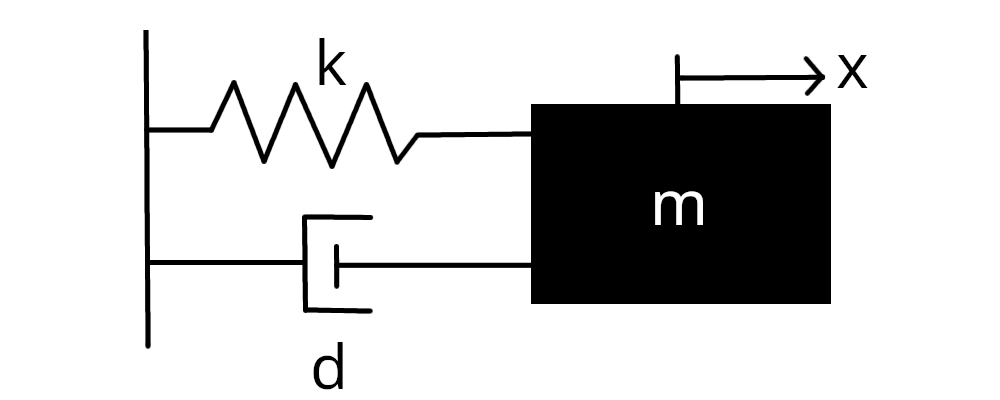
\includegraphics[height=6cm]{figs/massspringdamper.png}
    \caption{Mass spring damper system.}
    \label{fig:massspring}
\end{figure}

\noindent which can be converted into the linear two-dimensional state space ODE by defining $x_1 = x$ and $x_2 = \dot{x}$:

\begin{equation}
    \begin{bmatrix} \dot{x_1} \\ \dot{x_2} \end{bmatrix}
    = \begin{bmatrix} x_2 \\ - \frac{k}{m} x_1 - \frac{d}{m} x_2 \end{bmatrix}
    = \begin{bmatrix} 0 & 1 \\ - \frac{k}{m} & - \frac{d}{m} \end{bmatrix} \begin{bmatrix} x_1 \\ x_2 \end{bmatrix}
    \label{eq:mass_spring_damper_ode}
\end{equation}

A regression model is then trained on the mass spring damper (\ref{eq:mass_spring_damper_ode}). The parameters of the true system $k, d, m$ are all set to $1$ for simplicity. The trajectories are generated by integrating randomly sampled initial values up to $T = 10$ seconds with a sampling interval of $h = 0.1$ seconds. The initial values for generating the training data are sampled from a uniform distribution in the range $(-4, 4)$ for both variables. The target derivatives are then computed with finite differences as described above. The regression model is constructed as a feedforward neural network with four layers with the tanh activation function between each layer except the last. The model is trained with the Adam optimizer \citep{kingma2017adam} and the L2 loss function (also called MSE). The generated data is also split into a validation set to determine how well the model generalizes the data with 20 generated trajectories in each set.

Below are figures from throughout the training process displayed in the form of streamplots (sometimes called phase planes). They display a visualization of the dynamics of the system. Each line / trajectory in the streamplot will correspond to a different solution of the ODE depending on the initial value. The tangent vector of a trajectory at a point $\bm{x}$ will also correspond to the value of the derivative $\bm{f}(\bm{x})$. Streamplots can be a useful tool for visualizing the flow of a dynamical system, as long as the state space is two-dimensional.

\iffalse
\begin{figure}[H] 
    \centering
    \begin{subfigure}[t]{0.45\textwidth}
        \includegraphics[width=\textwidth]{Plots/Day2/Task2/JoystickPitch-5-5-5.eps}
    \end{subfigure}
    \begin{subfigure}[t]{0.45\textwidth}
        \includegraphics[width=\textwidth]{Plots/Day2/Task2/JoystickElevationRate-5-5-5.eps}
    \end{subfigure}
    \caption{Pitch and elevation rate response for strictly negative overlapping poles, with the joystick used as reference.}
    \label{fig:d2t2-5-5-5}
\end{figure}
\fi

\begin{figure}[H]
    \centering
    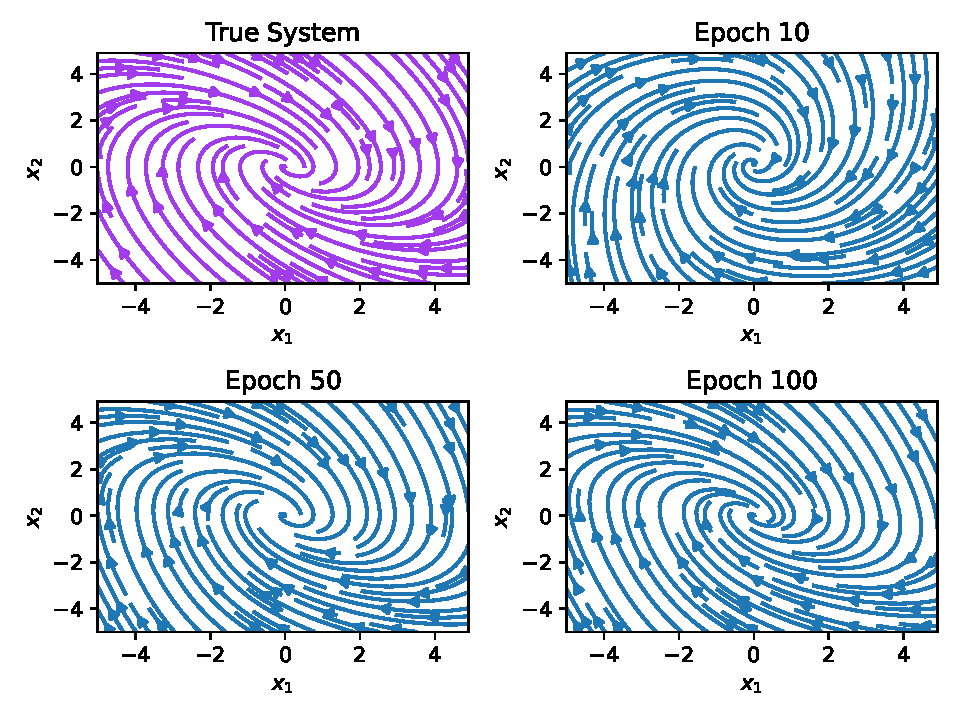
\includegraphics[height=10cm]{figs/plots/basic_experiments/mass_spring_damper_regressor_streamplot_01.pdf}
    \caption{Mass spring damper regression model streamplot.}
    \label{fig:mass_spring_damper_regressor_streamplot_01}
\end{figure}

The regression model approximates the true system well after training, as seen in Figure \ref{fig:mass_spring_damper_regressor_streamplot_01}. Because the mass spring damper system will lose energy due to the damping, all the trajectories in the streamplots converge to the origin. To measure performance in terms of loss, values for both the training and validation set are displayed below in Figure \ref{fig:mass_spring_damper_regressor_loss_01}.

\begin{figure}[H]
    \centering
    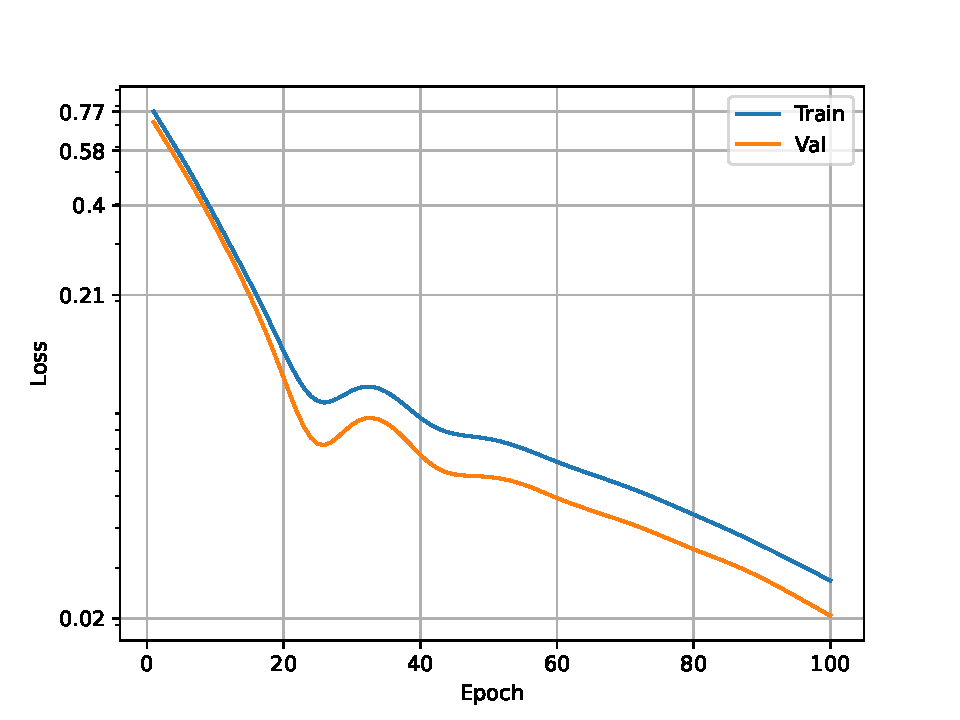
\includegraphics[height=10cm]{figs/plots/basic_experiments/mass_spring_damper_regressor_loss_01.pdf}
    \caption{Training and validation loss for the regression model learning the mass spring damper dynamics. Log scale on the y-axis.}
    \label{fig:mass_spring_damper_regressor_loss_01}
\end{figure}

Because Neural ODEs are defined as a dynamical system they can be a practical choice for learning approximations for other dynamical systems as an alternative approach to the regression model. An advantage of Neural ODEs is that they can learn dynamics without using the derivatives directly. When training a Neural ODE model, the input value is the initial value of the trajectory, and the output will be computed by integrating the initial value to a certain time. Instead of comparing a single output value it is often common to store multiple points along the trajectory when integrating to make the learning process easier.

The results from a mass spring damper learned by a Neural ODE model is shown below in Figure \ref{fig:mass_spring_damper_node_streamplot_01} and Figure \ref{fig:mass_spring_damper_node_loss_01}. The parameters are otherwise exactly the same as for the regression model.

\begin{figure}[H]
    \centering
    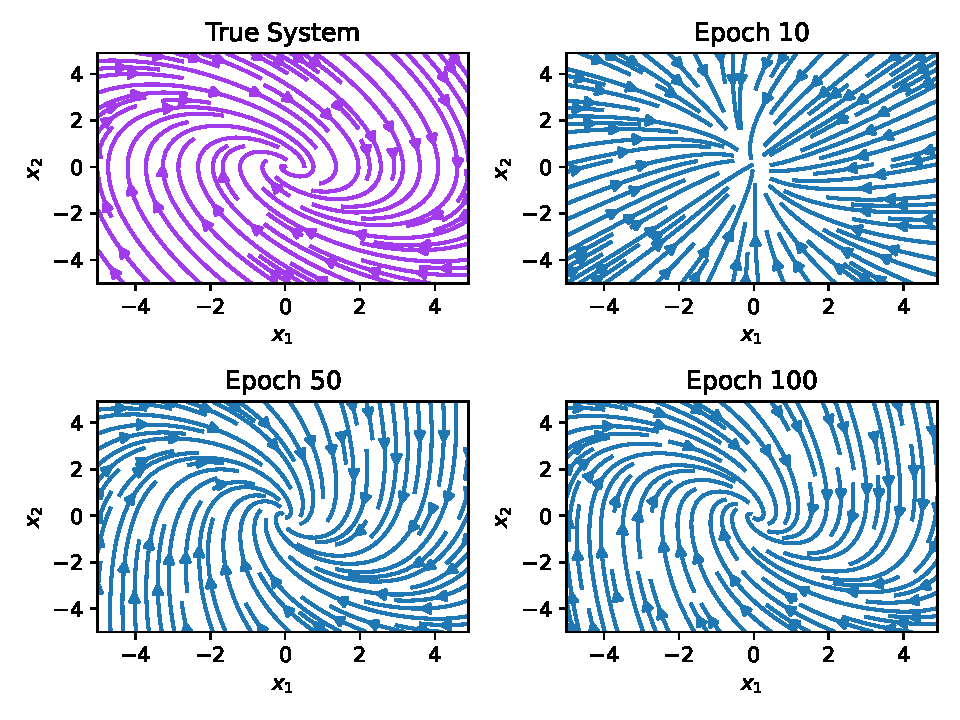
\includegraphics[height=10cm]{figs/plots/basic_experiments/mass_spring_damper_node_streamplot_01.pdf}
    \caption{Mass spring damper Neural ODE streamplot.}
    \label{fig:mass_spring_damper_node_streamplot_01}
\end{figure}

\begin{figure}[H]
    \centering
    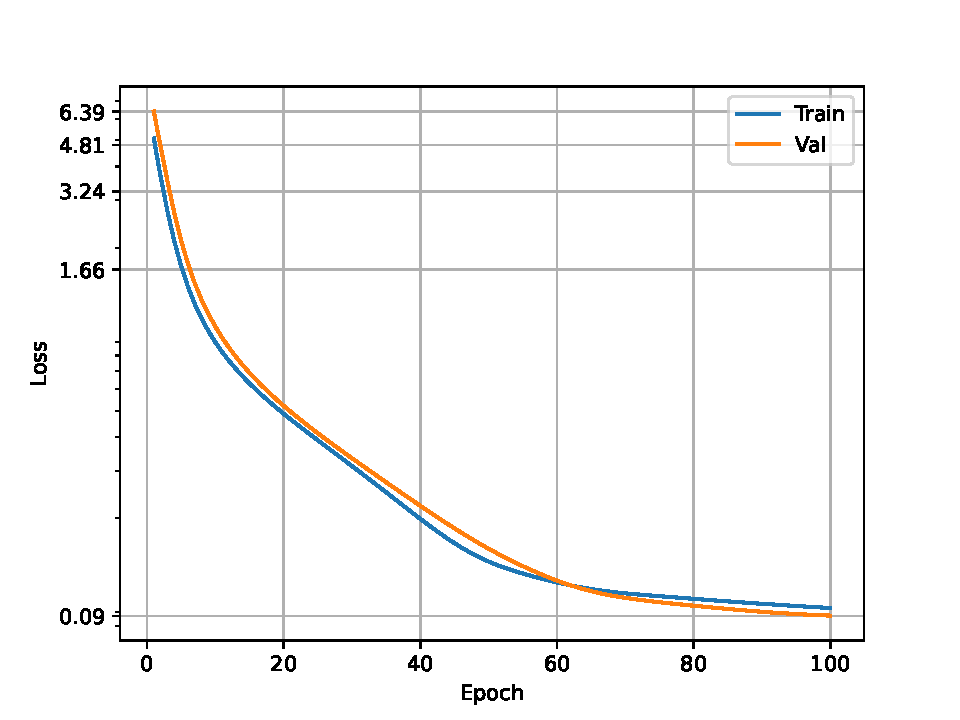
\includegraphics[height=10cm]{figs/plots/basic_experiments/mass_spring_damper_node_loss_01.pdf}
    \caption{Training and validation loss for the Neural ODE model learning the mass spring damper dynamics. Log scale on the y-axis.}
    \label{fig:mass_spring_damper_node_loss_01}
\end{figure}

The loss value of the Neural ODE is calculated by using the model to integrate initial conditions from the trajectories, and then comparing the output trajectory from the integration with the rest of the data trajectory pointwise with the L2 loss function. The values are not directly comparable to the values from the regression model.

By comparing the streamplots from Figure \ref{fig:mass_spring_damper_node_streamplot_01} with Figure \ref{fig:mass_spring_damper_regressor_streamplot_01}, the regression model approximates the true system better than the Neural ODE model at epoch 100. The performance of the regression model will to a certain extent be tied to the accuracy of the derivative target values. To see this, do the same experiment again with the change that $h = 1.0$. The resulting streamplots are shown below in Figure \ref{fig:mass_spring_damper_regressor_streamplot_1} and Figure \ref{fig:mass_spring_damper_node_streamplot_1}.

\begin{figure}[H]
    \centering
    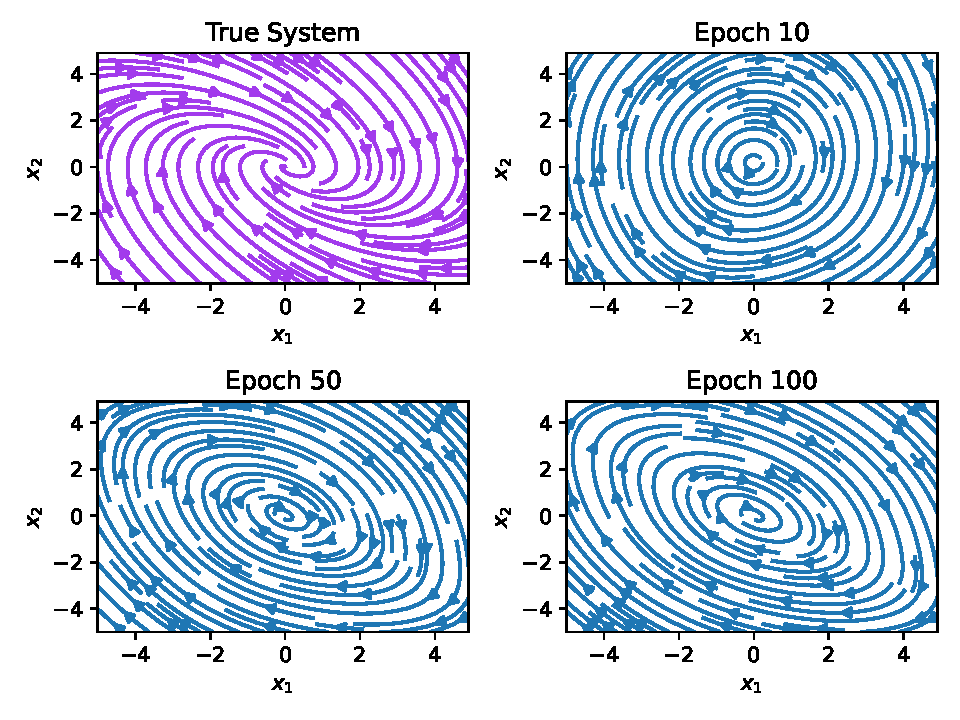
\includegraphics[height=10cm]{figs/plots/basic_experiments/mass_spring_damper_regressor_streamplot_1.pdf}
    \caption{Mass spring damper regression model streamplot with $h = 1.0$.}
    \label{fig:mass_spring_damper_regressor_streamplot_1}
\end{figure}

\begin{figure}[H]
    \centering
    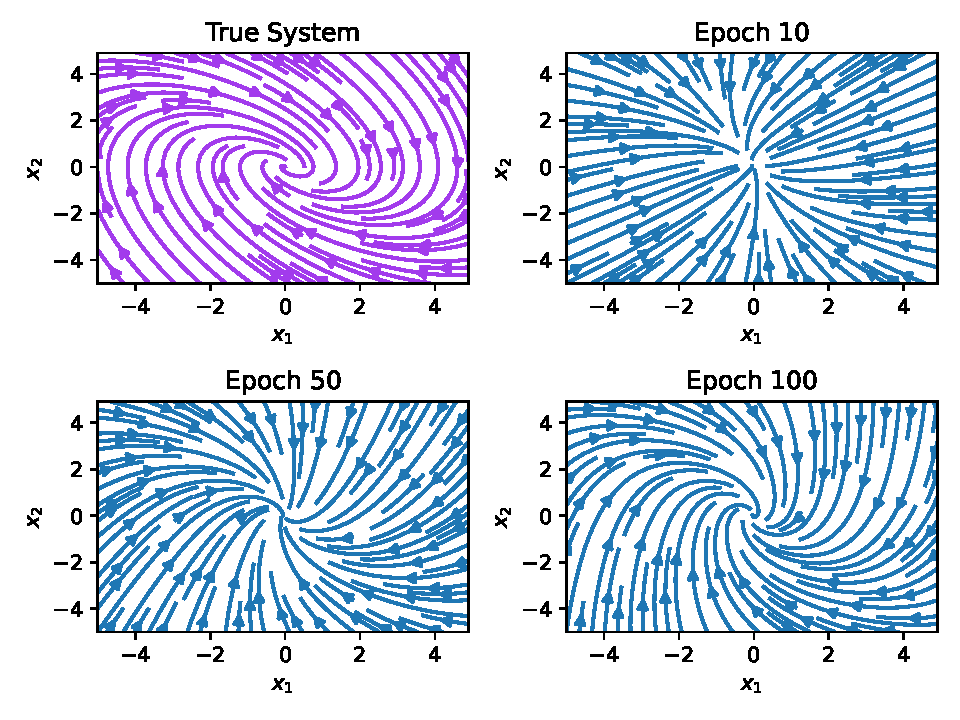
\includegraphics[height=10cm]{figs/plots/basic_experiments/mass_spring_damper_node_streamplot_1.pdf}
    \caption{Mass spring damper Neural ODE streamplot with $h = 1.0$.}
    \label{fig:mass_spring_damper_node_streamplot_1}
\end{figure}

Comparing Figure \ref{fig:mass_spring_damper_regressor_streamplot_1} to Figure \ref{fig:mass_spring_damper_regressor_streamplot_01} it looks like the regression model is not able to properly capture the dynamics that make the trajectories converge to the origin. This is a consequence of having worse approximations of the true derivatives. The Neural ODE streamplots in Figure \ref{fig:mass_spring_damper_node_streamplot_1} are similar to the streamplots in Figure \ref{fig:mass_spring_damper_node_streamplot_01} as the learning process is not as affected by the sampling interval, but it is still a little slower.

Figure \ref{fig:mass_spring_damper_trajectories} showcases some randomly selected trajectories by integrating the models trained on $h = 1.0$. The integration itself uses a value of $h=0.01$. The trajectories from the regression model converge very slowly towards the origin. The performance of the regression model is very dependent on the accuracy of the derivative targets, and numerical derivative approximations will only work with a small enough sample interval. Neural ODEs however can learn dynamics without using explicit derivatives, also with higher sample intervals. This makes them much more flexible for learning dynamical systems.

\begin{figure}[H]
    \centering
    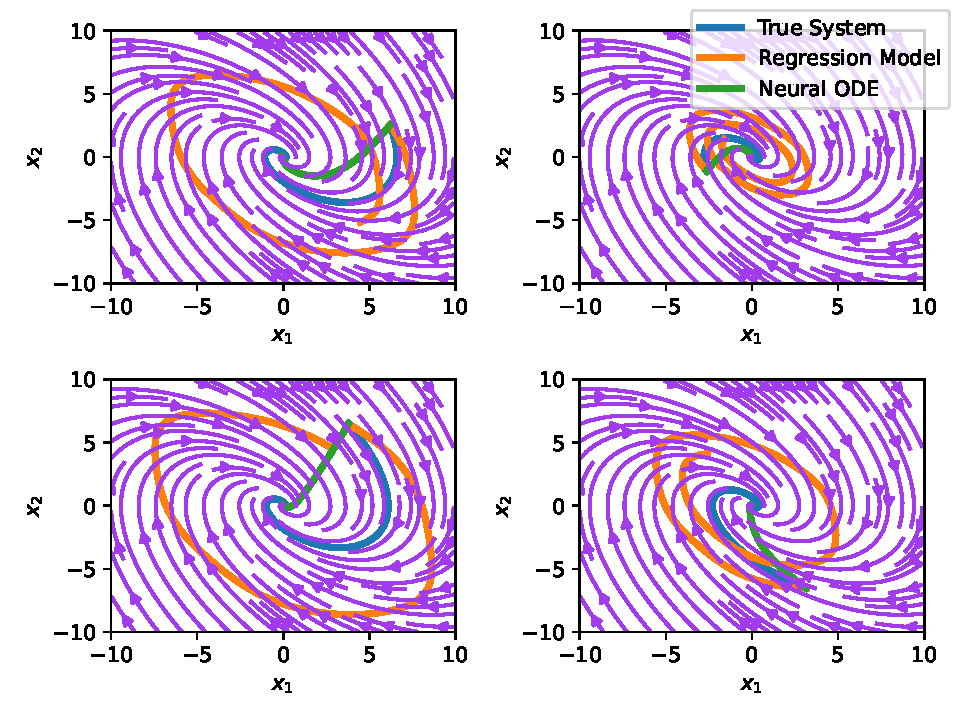
\includegraphics[height=12cm]{figs/plots/basic_experiments/mass_spring_damper_trajectories.pdf}
    \caption{Mass spring damper example trajectories.}
    \label{fig:mass_spring_damper_trajectories}
\end{figure}

Another observation from Figure \ref{fig:mass_spring_damper_trajectories} is that the trajectories from integrating the Neural ODE model tend to converge to the origin even faster than the true system. This can also be seen in Figures \ref{fig:mass_spring_damper_node_streamplot_01} and \ref{fig:mass_spring_damper_node_streamplot_1}, where both streamplots learn convergence to the origin before learning the spiraling around. A possible explanation of this phenomenon is that while the loss value is computed by comparing whole trajectories, the gradients computed by the adjoint method will be integrated from the end value to the start. This means that the initial value to the adjoint equation for the Neural ODE backwards pass always starts at the final point without considering the rest of the trajectory. As the previous experiments were done with a final time of $T = 10$ seconds, most of the trajectories used in the training process would converge to the origin. This is also demonstrated in Figure \ref{fig:mass_spring_damper_trajectories} where all the randomly chosen examples converge to the origin.

More trajectories that converge to different points are needed to enhance the learning process for Neural ODE. Reduce the end time $T$ from $10$ to $1$ second, and set $h = 0.1$. The training losses are unchanged, but the validation loss for the regression model is now changed to make it directly comparable with the Neural ODE model. This means that the loss value is calculated by using the regression model as a dynamics function and then integrating initial values to generate trajectories. These trajectories are then compared with the target trajectories with the L2 loss. The resulting losses from these experiments displayed in Figure \ref{fig:mass_spring_damper_loss_comparison_h01_T1} shows that the Neural ODE model now slightly outperforms the regression model when the end time of the trajectories are shortened to avoid origin convergence.

\begin{figure}[H]
    \centering
    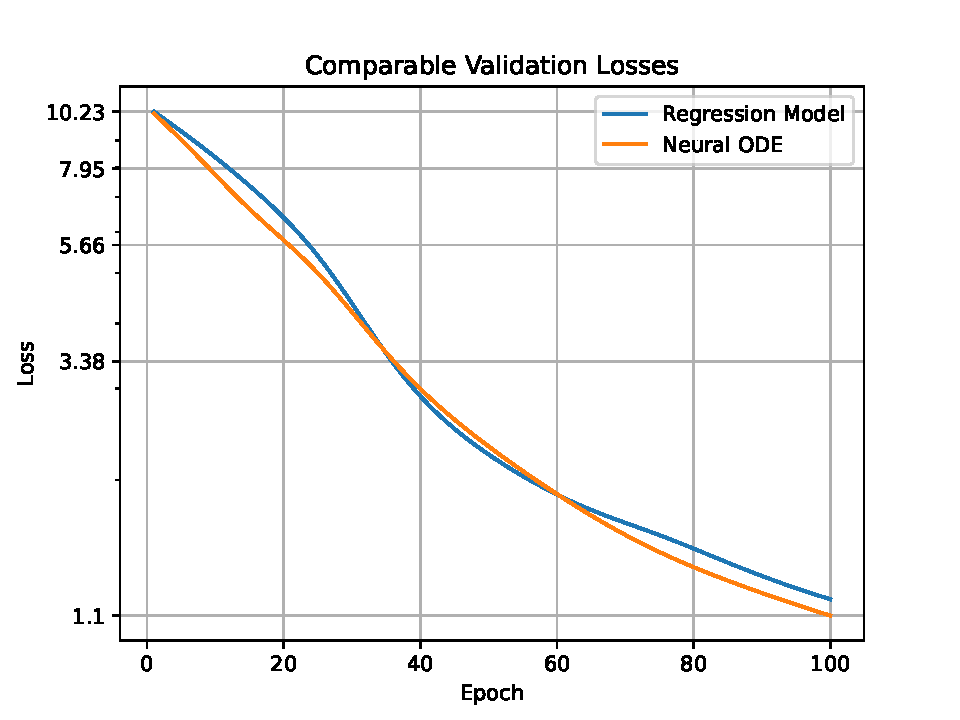
\includegraphics[height=10cm]{figs/plots/basic_experiments/mass_spring_damper_loss_comparison_h01_T1.pdf}
    \caption{Validation losses for both the regression model and the Neural ODE model when learning the mass spring damper dynamics. $T = 1$ and $h = 0.1$. Log scale on the y-axis.}
    \label{fig:mass_spring_damper_loss_comparison_h01_T1}
\end{figure}

The parameters were then changed back to an ending time of $T = 10$ seconds with $h = 1.0$. The trajectory generation was also changed so that they end further away from the origin. The results are displayed in Figure \ref{fig:mass_spring_damper_loss_comparison_h1_T10}. Neural ODEs clearly outperforms regression models when the accuracy of the derivative approximations decrease and when the trajectories are more varied in behavior.

\begin{figure}[H]
    \centering
    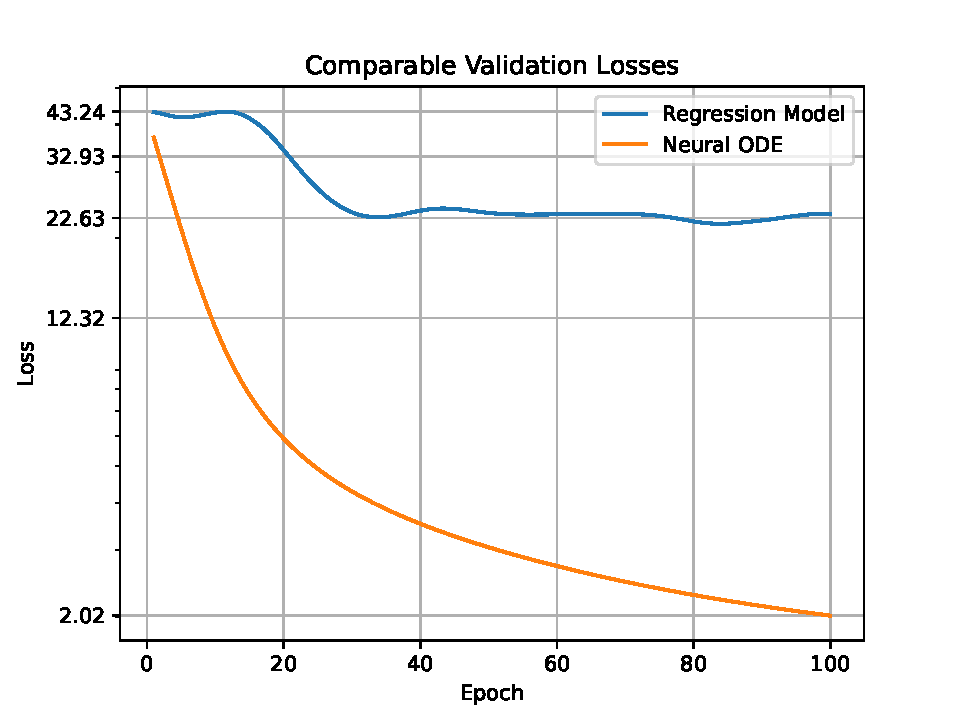
\includegraphics[height=10cm]{figs/plots/basic_experiments/mass_spring_damper_loss_comparison_h1_T10.pdf}
    \caption{Validation losses for both the regression model and the Neural ODE model when learning the mass spring damper dynamics. $T = 10$ and $h = 1.0$.}
    \label{fig:mass_spring_damper_loss_comparison_h1_T10}
\end{figure}

Because the mass spring damper is a stable linear system it is not surprising that the models are able to learn the dynamics this well. To see an example of a nonlinear system, consider the dynamics of a pendulum given by the ODE:

\begin{equation}
    \ddot{\theta} = - \frac{g}{l} \sin{\theta}
    \label{eq:single_pendulum_ode_secondorder}
\end{equation}

\begin{figure}[H]
    \centering
    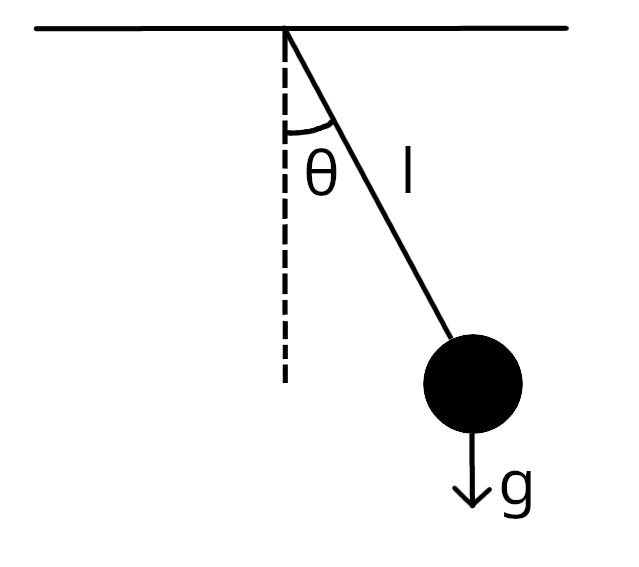
\includegraphics[height=6cm]{figs/singlependulum.png}
    \caption{Pendulum system.}
    \label{fig:singlependulum}
\end{figure}

\noindent which can be converted into the state space ODE by defining $x_1 = \theta$ and $x_2 = \dot{\theta}$ in the same way as the mass spring damper ODE:

\begin{equation}
    \begin{bmatrix} \dot{x_1} \\ \dot{x_2} \end{bmatrix}
    = \begin{bmatrix} x_2 \\ - \frac{g}{l} \sin{x_1} \end{bmatrix}
    \label{eq:single_pendulum_ode}
\end{equation}

Both a regression model and a Neural ODE are trained on trajectories from the pendulum with the same basic setup as the mass spring damper. Two additional layers are added to the neural networks and the amount of training data has been increased from 20 trajectories to 200 because of the added complexity of the pendulum dynamics. $T = 1$ second and $h = 0.1$. The model is also trained for 1000 epochs now up from 100. The initial values for generating the training data are sampled from a uniform distribution in the range $(-10, 10)$ for both variables.

The evolution of the streamplots for both models are displayed below in Figure \ref{fig:single_pendulum_regressor_streamplot} and Figure \ref{fig:single_pendulum_node_streamplot}

\begin{figure}[H]
    \centering
    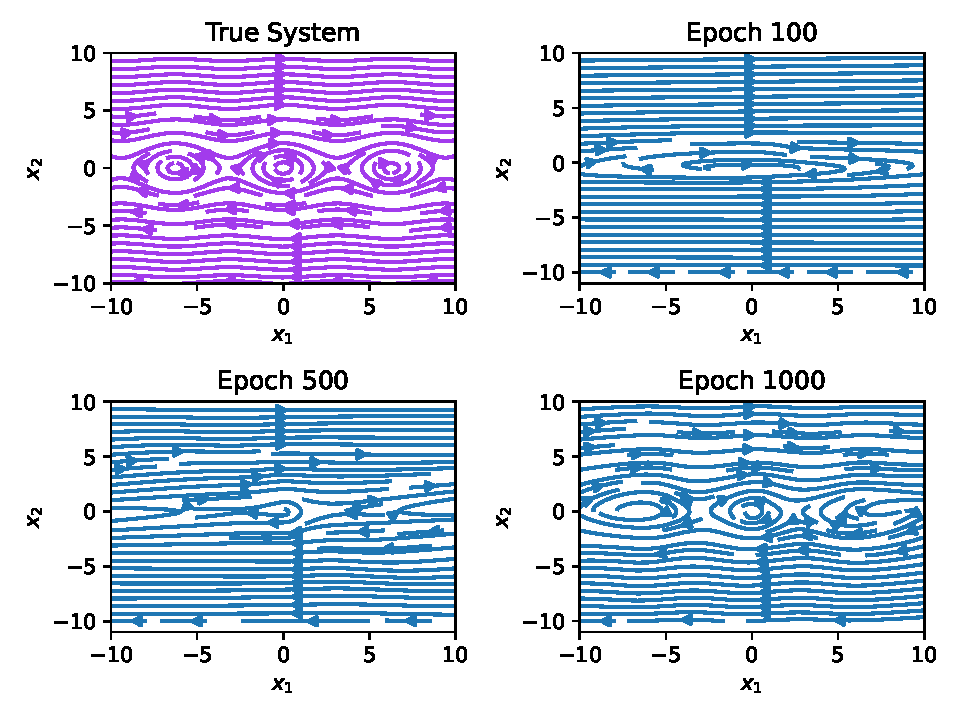
\includegraphics[height=10cm]{figs/plots/basic_experiments/single_pendulum_regressor_streamplot.pdf}
    \caption{Pendulum system regression model streamplot.}
    \label{fig:single_pendulum_regressor_streamplot}
\end{figure}

\begin{figure}[H]
    \centering
    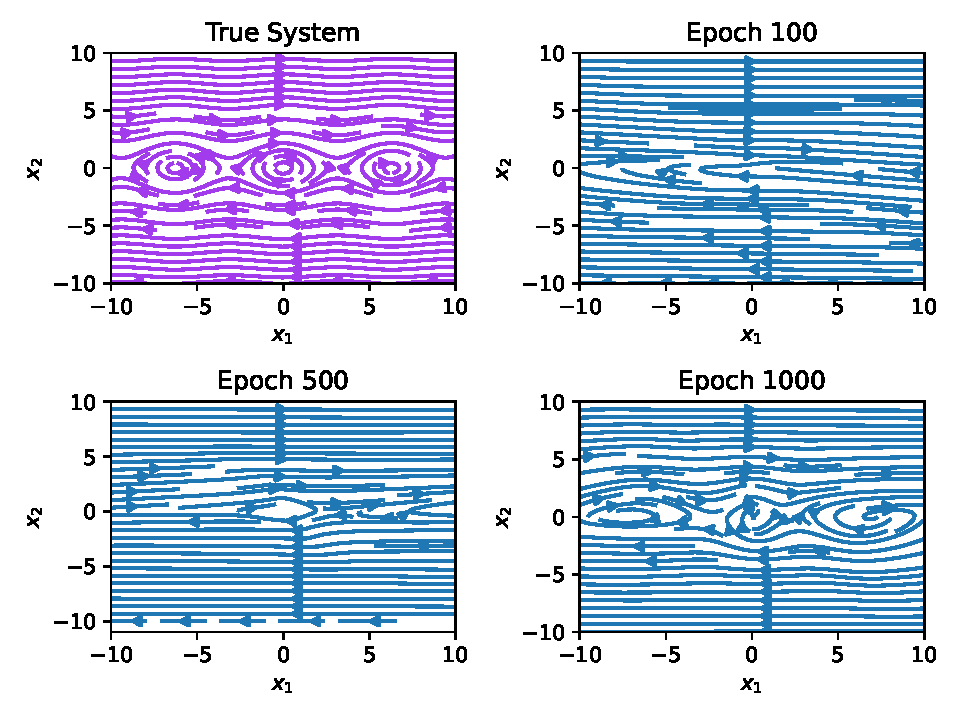
\includegraphics[height=10cm]{figs/plots/basic_experiments/single_pendulum_node_streamplot.pdf}
    \caption{Pendulum system regression Neural ODE streamplot.}
    \label{fig:single_pendulum_node_streamplot}
\end{figure}

The dynamics of the pendulum is significantly more difficult to learn compared to the mass spring damper, requiring many more epochs of training. Both models are able to quickly learn the rotation around the origin. This can be explained because the pendulum dynamics are approximately linear around its origin, meaning $\sin{\theta} \approx \theta$ for small values of $\theta$. Both models also start to capture the dynamics of the other equilibrium points at epoch 1000. More data sampled from a larger area might be needed to generalize even further.

The validation losses of both models are displayed together in Figure \ref{fig:single_pendulum_loss_comparison_h01_T1}. The validation losses are again computed by using the trained models to integrate initial values, and then comparing trajectories pointwise with the L2 loss function. The integration for calculating the validation losses is done with $h = 0.01$.

\begin{figure}[H]
    \centering
    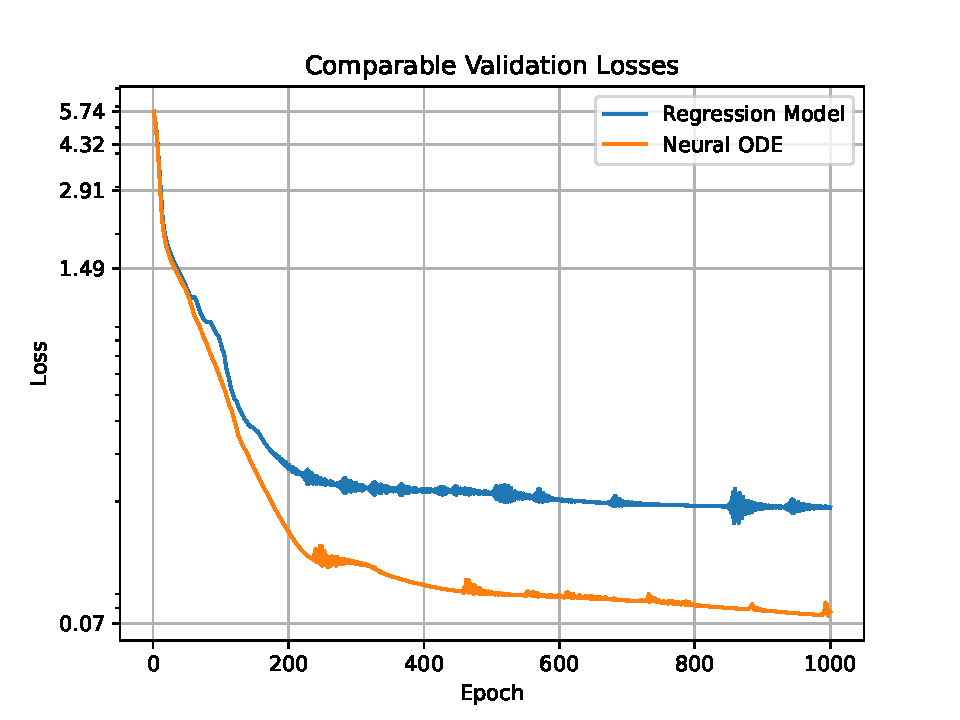
\includegraphics[height=10cm]{figs/plots/basic_experiments/single_pendulum_loss_comparison_h01_T1.pdf}
    \caption{Validation losses for both the regression model and the Neural ODE model when learning the pendulum dynamics. Log scale on the y-axis.}
    \label{fig:single_pendulum_loss_comparison_h01_T1}
\end{figure}

The Neural ODE learns the dynamics slightly faster at the beginning but eventually stops learning. The regression model at the start, but eventually stops learning, while the regression model keeps getting better. in terms of accurately integrating trajectories, with the given training parameters.

Overall, learning simple dynamical systems with deep learning based models are possible. Similarly to most problems in deep learning, the quality of the model will be dependent on the training data. If the derivatives are explicitly given, or can be approximated based on the available data, training a regression model is the most straightforward approach. Neural ODEs will often be on par with regression models in terms of performance, but suffer from a slower training process. If the derivatives are unavailable or the sampling interval is too high to approximate them, then Neural ODEs will outperform a simple regression model.

\section{Learning Non-Homeomorphic Flows}

There are some types of systems that the regression model is unable to represent. One example first demonstrated by \citep{dupont2019augmented} is regarding non-homeomorphic flows. A flow in this context basically means the solution trajectory of an ODE. For a function to be homeomorphic it must be a bijection, continuous and the inverse function must also be continuous. An equivalent formulation is that the function is preserving the topological structure of the input and output spaces. To see an example of a non-homeomorphic flow, consider the scalar ODE $\dot{x} = f(x)$ and two flows / solutions $x_1(t)$ and $x_2(t)$ with the following properties:

\begin{equation}
    \begin{aligned}
    x_1(0) = 1 & \qquad & x_2(0) = -1 \\
    x_1(1) = -1 & \qquad & x_2(1) = 1
    \end{aligned}
    \label{eq:straightlines}
\end{equation}

An example of flows with these properties can be visualized in Figure \ref{fig:nonhomeomorphicflows} with $x_1(t)$ in blue and $x_2(t)$ in red. The reason for why a regression model is unable to represent these flows is because it is impossible to define an ODE $\dot{x} = f(x)$ which gives these flows as solutions \citep{dupont2019augmented}. Intuitively, it is not possible for ODE solution trajectories to intercept each other because that would mean that the derivatives $f(x(t))$ at the intersection point must have at least two different values, which of course is impossible.

\begin{figure}[H]
    \centering
    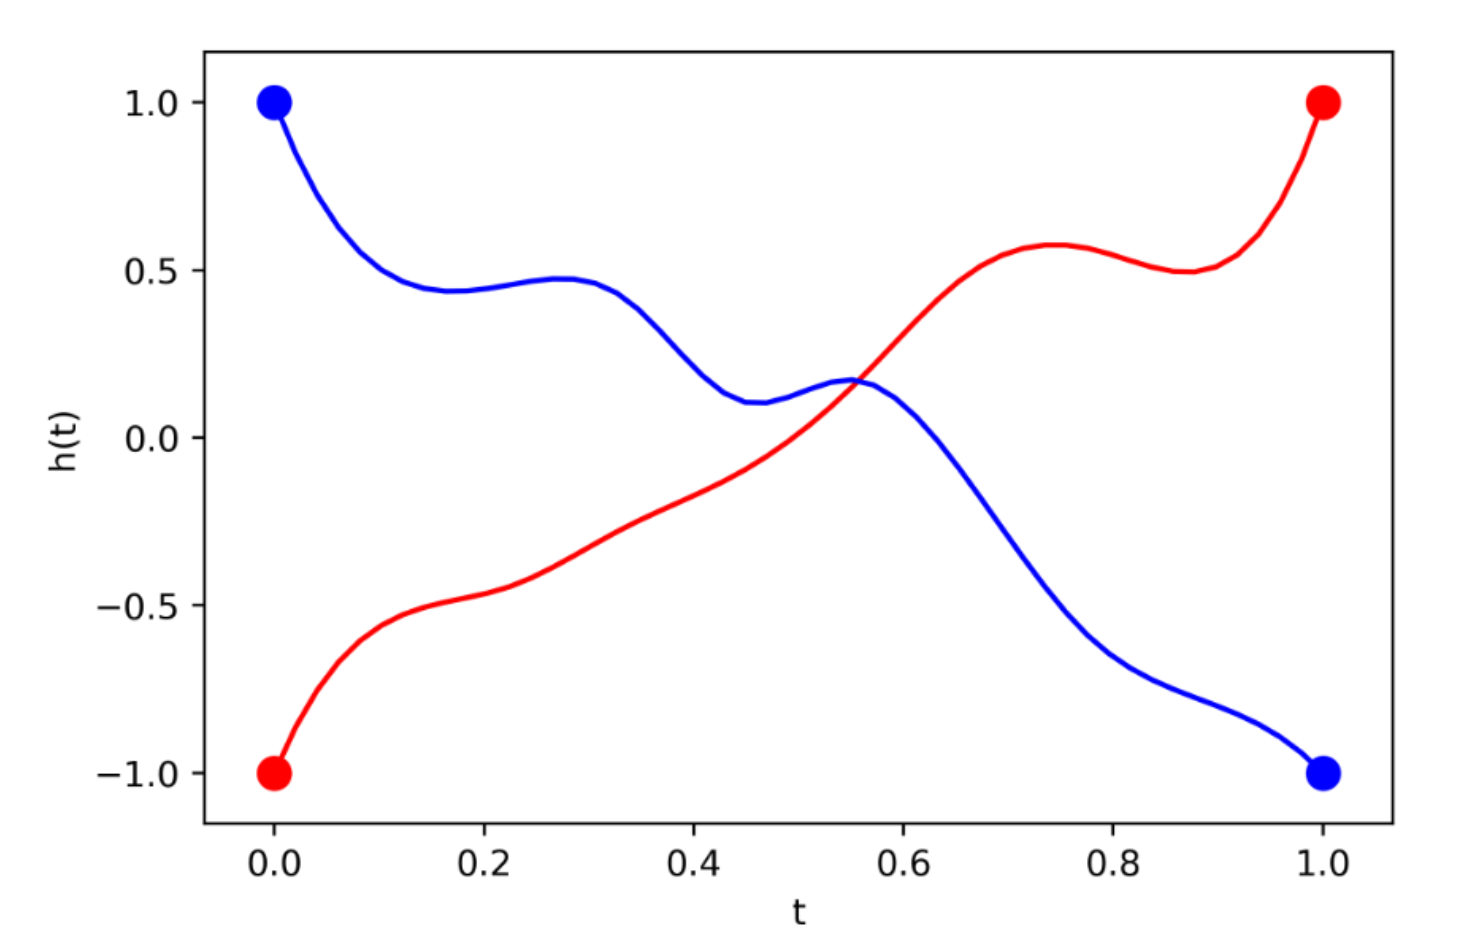
\includegraphics[height=8cm]{figs/nonhomeomorphicflows.png}
    \caption{Example of a non-homeomorphic flow. Figure taken from \cite{dupont2019augmented}.}
    \label{fig:nonhomeomorphicflows}
\end{figure}

It is also impossible to train a standard Neural ODE model to learn these flows. Trying anyway can be done by creating two trajectories equal to straight lines matching the properties of (\ref{eq:straightlines}) and then training a Neural ODE on these two trajectories. The resulting streamplot is shown in Figure \ref{fig:nonhomeomorphicflows_node}. The streamplot shows that the solutions are unable to cross each other, resulting in all trajectories converging to 0.

\begin{figure}[H]
    \centering
    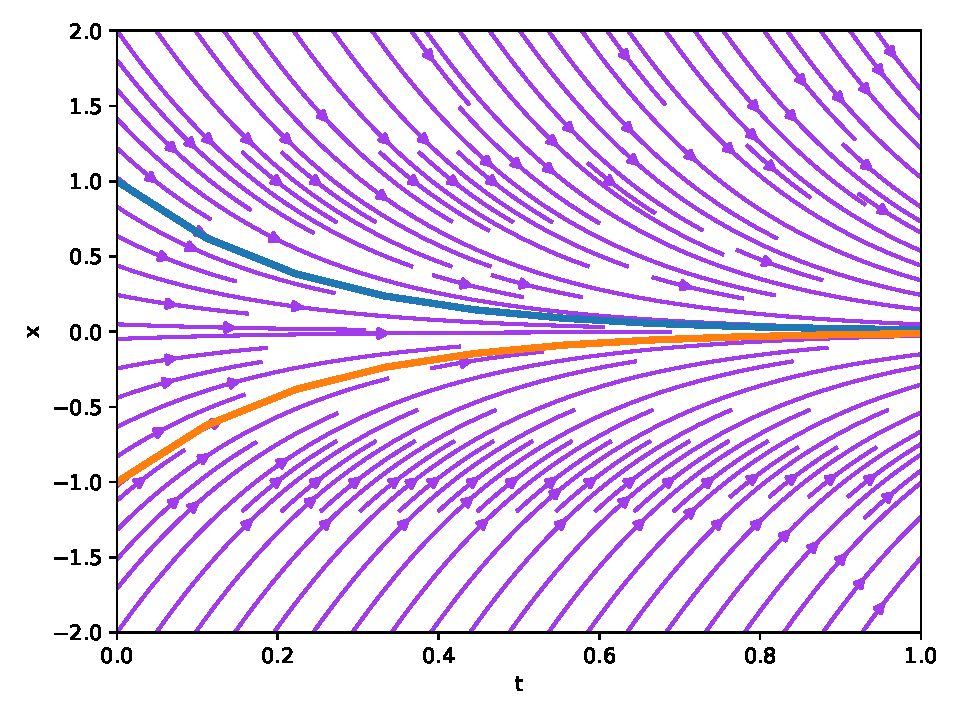
\includegraphics[height=10cm]{figs/nonhomeomorphicflows_node.pdf}
    \caption{Streamplot after training a standard Neural ODE on a non-homeomorphic flow.}
    \label{fig:nonhomeomorphicflows_node}
\end{figure}

What \cite{dupont2019augmented} showed is that Neural ODEs can be augmented to overcome this problem. Augmenting in this case means to add additional dimensions to the state $\bm{x}$ with initial values of 0. Solution trajectories can then essentially use the extra dimensions to move around the intersection point. Using the same problem formulation as above but adding one extra augmented dimension to the Neural ODE makes it possible to create the described flow. A plot of this is shown in Figure \ref{fig:nonhomeomorphicflows_anode}, where the trajectories are projected down onto the first original dimension.

\begin{figure}[H]
    \centering
    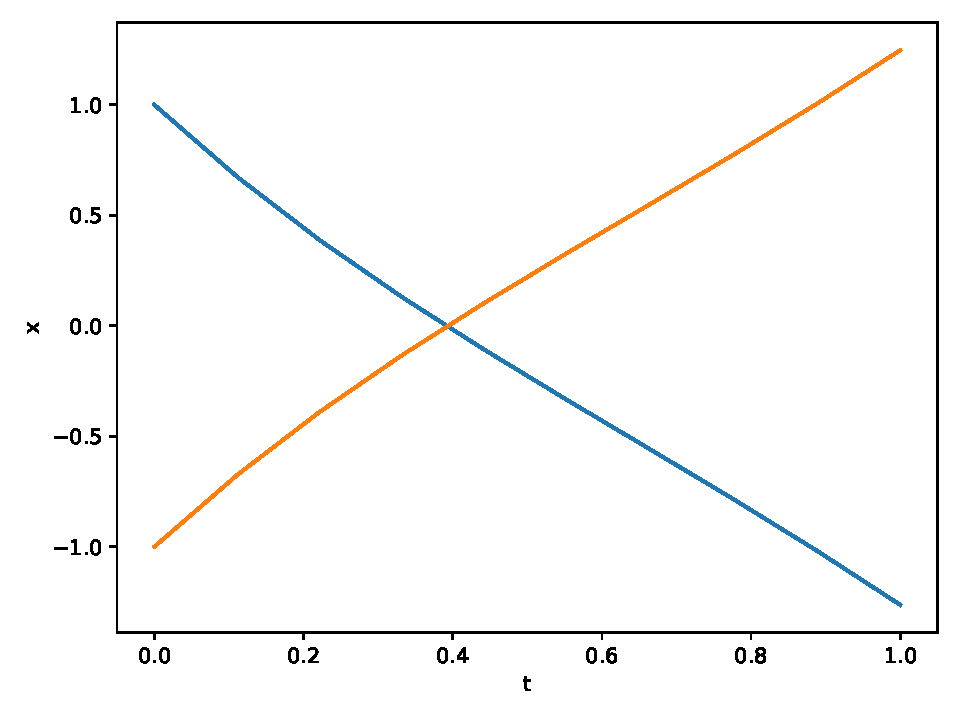
\includegraphics[height=10cm]{figs/nonhomeomorphicflows_anode.pdf}
    \caption{Training an augmented Neural ODE on a non-homeomorphic flow.}
    \label{fig:nonhomeomorphicflows_anode}
\end{figure}

\cite{dupont2019augmented} also showed that adding extra augmented dimensions can often increase the performance and training speed of Neural ODEs for representation learning. The number of augmented dimensions can in these cases be considered a hyperparameter and part of the model structure. Although when the goal is to learn a dynamical system directly, augmented models are less useful as the new augmented states do not map directly back to the original states.

\section{Learning Non-Autonomous Dynamical Systems}

An autonomous dynamical system is any system that can be described by the ODE: $\dot{\bm{x}} = \bm{f}(\bm{x})$. A non-autonomous system has dynamics that explicitly depends on the independent variable $t$ so that the ODE becomes: $\dot{\bm{x}} = \bm{f}(t, \bm{x})$. Non-autonomous systems have the expressive capabilities to model many more types of dynamical systems than the standard autonomous systems. They are particularly useful for modeling systems that are driven by some external input (hence the name). For example could it be possible to derive an ODE that describes the motion of the human body, but since the motion of the body is controlled by signals from the brain it is possible to consider these input signals as time-varying and incorporate them into a non-autonomous model.

Standard Neural ODEs are represented with ANNs that take a state $\bm{x}(t)$ as input. To learn a non-autonomous system it is also necessary to somehow use the independent variable $t$. Consider the 1-dimensional Riccati equation:

\begin{equation}
    \dot{x} = x^2 - t
    \label{eq:riccati}
\end{equation}

\noindent with streamplot shown in Figure \ref{fig:riccati_true}. There are two time-varying equilibrium points for the system at $x(t) = \pm \sqrt{t}$.

\begin{figure}[H]
    \centering
    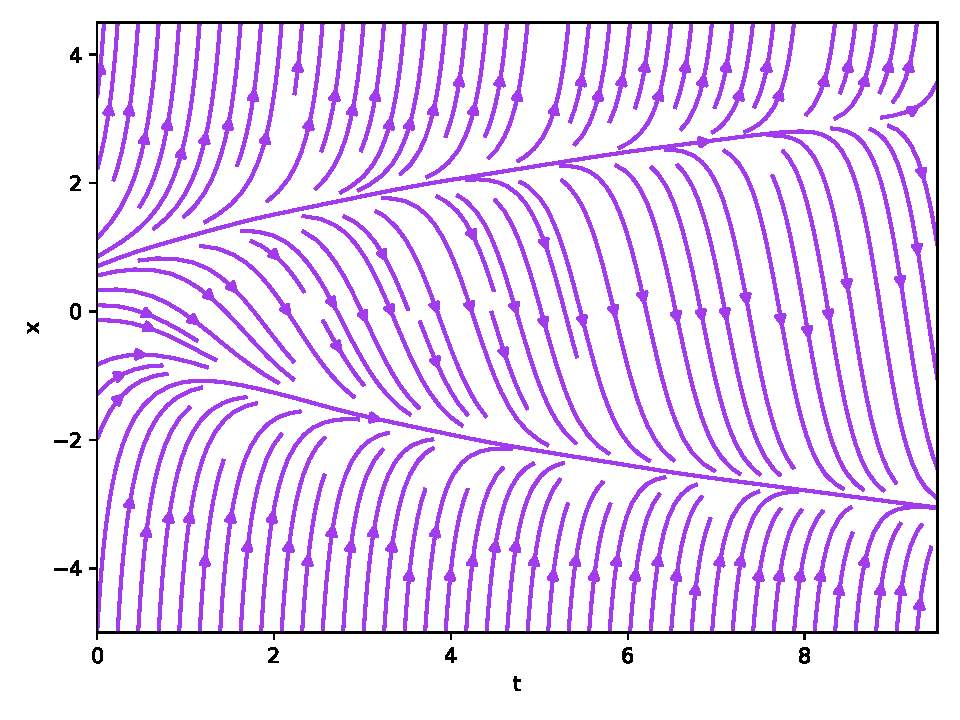
\includegraphics[height=10cm]{figs/riccati_true.pdf}
    \caption{Riccati equation streamplot.}
    \label{fig:riccati_true}
\end{figure}

Training a standard autonomous Neural ODE on trajectories from the Riccati equation results in the streamplot shown in Figure \ref{fig:riccati_node}. It is not able to learn the time-varying equilibrium points and makes every trajectory move very little in regards to time.

\begin{figure}[H]
    \centering
    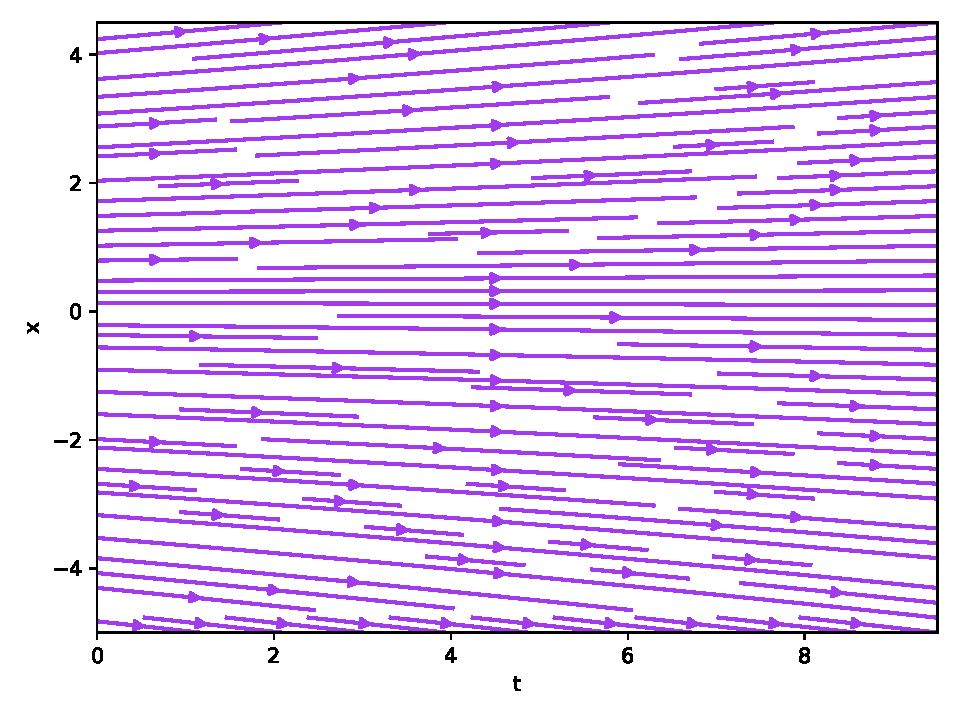
\includegraphics[height=10cm]{figs/riccati_node.pdf}
    \caption{Neural ODE trained on the Riccati equation streamplot.}
    \label{fig:riccati_node}
\end{figure}

Adding an explicit time-dependence to the Neural ODE can be done in many different ways. The simplest is to simply augment the neural network with time as an additional input. This could work for the Riccati equation as there is only one state otherwise, but for a system with many more states, adding one extra with time might not be able to properly capture the importance of the time. A slightly more sophisticated approach is to create one network that takes in the time and increases the dimension. Another network can then take the state as input and increase the state to the same dimension as time. The two output vectors can then be concatenated and sent into a third network which produces the final output. Training a Neural ODE based on this architecture results in the streamplot shown in Figure \ref{fig:riccati_nodetime}. 

\begin{figure}[H]
    \centering
    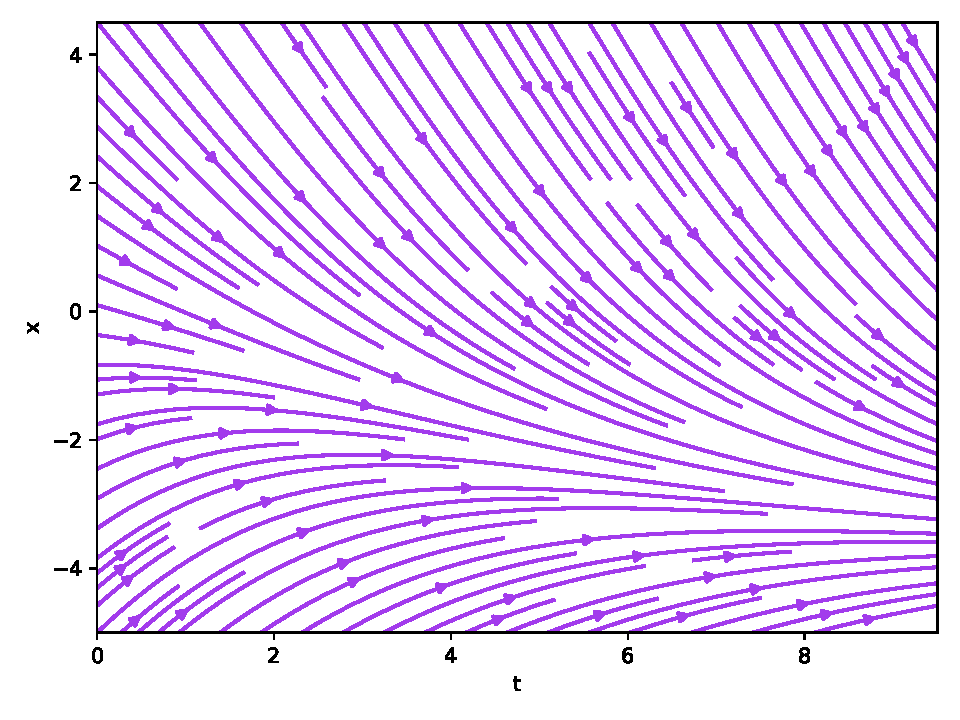
\includegraphics[height=10cm]{figs/riccati_nodetime.pdf}
    \caption{Neural ODE with explicit time-dependence trained on the Riccati equation streamplot.}
    \label{fig:riccati_nodetime}
\end{figure}

Can now see that the time-dependent Neural ODE was capable of learning the time-varying equilibrium point at $x(t) = - \sqrt{t}$. The other equilibrium point at $x(t) = \sqrt{t}$ proved more difficult to learn because of a lack of training trajectories. Since it is unstable it is not easy to generate trajectories above the equilibrium point as they quickly converge to infinity. From (\ref{eq:riccati}) can see that when $x^2 >> 0$ the dynamics becomes: $\dot{x} \approx x^2$. Solutions to this approximated ODE take the form: $x(t) = \frac{1}{c - t}$ for some constant $c$. These solutions have the property that they diverge to infinity in finite time, more specifically at $t = c$ which makes it difficult to generate training trajectories.

\cite{timedependencenode} explored other approaches to adding time-dependencies to Neural ODEs. They experimented with making the parameters of the neural network represented as various functions of time. One of these approaches included having separate neural networks that takes the time as input and outputs the parameters for the other neural network.

Because many real life systems are inherently non-autonomous it can be useful to add time-dependencies to properly learn the dynamics of these systems. As shown by \cite{timedependencenode}, adding a time-dependency can also increase the general expressive capabilities of Neural ODEs and can also make them able to learn non-homeomorphic flows.

\chapter{Motion Classification}
\label{cha:motionclassification}

This chapter uses concepts from vector calculus, and explores a novel idea for classifying trajectories sampled from dynamical systems by training Neural ODEs.

\section{Introduction}
\label{sec:motionclassificationintroduction}

Time-series classification is a type of classification problem where the input data are time-series / sequences of datapoints where the order of the datapoints in the sequence has importance. The output classes are dependent on the specific problem. For example could the whole sequence of datapoints be of a certain class. Another possibility is that each datapoint in the sequence corresponds to a class. This thesis uses the first of these options where whole sequences are classified. Time-series classification can be framed as a supervised learning problem where a classifier model is trained on the available training dataset. As mentioned in section \ref{sec:deeplearning}, Recurrent Neural Networks (RNNs) can often work well on learning sequential data making them useful for constructing a classification model.

Motion classification can be thought of as a time-series classification problem where the inputs are trajectories generated by mechanical systems. The outputs can for example be what type of mechanical system generated the trajectories. A practical use case can be to classify and detect movement-related problems for humans in a medical setting.

Because mechanical systems produce motions in continuous time, the trajectory generating processes can then be thought of as two or more dynamical systems. Assume for now that it is a binary classification problem, so that there are two different generating systems, here represented as ODEs:

\begin{equation*}
    \begin{aligned}[c]
        \dot{\bm{x}} = \bm{f}(t, \bm{x})
    \end{aligned}
    \qquad \qquad
    \begin{aligned}[c]
        \dot{\bm{x}} = \bm{g}(t, \bm{x})
    \end{aligned}
\end{equation*}


It could also be possible to perform time-series classification on other types of dynamical systems such as PDEs or SDEs, but this is not investigated in this master thesis.

\iffalse
Another assumption for the problem to make sense is that the samples from both systems have relatively similar values. This means that if the initial conditions are samples from some random distribution, the two dynamical systems should have the same random distribution of initial conditions so that the different classes of trajectories start at similar values. The two dynamical systems should also be similar to each other in the sense that trajectories should converge to the same equilibrium points. For example, if one of the dynamical systems is unstable so that every trajectory diverges to infinity, while the other always converges to the origin, the classification can also be done trivially.
\fi

The problem can now be stated as a binary classification problem: given samples $\bm{x}_1, \bm{x}_2, \dots, \bm{x}_N$ from a continuous time trajectory $\bm{x}(t)$, determine if the samples were generated by $\bm{f}$ or $\bm{g}$. It is assumed that both systems have the same dimension, otherwise the classification problem is trivial. A simple baseline model is constructed with an RNN by first sending inputs into a Long Short Term Memory (LSTM). The final hidden states from the LSTM can then be used as inputs to a classifier head which can be constructed as a feedforward neural network. RNNs are a class of neural networks where there are additional connections going through the elements in the input sequence. An LSTM is a specific architecture which implements these connections in a particular method.

RNN-based models like these are simple to construct, but lack any type of domain knowledge about the problem. Motion classification is based on continuous dynamical systems, which motivates the use of Neural ODEs for classification purposes. A classification method based on Neural ODEs is derived in the next section.

\section{The Line Integral Loss Function}
\label{sec:lineintegralloss}

A line integral from vector calculus is an integral where the function $\bm{f}$ to be integrated is evaluated over a 1-dimensional curve $\Gamma$. The function can either be a scalar field mapping $f: \mathbb{R}^n \rightarrow \mathbb{R}$ where $f$ is evaluated and integrated over $\Gamma$, or a vector field mapping $\bm{f}: \mathbb{R}^n \rightarrow \mathbb{R}^n$ where the components of $\bm{f}$ that aligns with $\Gamma$ are evaluated and integrated over $\Gamma$. For the vector field case, define the line integral as:

\begin{equation}
    \int_{\Gamma} \bm{f} \cdot d \bm{r} = \int_{t_0}^{t_1} \bm{f}(\bm{r}(t)) \cdot \bm{r}'(t) dt
\end{equation}

\noindent where $\bm{r}(t): [t_0, t_1] \rightarrow \mathbb{R}^n$ is a parametrization of $\Gamma$. All curves have an infinite number of different parametrizations. An example that shows this is the following: define $\Gamma$ as a straight line in $\mathbb{R}^2$ going from the point $(0, 0)$ to the point $(2, 1)$. A simple parametrization is $\bm{r}_1(t) = \begin{bmatrix} 2 t & t \end{bmatrix}^T$ with $0 \leq t \leq 1$. Another parametrization of the same curve is given as $\bm{r}_2(t) = \begin{bmatrix} 8 t^2 & 4 t^2 \end{bmatrix}^T$ with $0 \leq t \leq 0.5$. More generally, curves are uniquely defined up to every possible homeomorphism of $t$.

Because $\bm{r}'(t) = \frac{d \bm{r}(t)}{dt}$ will evaluate to vectors that are tangential to the curve, the dot product between $\bm{f}$ and $\bm{r}'(t)$ will be the largest when $\bm{f}$ and $\bm{r}$ are pointing in the same direction and the smallest when they are pointing in the opposite direction.

\begin{figure}[H]
    \centering
    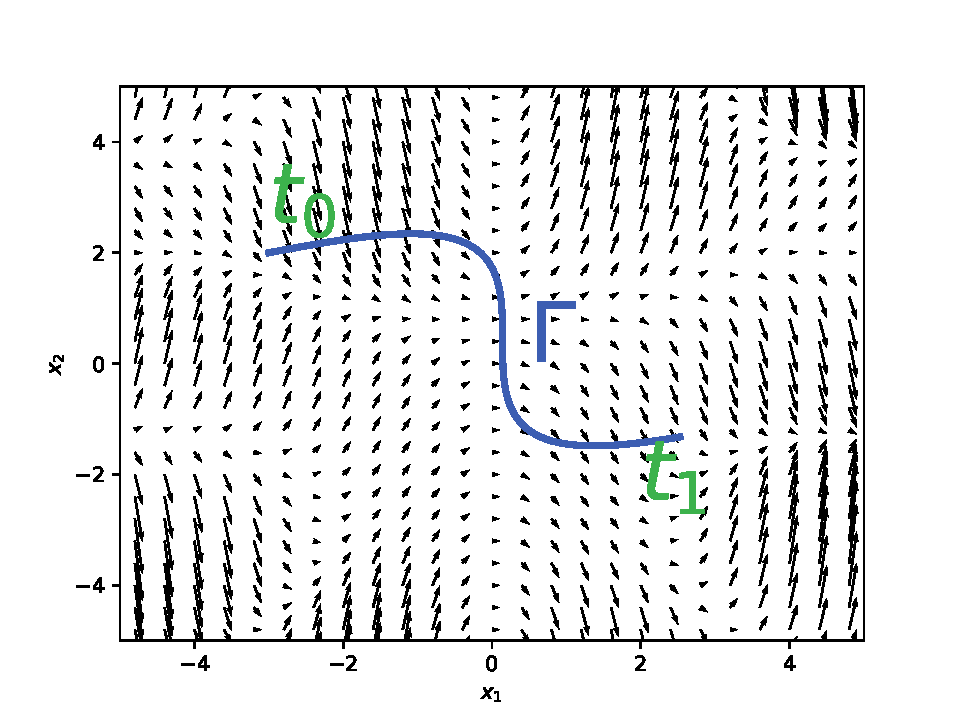
\includegraphics[height=12cm]{figs/plots/motion_classification/line_integral.pdf}
    \caption{Example of a curve $\Gamma$ and a vector field $\bm{f}$.}
    \label{fig:line_integral_field}
\end{figure}

When training Neural ODEs, the training data are trajectories which form curves in the vector space, while the Neural ODE learns a vector field that fits these trajectories. This means that if a line integral is computed over these trajectories, its value will increase during the training process of the Neural ODE. A novel idea from this master thesis is to use this line integral directly as a new loss function for training Neural ODEs. This setup can be formulated as solving the optimization problem:

\begin{equation}
    \begin{aligned}
        \max_{\bm{\theta}} \quad & \frac{1}{n} \sum_{k=1}^{n} \int_{t_{k_0}}^{t_{k_1}} \bm{f}(t, \bm{r}_k(t); \bm{\theta}) \cdot \bm{r}_k'(t) dt
    \end{aligned}
    \label{eq:lineintegralmax}
\end{equation}

\noindent where $\bm{f}(t, \bm{r}_k(t); \bm{\theta})$ is a vector field parametrized by $\bm{\theta}$ and the line integrals for each trajectory $\bm{r}_k(t)$ are averaged over the training set indexed by $k = 1 \dots n$. Define the loss function as:

\begin{equation}
    \begin{aligned}
        \mathcal{L} = - \frac{1}{n} \sum_{k=1}^{n} \int_{t_{k_0}}^{t_{k_1}} \bm{f}(t, \bm{r}_k(t); \bm{\theta})^T \bm{r}_k'(t) dt
    \end{aligned}
\end{equation}

\noindent with a minus in front of the average because of the convention in deep learning to minimize the loss function.

To train a model with this loss function it is necessary to compute gradients to the parameters $\frac{\partial \mathcal{L}}{\partial \bm{\theta}}$ so that the optimization problem can be solved. The gradients can be found by:

\begin{equation}
    \begin{aligned}
        \frac{\partial \mathcal{L}}{\partial \bm{\theta}}
        &= - \frac{\partial}{\partial \bm{\theta}} \begin{bmatrix} \frac{1}{n} \sum_{k=1}^{n} \int_{t_{k_0}}^{t_{k_1}} \bm{f}^T \bm{r}_k' dt \end{bmatrix} \\
        &= - \frac{1}{n} \sum_{k=1}^{n} \frac{\partial}{\partial \bm{\theta}} \begin{bmatrix} \int_{t_{k_0}}^{t_{k_1}} \bm{f}^T \bm{r}_k' dt \end{bmatrix} \\
        &= - \frac{1}{n} \sum_{k=1}^{n} \int_{t_{k_0}}^{t_{k_1}} \frac{\partial}{\partial \bm{\theta}} \begin{bmatrix} \bm{f}^T \bm{r}_k' \end{bmatrix} dt \\
        &= - \frac{1}{n} \sum_{k=1}^{n} \int_{t_{k_0}}^{t_{k_1}} (\bm{r}_k')^T \frac{\partial \bm{f}}{\partial \bm{\theta}} dt \\
    \end{aligned}
\end{equation}

The gradients from the vector field to the parameters $\frac{\partial \bm{f}}{\partial \bm{\theta}}$ can be considered easily computable through automatic differentiation if $\bm{f}$ is represented by a neural network.

It is then required to calculate an integral to find the gradients. When solving initial value problems numerically it is common to use higher order methods as described in section \ref{sec:numericalmethods}. Because this integral is not the solution of an ODE, it can instead be thought of as finding an area under a curve. The simplest method to compute integrals numerically is to use the Riemann definition of the integral:

\begin{equation}
    \int_a^b f(x) dx = \lim_{n \rightarrow \infty} \sum_{k=1}^{n} f(x_k) \Delta x
\end{equation}

\noindent with $\Delta x = \frac{b - a}{n}$, $x_1 = a$ and $x_k = x_{k-1} + \Delta x$. This can be approximated by using a small value of $\Delta x_k = h$ in a similar way as the finite difference method for differentiation:

\begin{equation}
    \int_a^b f(x) dx \approx \sum_{k=1}^{n} f(x_k) h
\end{equation}

The Riemann sum method has a large approximation error for most functions. A simple method that improves the approximation is to instead use the trapezoid method of integration:

\begin{equation}
    \int_a^b f(x) dx \approx \sum_{k=1}^{n - 1} \frac{f(x_{k+1}) + f(x_k)}{2} h
\end{equation}

\noindent which works by approximating $f(x)$ with multiple linear functions. The approximation error is the same as for the Riemann sum method, but the overall accuracy is still improved. The trapezoid method can also be implemented in an efficient way that does not require any more function calls than what the Riemann sum method would have used. More advanced numerical methods can achieve even better approximations, but these are also more expensive to compute. The differences between the two methods are showcased in Figure \ref{fig:numericalintegration}.

\begin{figure}[H]
    \centering
    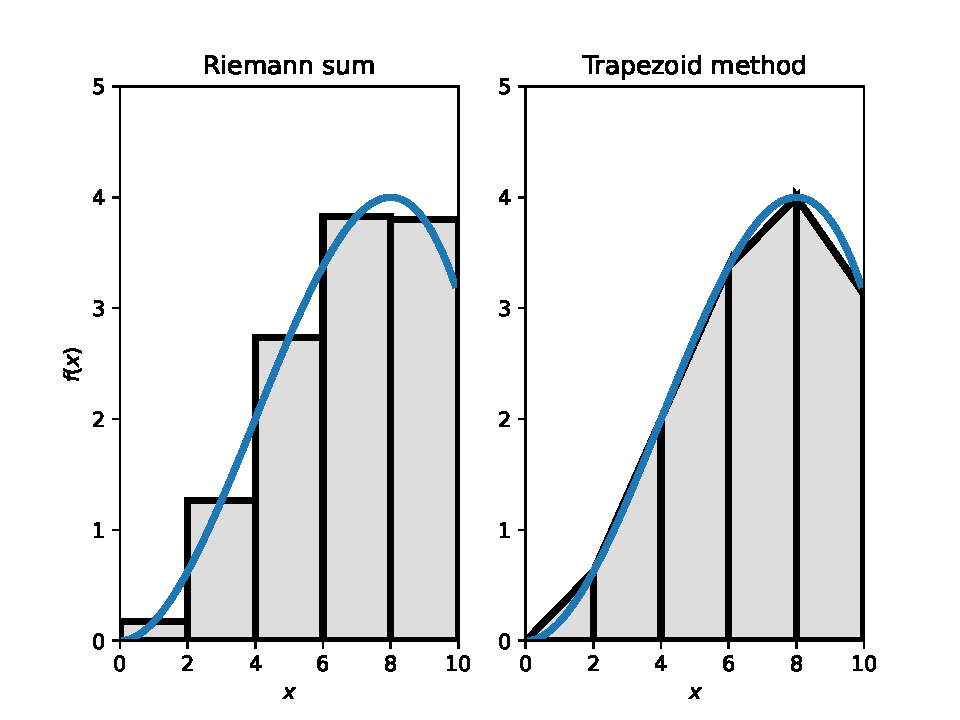
\includegraphics[height=12cm]{figs/plots/motion_classification/numericalintegration.pdf}
    \caption{Example function showcasing the differences in approximation accuracy between the Riemann sum method and the trapezoid method of numerical integration.}
    \label{fig:numericalintegration}
\end{figure}

The gradients computed by approximating the integral can now be used for training a neural network with gradient descent. What happens during training is that the parameters of the neural network starts to diverge towards infinity $|| \bm{\theta} || \rightarrow \infty$. The reason for this divergence is a result of the line integral loss function. If a neural network is trained with the L2 loss function $\frac{1}{n} \sum_{k=1}^{n} (y_k - \hat{y}_k)^2$, there exists a minimum value as a consequence of the fact that the function is nonnegative. The optimization problem proposed in (\ref{eq:lineintegralmax}) can be shown to be unbounded. Because $\bm{f}(t, \bm{r}_k(t); \bm{\theta})$ is represented with a neural network it can represent any function with enough parameters, which also means that the function can be decomposed as:

\begin{equation}
    \begin{aligned}
        & \bm{f} = \bm{f}_{\perp} + \bm{f}_{||} & \quad \\
        & \bm{f}_{\perp}(t, \bm{r}_k(t); \bm{\theta}) \cdot \bm{r}_k(t) = 0 & \quad \forall t \in \mathbb{R} \\
        & \bm{f}_{||}(t, \bm{r}_k(t); \bm{\theta}) = C(\bm{\theta}) \bm{r}_k(t) & \quad \forall t \in \mathbb{R} \\
    \end{aligned}
\end{equation}

\noindent for some function $C(\bm{\theta})$. Then $\bm{f} \cdot \bm{r}_k = \bm{f}_{\perp} \cdot \bm{r}_k + \bm{f}_{||} \cdot \bm{r}_k = C(\bm{\theta}) || \bm{r}_k ||^2$. The optimization problem becomes:

\begin{equation}
    \begin{aligned}
        \max_{\bm{\theta}} \quad & \frac{1}{n} \sum_{k=1}^{n} \int_{t_{k_0}}^{t_{k_1}} \bm{f} \cdot \bm{r}_k' dt & = & \frac{1}{n} \sum_{k=1}^{n} \int_{t_{k_0}}^{t_{k_1}} C(\bm{\theta}) || \bm{r}_k ||^2 dt \\
        & & = & C(\bm{\theta}) \frac{1}{n} \sum_{k=1}^{n} \int_{t_{k_0}}^{t_{k_1}} || \bm{r}_k ||^2 dt \\
        & & = & C(\bm{\theta}) K
    \end{aligned}
\end{equation}

\noindent where $K$ is a constant and therefore not relevant for the optimization problem. Because $C(\bm{\theta})$ can be any function expressed by a neural network, the optimization is unbounded.

A potential solution is to modify the optimization problem so that there is a well defined optimum. The dot product between two vectors $\bm{a}$ and $\bm{b}$ is given by the formula:

$$
\bm{a} \cdot \bm{b} = ||a|| ||b|| \cos(\angle{(\bm{a}, \bm{b})})
$$

If both vectors $\bm{a}$ and $\bm{b}$ have length $1$, the dot product simply becomes $\cos(\angle{(\bm{a}, \bm{b})})$ which always lie in the range $[-1, 1]$, with a maximum value of $1$ if $\bm{a}$ and $\bm{b}$ are pointing in the same direction. The problem can then be modified to by normalizing both $\bm{f}$ and $\bm{r}_k'$. The integral:

\begin{equation*}
    \int_{t_{k_0}}^{t_{k_1}} \frac{\bm{f}}{|| \bm{f} ||} \cdot \frac{\bm{r}_k'}{|| \bm{r}_k' ||} dt
\end{equation*}

\noindent will then have a maximum value of:

\begin{equation*}
    \int_{t_{k_0}}^{t_{k_1}} dt = t_{k_1} - t_{k_0}
\end{equation*}

\noindent when the vector field $\bm{f}$ perfectly aligns with $\bm{r}_k$ for all values of $t_{k_0} \leq t \leq t_{k_1}$. The normalized line integral loss function can then be formulated as:

\begin{equation}
    \mathcal{L} = - \frac{1}{n} \sum_{k=1}^{n} \frac{1}{t_{k_1} - t_{k_0}} \int_{t_{k_0}}^{t_{k_1}} \frac{\bm{f}(t, \bm{r}_k(t); \bm{\theta})}{|| \bm{f}(t, \bm{r}_k(t); \bm{\theta}) ||} ^T \frac{\bm{r}_k'(t)}{|| \bm{r}_k'(t) ||} dt
    \label{eq:normalizedlineintegral}
\end{equation}

\noindent with a minimum value of -1 if $\bm{f}$ perfectly aligns with all the trajectories in the training set.

The gradients can be computed in a similar method as the line integral without normalization:

\begin{equation}
    \begin{aligned}
        \frac{\partial \mathcal{L}}{\partial \bm{\theta}}
        & = - \frac{\partial}{\partial \bm{\theta}} \begin{bmatrix} \frac{1}{n} \sum_{k=1}^{n} \frac{1}{t_{k_1} - t_{k_0}} \int_{t_{k_0}}^{t_{k_1}} \frac{\bm{f}(t, \bm{r}_k(t); \bm{\theta})}{|| \bm{f}(t, \bm{r}_k(t); \bm{\theta}) ||} ^T \frac{\bm{r}_k'(t)}{|| \bm{r}_k'(t) ||} dt \end{bmatrix} \\
        & = - \frac{1}{n} \sum_{k=1}^{n} \frac{1}{t_{k_1} - t_{k_0}} \int_{t_{k_0}}^{t_{k_1}} \frac{\partial}{\partial \bm{\theta}} \begin{bmatrix} \frac{\bm{f}(t, \bm{r}_k(t); \bm{\theta})}{|| \bm{f}(t, \bm{r}_k(t); \bm{\theta}) ||} ^T \frac{\bm{r}_k'(t)}{|| \bm{r}_k'(t) ||} \end{bmatrix} dt \\
        & = - \frac{1}{n} \sum_{k=1}^{n} \frac{1}{t_{k_1} - t_{k_0}} \int_{t_{k_0}}^{t_{k_1}} \frac{\bm{r}_k'(t)}{|| \bm{r}_k'(t) ||}^T \frac{\partial}{\partial \bm{\theta}} \begin{bmatrix} \frac{\bm{f}(t, \bm{r}_k(t); \bm{\theta})}{|| \bm{f}(t, \bm{r}_k(t); \bm{\theta}) ||} \end{bmatrix} dt \\
    \end{aligned}
\end{equation}

Computing the partial derivative $\frac{\partial}{\partial \bm{\theta}} \begin{bmatrix} \frac{\bm{f}(t, \bm{r}_k(t); \bm{\theta})}{|| \bm{f}(t, \bm{r}_k(t); \bm{\theta}) ||} \end{bmatrix}$ can be done by first using the formula for differentiating a normalized vector \citep{matrixcookbook}:

\begin{equation}
    \frac{\partial}{\partial \bm{x}} \frac{\bm{x} - \bm{a}}{|| \bm{x} - \bm{a} ||}
    = \frac{\bm{I}}{|| \bm{x} - \bm{a} ||} - \frac{(\bm{x} - \bm{a}) (\bm{x} - \bm{a})^T}{|| \bm{x} - \bm{a} ||^3}
\end{equation}

\noindent with $\bm{a} = 0$. Then by using this formula combined with the chain rule results in:

\begin{equation}
    \begin{aligned}
        \frac{\partial}{\partial \bm{\theta}} \frac{\bm{f}}{|| \bm{f} ||}
        &= \begin{bmatrix} \frac{\partial}{\partial \bm{f}} \frac{\bm{f}}{|| \bm{f} ||} \end{bmatrix} \frac{\partial \bm{f}}{\partial \bm{\theta}} \\
        &= \begin{bmatrix} \frac{\bm{I}}{|| \bm{f} ||} - \frac{\bm{f} \bm{f}^T}{|| \bm{f} ||^3} \end{bmatrix} \frac{\partial \bm{f}}{\partial \bm{\theta}}
    \end{aligned}
\end{equation}

The final gradient is then expressed as:

\begin{equation}
    \begin{aligned}
        \frac{\partial \mathcal{L}}{\partial \bm{\theta}} = - \frac{1}{n} \sum_{k=1}^{n} \frac{1}{t_{k_1} - t_{k_0}} \int_{t_{k_0}}^{t_{k_1}} \frac{\bm{r}_k'}{|| \bm{r}_k' ||}^T \begin{bmatrix} \frac{\bm{I}}{|| \bm{f} ||} - \frac{\bm{f} \bm{f}^T}{|| \bm{f} ||^3} \end{bmatrix} \frac{\partial \bm{f}}{\partial \bm{\theta}} dt
    \end{aligned}
\end{equation}

\noindent where the integral can be approximated using trapezoid integration. It is also worth noting that if all the trajectories have the same start time $t_0$ and end time $t_1$, the gradient simplifies to:

\begin{equation}
    \begin{aligned}
        \frac{\partial \mathcal{L}}{\partial \bm{\theta}} = - \frac{1}{n} \frac{1}{t_1 - t_0} \int_{t_0}^{t_1} \sum_{k=1}^{n} \frac{\bm{r}_k'}{|| \bm{r}_k' ||}^T \begin{bmatrix} \frac{\bm{I}}{|| \bm{f} ||} - \frac{\bm{f} \bm{f}^T}{|| \bm{f} ||^3} \end{bmatrix} \frac{\partial \bm{f}}{\partial \bm{\theta}} dt
    \end{aligned}
\end{equation}

\noindent by swapping the integral and summation. This is often useful for vectorization purposes in implementations, which can give a significant speedup.

The adjoint method for Neural ODEs can be used in a black box optimization setting, which means that it is easier to train Neural ODEs as single components of a larger model. Because this loss function works directly on the vector field and trajectories it does not allow the same level of flexibility in model design, so the trained vector field can not be used for representation learning in the same way. This makes the loss function less useful than the standard adjoint method with any loss function for most purposes. Additionally, the line integral will only make sense to compute when the dynamics are learned directly. For example will Augmented Neural ODEs increase the dimension in a way that does not easily map back to the dimension of the data trajectories. Simply ignoring the extra dimensions and computing the line integral will not reflect the true behavior of the learned system.

To see how well the normalized line integral works as a loss function, train a model on the mass spring damper system. Also train a regression model and a standard Neural ODE for comparison. For all three models, compute the L2 loss on integrated trajectories and also the normalized line integral loss over the validation set. Use the values $h=0.01$ and $T=1$. The results are displayed in Figure \ref{fig:line_integral_comparison_no_k}. The model trained with the line integral loss has the best performance in terms of the normalized line integral, but has poor performance when looking at the integrated trajectories.

\begin{figure}[H]
    \centering
    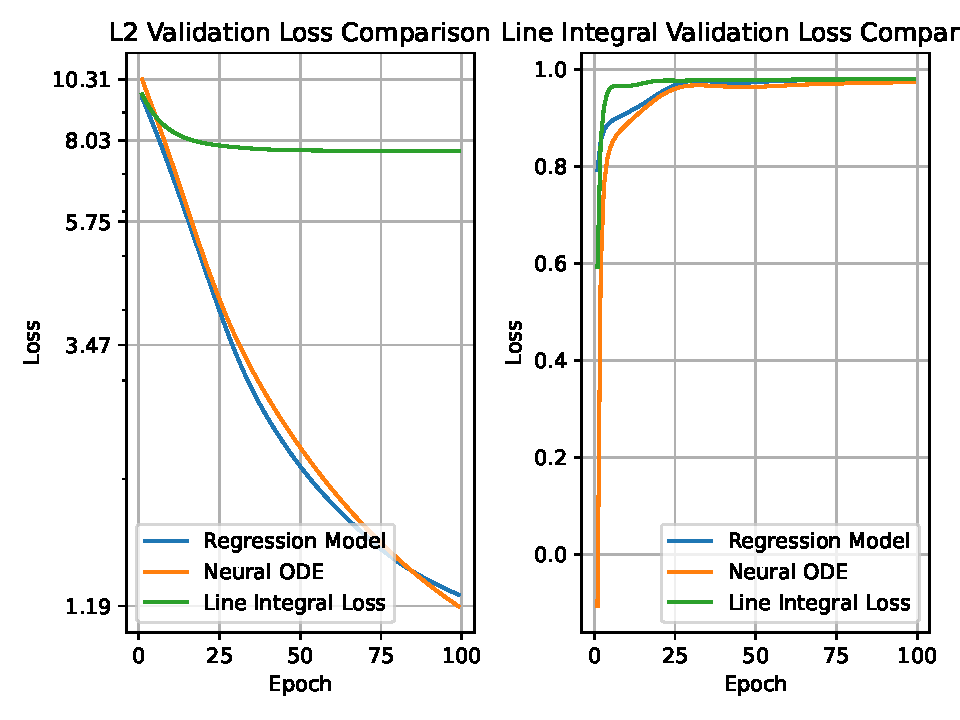
\includegraphics[height=10cm]{figs/plots/motion_classification/line_integral_comparison_no_k.pdf}
    \caption{Regression Model, Neural ODE and a model trained with the line integral loss on the mass spring damper.}
    \label{fig:line_integral_comparison_no_k}
\end{figure}

The explanation for this is that the model learns the orientation of the underlying vector field, but fails to capture the magnitude. This phenomenon is a consequence of the normalization in the line integral loss. A potential solution is to create a second neural network which learns the magnitudes of the trajectories. The output from this neural network can then be multiplied with the output of the line integral model and used as a scaling factor. The end result is basically a more convoluted regression model. An alternative and simpler solution is to instead represent the scaling as a simple constant which can be multiplied with the line integral model output. If $\bm{f}$ is the output from the model, the constant scaling factor $C$ can be defined as:

\begin{equation}
    C = \frac{1}{n} \sum_{k=1}^n \frac{1}{m_k} \sum_{j=1}^{m_k} \frac{|| \bm{r}_{k j} ||}{|| \bm{f}(\bm{r}_{k j}) ||}
\end{equation}

\noindent by averaging over the trajectories in the training set. Each trajectory $\bm{r}_k(t)$ is discretized into $m_k$ samples indexed by $j$. To save some computational time it is also possible to use some randomly chosen trajectories instead of the whole set.

Adding the scaling factor $C$ and training the models again can be seen below in Figure \ref{fig:line_integral_comparison_with_k}. The training duration is also increased to 300 epochs.

\begin{figure}[H]
    \centering
    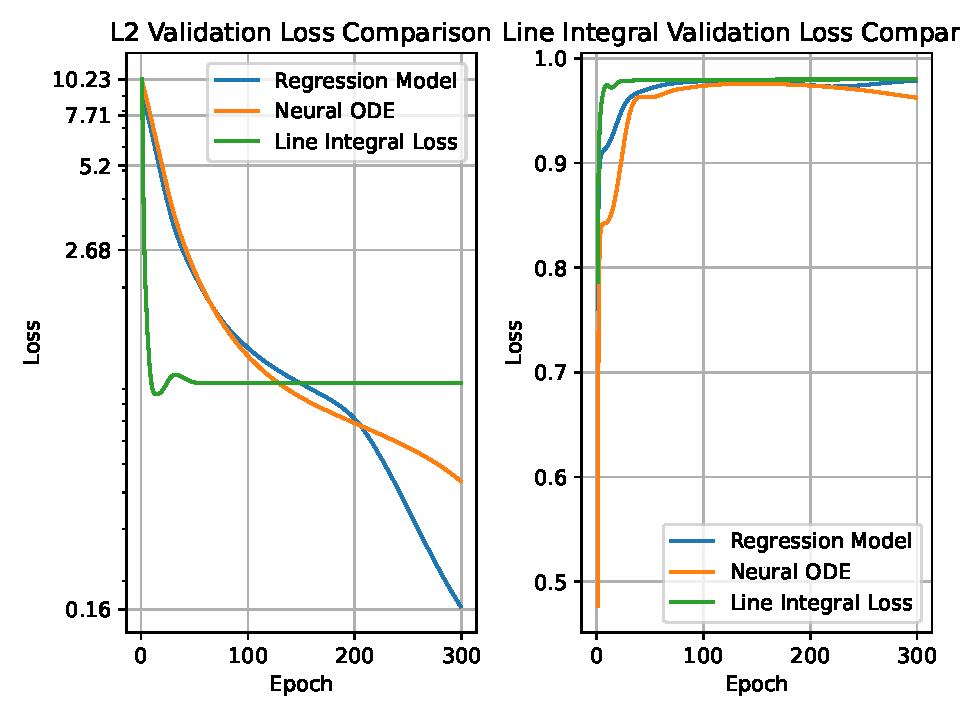
\includegraphics[height=10cm]{figs/plots/motion_classification/line_integral_comparison_with_k.pdf}
    \caption{Regression Model, Neural ODE and a model trained with the line integral loss on the mass spring damper. The line integral model is multiplied with a constant when used for integration.}
    \label{fig:line_integral_comparison_with_k}
\end{figure}

The line integral model learns the orientation of the underlying vector field just as quickly as without the scaling factor. The scaling factor is able to approximate the underlying dynamics to a certain extent, but the training will converge relatively fast. It is therefore better than the regression model and Neural ODE at first, but the other two models will eventually perform better after enough training epochs.

For a linear system on the form $\dot{\bm{x}} = \bm{A} \bm{x}$ where $\bm{A}$ is a square matrix, the magnitude of the dynamics becomes:

\begin{equation*}
    || \dot{\bm{x}} || = ||\bm{A} \bm{x}|| \leq ||\bm{A}|| ||\bm{x}||
\end{equation*}

\noindent which essentially means that the magnitude is dependent on the distance from the origin. The constant scaling factor $C$ will then only give an approximating of the true system magnitudes, which is very dependent on the available training data. To explore whether this approximation can work for nonlinear systems with a more complex magnitude, also train the three models on the pendulum dynamics. The results are displayed below in Figure \ref{fig:line_integral_comparison_with_k_pendulum} with the scaling factor.

\begin{figure}[H]
    \centering
    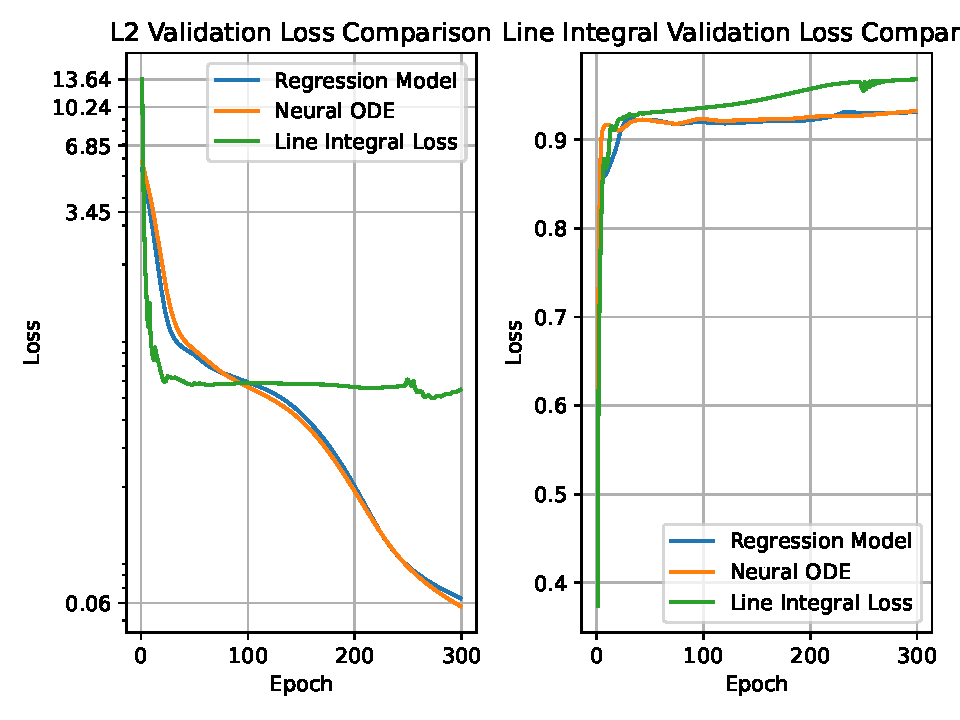
\includegraphics[height=10cm]{figs/plots/motion_classification/line_integral_comparison_with_k_pendulum.pdf}
    \caption{Regression Model, Neural ODE and a model trained with the line integral loss on the pendulum. The line integral model is multiplied with a constant when used for integration.}
    \label{fig:line_integral_comparison_with_k_pendulum}
\end{figure}

The result on the nonlinear system is very similar to the linear system, in that the line integral model learns the orientation of the dynamics very fast, with higher performance than the other two models. When it comes to integrating trajectories, the line integral model does not manage to do this well compared to the other models, even with a scaling factor.

To conclude, training models to learn dynamical systems with the normalized line integral loss function can work depending on the goal of the model. If the goal is to accurately simulate the system the line integral will not give accurate results. However, when the orientation of the vector field is the only thing that matters, the line integral loss will be a much more efficient method. This will be used in the next section.

\section{Classification with Line Integrals}

Assume now that the basic motion classification framework consists of two different dynamical systems, with training data containing trajectories in the form of time-series sampled from both of these systems. The proposed classification algorithm uses the fact that the normalized line integral (\ref{eq:normalizedlineintegral}) always gives a value in the range $(-1, 1)$. This can be used to measure how well a given trajectory aligns with a vector field. If the two dynamical systems have known differential equations, a simple classification algorithm can then be to compute the line integral of a given trajectory over both versions, and then see which system has the highest value of the line integral. However, if the differential equations are assumed unknown it is possible to train a Neural ODE model for each class, and then see which trained model aligns the best with a given trajectory. If the two trained models learn the true dynamics well enough they should give similar results to using the true systems directly for computing the line integrals. Because the line integrals are normalized it also means that the magnitudes of the trained dynamics are insignificant, so the two models can be trained with the line integral loss as described in the previous section.

To further increase the robustness of the classification algorithm, instead of simply checking which of the models gives the highest value of the line integral, the two computed line integrals can be considered as new features for a separate classification algorithm. A given trajectory will then generate two new features, one line integral for each trained model. More sophisticated classification algorithms can be trained on trajectories with the given line integral features. The full classification algorithm then becomes training separate Neural ODE models with the line integral loss for each class of dynamics, and then afterwards training a separate classification algorithm on line integrals computed from the Neural ODE models. This approach with a separate classification algorithm can also be naturally extended to more than two classes.

In some cases there could be an imbalance in the dataset with much more available training data for one of the classes. In this case it could make sense to phrase it as an anomaly detection problem by only training a Neural ODE on one of the classes. Line integrals computed on new trajectories will still give a value depending on how well it aligns with the vector field. A classification algorithm can then be to find a threshold value and classify everything over the threshold as belonging to the class the model was trained on. This method does not work with more than two classes, and is most likely less useful when there is enough data to train separate models.

\section{Experimental Setup}

To test the proposed classification algorithms, consider the double pendulum dynamical system. Double pendulums are chaotic systems in four dimensions which means they are more difficult to learn than the single pendulum. Another motivation for choosing double pendulums is that they can be used as a simplified model of a human limb which can be useful for medical applications, for example when it comes to detecting and diagnosing movement issues.

The first version of the double pendulum to be used is the unconstrained free moving system. The ODE that describes this dynamical system can be derived with Lagrangian mechanics and results in the following expression:

\begin{adjustwidth}{-2cm}{-2cm}
    \begin{equation}
        \frac{d}{d t} \begin{bmatrix} \theta_1 \\ \theta_2 \\ \dot{\theta}_1 \\ \dot{\theta}_2 \end{bmatrix}
        = \begin{bmatrix}
            \dot{\theta}_1 \\ \dot{\theta}_2 \\ 
            \begin{bmatrix}
                (m_1 + m_2) l_1^2 & m_2 l_1 l_2 \cos(\theta_1 - \theta_2) \\
                m_2 l_1 l_2 \cos(\theta_1 - \theta_2) & m_2 l_2^2
            \end{bmatrix}^{-1}
            \begin{bmatrix} -m_2 l_1 l_2 \sin(\theta_1 - \theta_2) \dot{\theta}_2^2 - (m_1 + m_2) g l_1 \sin{\theta_1} \\ m_2 l_1 l_2 \sin(\theta_1 - \theta_2) \dot{\theta}_1^2 - m_2 g l_2 \sin{\theta_2}\end{bmatrix}
        \end{bmatrix}
        \label{eq:doublependulumequation}
    \end{equation}
\end{adjustwidth}

The full derivation of the double pendulum dynamics can be viewed in Appendix \ref{appendix:doublependiulumdynamics}.

\begin{figure}[H]
    \centering
    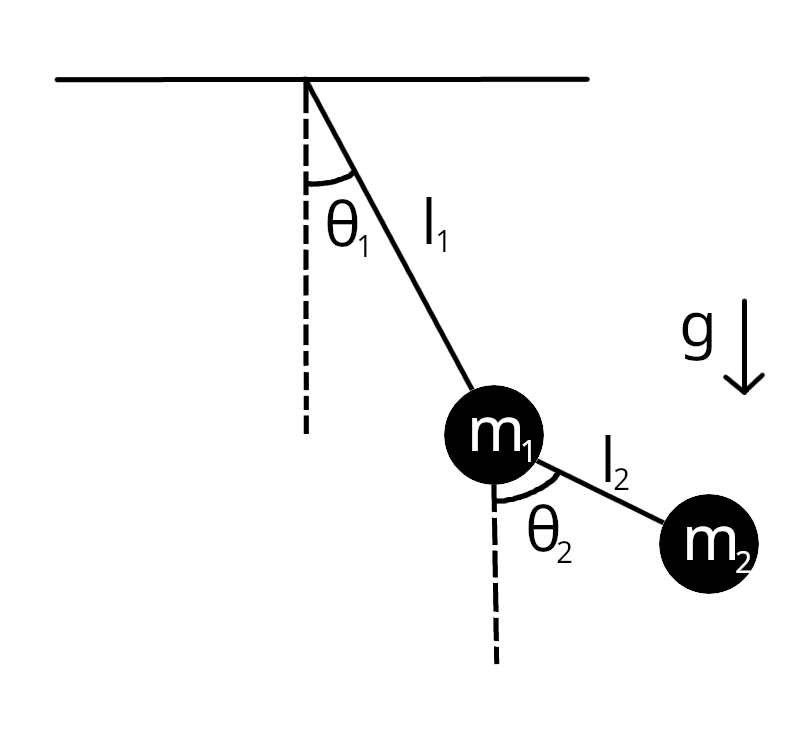
\includegraphics[height=8cm]{figs/doublependulum.png}
    \caption{Double pendulum system.}
    \label{fig:doublependulum}
\end{figure}

The second version of the double pendulum to be used is obtained by adding constraints to limit the movement. Because adding true constraints is not so obvious with Lagrangian mechanics, the constraints are instead treated more like soft constraints instead of hard constraints of the system. This is achieved by adding a torque to the second link when the angle difference between the first and the second link gets too large. To make this behavior work continuously, a PD controller is added that drives the second link towards the first. A PD (Proportional Derivative) controller is a mathematical expression that creates an input signal (torque in this case) that makes the system follow a reference signal. The first link $\theta_1$ is driven towards the origin very slowly, and the second link $\theta_2 $is driven towards $\theta_1$ more rapidly. The expression was in this case chosen to be:

\begin{equation}
    \begin{aligned}
        u_1 &= -0.001 \theta_1 - 0.001 \dot{\theta_1} \\
        u_2 &= -1 (\theta_2 - \theta_1) - 0.5 \dot{\theta_2}
    \end{aligned}
\end{equation}

\noindent where $\bm{u} = \begin{bmatrix} 0 & 0 & u_1 & u_2 \end{bmatrix}^T$ is the input signal to the dynamical system and is added to the RHS of (\ref{eq:doublependulumequation}). These two versions of the double pendulum are relatively similar to each other and will in many cases have indistinguishable trajectories. For example, if the initial condition of the systems is at the origin, meaning the double pendulum is hanging straight down with zero velocity, the two systems will have the same trajectory (remaining at the origin). This can have some impact in regards to classification performance.

The training and validation data is generated from the two double pendulums by sampling random initial values uniformly. The different states of the initial values are sampled differently. The first state corresponding to the angle $\theta_1$ is sampled in the range $(-3 , 3)$, which is approximately within 180 degrees in either rotation. The second angle $\theta_2$ is set to the value of $\theta_1$ plus a randomly sampled value in the range $(-0.5, 0.5)$. The angular velocities are sampled in the ranges $(-2, 2)$ and $(-1, 1)$. 200 initial values are sampled to both the training and validation sets. These initial values are then integrated using the two versions of the double pendulum to produce 200 trajectories for each double pendulum version and for both the training and validation set. In total, 800 trajectories are generated.

To measure performance and usefulness of the proposed classification algorithms they will be compared to a baseline model. In this case, the baseline model consists of LSTM with a classifier head. The LSTM architecture is a type of Recurrent Neural Network (RNN) that also models connections between elements in a sequence. RNNs will often achieve better performance than standard ANNs on time-series due to the sequential structure. The baseline model uses 300 hidden units in the LSTM. The classifier head takes the final hidden state of the LSTM as input and consists of two fully connected layers with 300 and 150 nodes, and the sigmoid activation function after both layers. As the double pendulum setup described above has two classes it is a binary classification problem, so the classifier head has an output dimension of 1, with values in the range $(0, 1)$ due to the sigmoid function.

Use the true system equations to compute line integrals averaged over the training set. For the anomaly detection setup, these values can be used to determine which of the two versions would be the most useful to base a classifier from. Then two classification algorithms are trained on features generated from the true system. The first is the logistic regression model, which is one of the simpler binary classification algorithms, and will essentially find a threshold for the classification. The second is a Support Vector Machine (SVM), which is more sophisticated than the logistic regression, but still relatively simple compared to a random forest model or a neural network.

Afterwards, replace the true systems with models trained with the line integral loss. One model is trained for each version of the pendulum. Both of the trained models contain six fully connected layers with the $\tanh$ activation function between layers. The layers contain 4, 50, 100, 200, 100 and 50 nodes in that order, with 4 as the output dimension. Use the best of the classification algorithms found with the true systems to determine the potency of the anomaly detection setup. For the purpose of training the classifier, the previous validation set is split into two sets, one for training the classifier and the other for validating it. This ensures that the classifier is trained on separate data from the Neural ODE models. Finally, use the classification algorithm trained on features from both trained models together.

\section{Results}

The training process of the LSTM baseline is shown in Figure \ref{fig:lstm_acc}. After 200 epochs the model reaches a classification accuracy of $98 \%$ on the validation set. As the baseline is not particularly tuned, it might be possible to increase this accuracy to $100 \%$ with some hyperparameter optimization. This could be an indication that the overall problem is too simple, although it is still useful to see if the algorithm with line integrals is able to give a similar performance.

\begin{figure}[H]
    \centering
    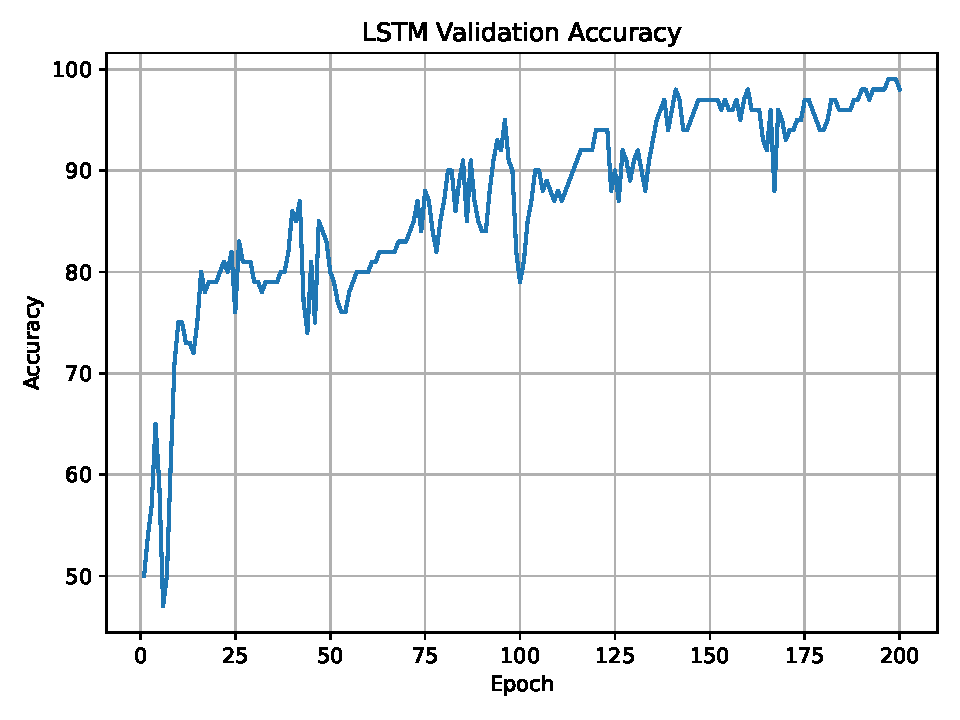
\includegraphics[height=12cm]{figs/plots/motion_classification/lstm_acc.pdf}
    \caption{LSTM classification accuracy on the validation set during training.}
    \label{fig:lstm_acc}
\end{figure}

The result from computing the normalized line integrals for the true system is displayed in Table \ref{tab:integrals}. Both the unconstrained and constrained true systems are used with the full training data divided into trajectories generated from the unconstrained and constrained systems. The constrained model has the largest difference between the line integrals, which could indicate that this is the model to use for the easiest classification. The averaged line integrals for the batch from the same model would be expected to be equal to 1 exactly, but are instead 0.970 and 0.973. The difference could be because of numerical errors, and particularly because the derivatives used for calculating the line integrals are approximated with finite differences and using a value of h = 0.1. The integrals are also approximated using the trapezoid method which also slightly reduces the accuracy.

\begin{table}[H]
    \centering
    \caption{Normalized line integrals computed for the two versions of the double pendulum using the true systems. Integrals are averaged over the whole training set.}
    \begin{tabular}{|c | c | c|} 
        \hline
        & Unconstrained data & Constrained data \\
        \hline
        Unconstrained system & 0.970 & 0.913 \\
        \hline
        Constrained system & 0.743 & 0.973 \\
        \hline
    \end{tabular}
    \label{tab:integrals}
\end{table}

Training the two classifiers on line integral features computed with the true systems resulted in the validation accuracies in Table \ref{tab:true_accs}. The SVM achieved $100 \%$ validation accuracy on the constrained system, which indicated that it is able to better learn to differentiate the values. Overfitting is possible, but also unlikely as the validation data has not been seen during training.

\begin{table}[H]
    \centering
    \caption{Validation accuracy of the two classification algorithms using line integrals computed from one model.}
    \begin{tabular}{|c | c | c|} 
        \hline
        & Logistic Regression & SVM \\
        \hline
        Unconstrained system & $83 \%$ & $98 \%$ \\
        \hline
        Constrained system & $76 \%$ & $100 \%$ \\
        \hline
    \end{tabular}
    \label{tab:true_accs}
\end{table}

The true systems was now replaced with Neural ODEs trained with the line integral loss. Table \ref{tab:true_accs} could indicate that training a model on trajectories generated from the constrained system with the SVM classifier would be the best approach, but both versions were used for comparison with their own separate classifiers. The SVM classifier was also trained from scratch each epoch. This was not strictly necessary as it would have been enough to train the SVM once after the models were fully trained, but training each epoch shows the progression more clearly. The classification accuracies during training are displayed in Figure \ref{fig:line_integral_singlemodel_acc}. As indicated by Table \ref{tab:true_accs}, the constrained model achieves the best accuracy with the SVM at $84 \%$. As the SVM based on the true system achieved $100 \%$ it could indicate that the models are not able to perfectly learn the double pendulums.

\begin{figure}[H]
    \centering
    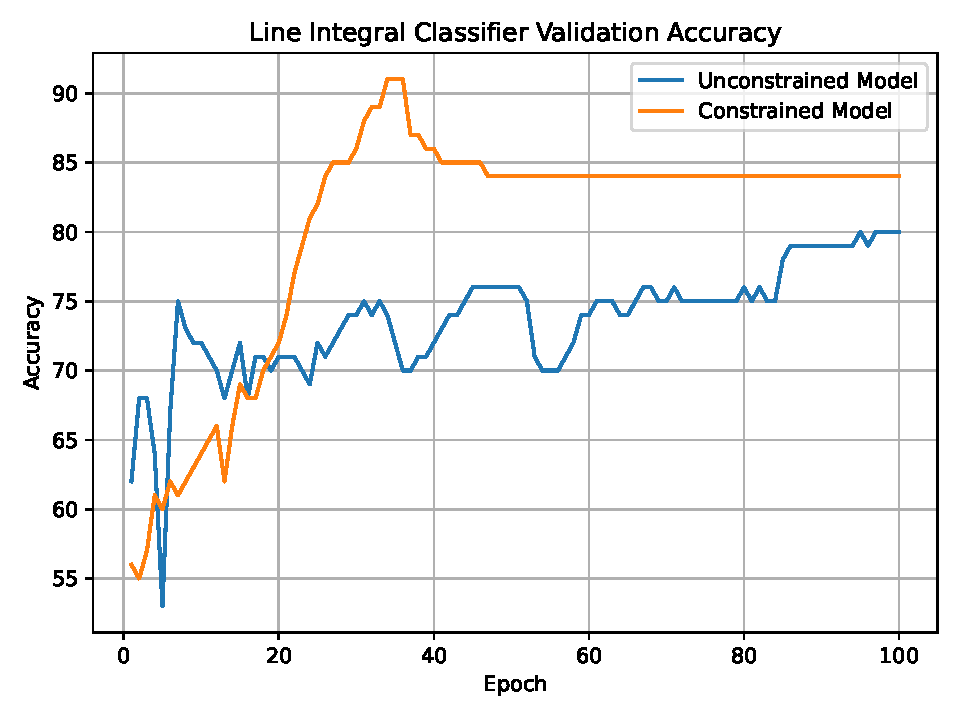
\includegraphics[height=12cm]{figs/plots/motion_classification/line_integral_singlemodel_acc.pdf}
    \caption{SVM classifier trained on line integrals from one of the models. Displays the classification accuracy on the validation set during training.}
    \label{fig:line_integral_singlemodel_acc}
\end{figure}

The final results from training one SVM classifier with two features computed from both trained models are shown in Figure \ref{fig:line_integral_doublemodel_acc}. The SVM manages to achieve a validation accuracy of $100 \%$ after 100 epochs of training. Even though the trained models are not able to perfectly capture the double pendulum dynamics the combined line integrals make it possible to distinguish the two classes. The proposed algorithm is then able to slightly outperform the LSTM baseline model in half the number of epochs.

\begin{figure}[H]
    \centering
    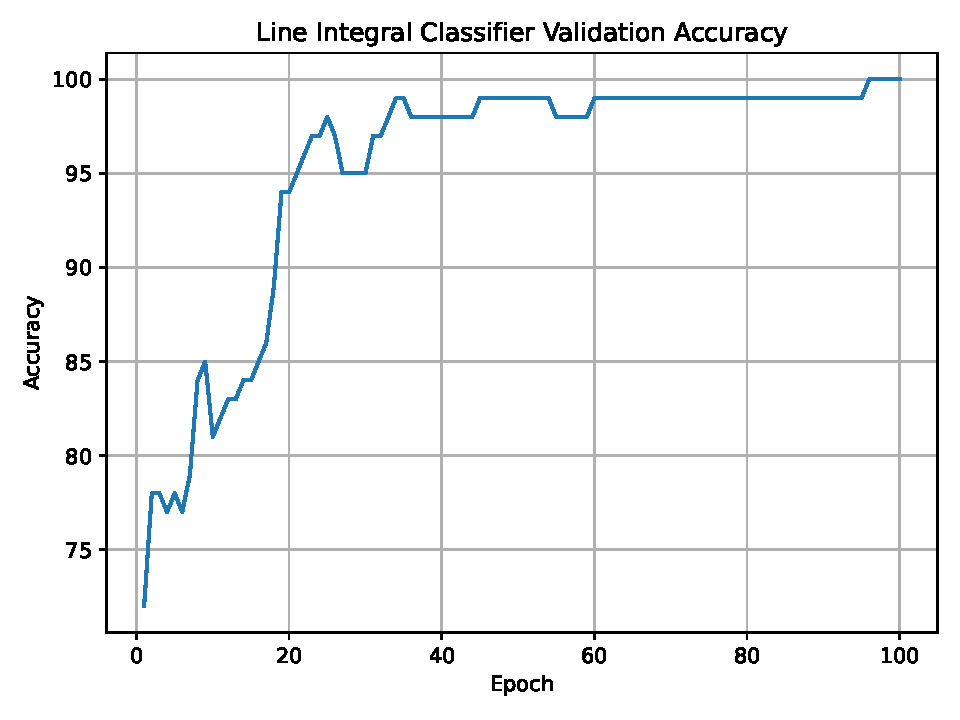
\includegraphics[height=12cm]{figs/plots/motion_classification/line_integral_doublemodel_acc.pdf}
    \caption{SVM classifier trained on line integrals from both models. Shows the classification accuracy on the validation set during training.}
    \label{fig:line_integral_doublemodel_acc}
\end{figure}

\chapter{Conclusion}
\label{cha:conclusion}

This final chapter discusses the proposed method for motion classification as well as the overall contributions of the work from this thesis. It also brings up some potential future work to address shortcomings and further improve the method.

\section{Discussion}
\label{sec:Discussion}

The overall goal of this thesis was to use the Neural ODE model for motion classification tasks. The assumption that motions are generated by dynamical systems motivates the use of Neural ODE and exploits the inductive bias where a dynamical system is a part of the internal architecture of the model.

The results from chapter \ref{cha:learningdynamicalsystems} shows that the Neural ODE architecture is able to learn representations for dynamical systems. The architecture also has the additional property that it can work with much more sparsely sampled data than a simple regression model. It also highlighted some of the shortcomings in the original model and implemented an improved version of the model to compensate for these issues.

Chapter \ref{cha:motionclassification} then derives a method for generating features based on the line integral from vector calculus which gives a score of how well a trajectory aligns with a vector field. Chapter \ref{cha:motionclassification} also shows that it is possible to use the line integral as a loss function directly, and train models using gradients derived from the line integral. The line integral was modified to add normalization on both the vector field and trajectory derivatives to avoid unboundedness. An alternative strategy for dealing with the unboundedness is to add regularization on the parameters, although the parameters might still not converge to the correct values for representing the underlying system.

The results from training on the normalized line integral loss shows that such models outperforms both standard Neural ODE models and regression models when it comes to learning the orientation of the vector field, as it both learns faster and achieves higher performance. The results also show that the line integral model is less useful for simualating systems as the magnitudes are not accurate. Adding a constant scaling factor calculated from the true derivatives was also not useful in correcting this.

The overall implication is that training models with the line integral loss is not useful in the general case, as they also need access to the derivatives of the trajectory. Another drawback of the line integral loss model is that it does not currently contain expressions for calculating gradients from the loss to the input, as it is not obvious how to do it considering that a whole multi-dimensional trajectory must be considered as one input. This makes it impossible to use the model as a part of a single larger model as it is not possible to have models that transform the input first or transform the output afterwards.

Although training with the line integral loss is not so useful for learning a dynamical system accurately, nor is it useful as a deep model for representation learning, it can still be useful for classification. Using normalized line integrals as feature generation for a separate classifier model means that the magnitude of the vector field is irrelevant, which means that training with the normalized line integral loss directly can speed up the overall training process.

The results from using the real systems for calculating line integrals showed that it was possible to use a simple classification algorithm to distinguish the systems, although one model was required for each class of dynamics. Using just one system with a classifier was not enough to get perfect accuracy which means that for systems with relatively similar dynamics there can be some trajectories that are indistinguishable. Sampling trajectories for a longer time period can help mitigate these issues as the small differences would accumulate over longer intervals.

One issue that can arise is when one of the systems to classify is a scaled version of the other. In this case, the normalized line integrals will always return the same values as the two systems have vector fields with identical orientations. The proposed method will not work here, but the classification problem can also be trivially solved by simply finding the velocities of a trajectory and checking which system it then matches.

For the two double pendulum systems the Neural ODEs trained with the normalized line integral loss did eventually learn the system orientation well enough to achieve a $100 \%$ classification accuracy with an SVM for the classification part. This shows that the proposed model can work for classification, as long as the trained models are able to learn the true dynamics accurately enough. As the double pendulum is relatively complex and chaotic it could make sense to use the Lagrangian Neural Network model. The normalized line integral loss is not directly applicable for training but can still be used for computing features for the classifier.

The double pendulum dynamics are only four dimensional, so it remains to be seen if the proposed classification algorithm also can work for more complex systems with higher dimensionalities. Many real life systems must also be considered as time-dependent due to being controlled by external signals. The normalized line integral can still be computed in the same way but the trained dynamic models must take the time-dependency into account.

\section{Contributions}
\label{sec:Contributions}

The first research question asks what the current state of the art Neural ODEs is. A presentation of many of the most significant improvements to the original model by \cite{node} were given in chapter \ref{cha:sota}. These improvements include the direct extensions originating with the Augmented Neural ODE model by \cite{dupont2019augmented} and the generalized framework presented by \cite{massaroli2021dissecting} for constructing a Neural ODE based model. These additions both increase the representative abilities of Neural ODEs as well as improving the training performance. Other models that forced the dynamics to take a certain form includes the Hamiltonian model by \cite{hamiltoniannode}, the Lagrangian model from \cite{lagrangiannode} and the stable neural flow model by \cite{stableneuralflows} which can be situationally useful for learning dynamical systems on a specific form. The time-dependent model of \cite{timedependencenode} further increases the representable class of functions and can also be situationally useful. Increasing robustness through stochastic modeling was made feasible by the backward algorithm proposed by \cite{sdegradients}.

The second research question asked about how properties of the dataset affects the model choice. If it is possible to compute derivatives of the true underlying system and if the sample interval is low enough, the derivatives can be approximated and used for training a regression model. For these cases a Neural ODE model is less useful. But for sample intervals too high to make meaningful approximations, it does not make sense to use regression models. If the sample interval is non-constant it can also make the same derivatives take different values depending on where they were sampled from. For these cases Neural ODEs will vastly outperform regression models, being possible to train with much less datapoints in a trajectory. The augmented variant is also capable of learning systems not possible to represent as a regression model.

The last research question was about how useful Neural ODE based models are for motion classification tasks. The answer to this research question is also the main contribution of this master thesis. Through the use of generating features from a line integral of the learned vector field and a trajectory it is possible to train a separate classifier on these features. This method gives results on par with a baseline model, and can easily be extended to handle multiple classes.

\section{Future Work}
\label{sec:futureWork}

By using the real system dynamics directly to generate features for the classifier it was easy for the classifier to learn the differences between the two double pendulum versions. This means that if a Neural ODE based model is able to learn the true system dynamics well enough it can be substituted in and still achieve good classification performance. A possible improvement to training a model with the line integral loss is then to use a Lagrangian Neural Network for training on the double pendulum trajectories. The line integral can still be computed using equation (\ref{eq:lagrangianmechanicssolved}) to represent the vector field of the integral. The Hamiltonian model is not as practical for the double pendulum as the momentum coordinates which would be necessary for training are not computable without also knowing the parameters of the underlying dynamics.

A method for increasing the general accuracy of the model trained with the line integral loss is to train a separate neural network for representing the scaling factor. Instead of simply averaging out over the trajectories, the scaling can be defined as: $C = \bm{g}(t, \bm{x})$ with a neural network representing $\bm{g}$. Training $C$ is very similar to training the regression model with target values equal to $|| \bm{f}(t, \bm{x}) ||$. This training method involving two models will then have one model for learning the orientation of the vector field and a second model for learning the magnitude, decoupling the learning process. It was shown that the line integral loss resulted in a model that learned the orientation much faster than the other two methods, and it might be possible to perform regression when the target output is a scalar instead of the full vector.

Another experiment to further test the validity of the line integrals is to try with more than two classes. The feature generation will still work in the same way, where each feature is computed from a line integral over each trained Neural ODE model. It might also be necessary to use more sophisticated classification algorithms than a simple SVM. Ensemble algorithms based on decision tree classifiers often work well on tabular data. A classification model can also be constructed using neural networks. The stable neural flow model can also be used for classification on the line integral features. It might be possible to come up with a classification method based on the stable neural flow model that works for whole trajectories and not just single datapoints.

Adding random noise to data generation in the conducted experiments should also be attempted, as real sensors usually contain some noise. The added noise might make it so the training with the line integral loss no longer works due to overfitting on the noise realization, but that remains to be tested. The Neural ODE models could also be replaced with stochastic variants. It could also be possible to incorporate the stochastic robustness properties into other models like the Lagrangian Neural Network model or make the line integral loss work with stochastic dynamics.

The LSTM baseline model was able to achieve good results when classifying the two versions of the double pendulum. This could indicate that the problem is too easy to use as a meaningful test of the proposed method with line integrals. The new method should then be tested on much higher dimensional systems where it is much more difficult to separate the classes with traditional methods.

A final note to bring up is that if a stable neural flow model is used with resulting in dynamics of the form:

\begin{equation}
    \dot{\bm{x}} = \nabla f(\bm{x})
    \label{eq:stableflowequation}
\end{equation}

\noindent with $f(\bm{x})$ represented as a neural network with a scalar output, it is possible to greatly simplify the computation of line integrals. It is known from vector calculus that the line integral of a vector field $\nabla f(\bm{x})$ over a curve $\Gamma$ can be computed as:

\begin{equation}
    \int_{\Gamma} \nabla f(\bm{r}) \cdot d \bm{r} = f(\bm{r}(t_1)) - f(\bm{r}(t_0))
\end{equation}

\noindent when $f(\bm{x})$ is scalar. A consequence of this is that the line integral only depends on the start and end points, and is independent of the path. This also implies that the line integral will be zero for any curve with the same start and end point, which further implies that periodic trajectories are impossible to learn with this setup.

Training a model on the form of (\ref{eq:stableflowequation}) with the line integral results in the following expression:

\begin{equation}
    \begin{aligned}
        \mathcal{L}
        &= - \frac{1}{n} \sum_{k=1}^{n} \frac{1}{t_{k_1} - t_{k_0}} \int_{t_{k_0}}^{t_{k_1}} \begin{bmatrix} \nabla f(\bm{r}_k) \end{bmatrix}^T \bm{r}_k' dt \\
        &= - \frac{1}{n} \sum_{k=1}^{n} \frac{1}{t_{k_1} - t_{k_0}} \begin{bmatrix} f(\bm{r}_k(t_{k_1})) - f(\bm{r}_k(t_{k_0})) \end{bmatrix}
    \end{aligned}
    \label{eq:lineintegralstableflow}
\end{equation}

\noindent which has the advantage over the standard line integral loss that it can be computed without having explicit access to the derivatives $\bm{r}'(t)$ and that the line integral itself and the gradients of the line integral can be computed with constant time complexity, unlike the standard approach where the time complexity is dependent on the length of the trajectory and the sample interval. This also holds for the gradients:

\begin{equation}
    \begin{aligned}
        \frac{\partial \mathcal{L}}{\partial \bm{\theta}}
        &= - \frac{1}{n} \sum_{k=1}^{n} \frac{1}{t_{k_1} - t_{k_0}} \frac{\partial}{\partial \bm{\theta}} \begin{bmatrix} f(\bm{r}_k(t_{k_1})) - f(\bm{r}_k(t_{k_0})) \end{bmatrix} \\
        &= - \frac{1}{n} \sum_{k=1}^{n} \frac{1}{t_{k_1} - t_{k_0}} \begin{bmatrix} \frac{\partial f(\bm{r}_k(t_{k_1}))}{\partial \bm{\theta}} - \frac{\partial f(\bm{r}_k(t_{k_0}))}{\partial \bm{\theta}} \end{bmatrix}
    \end{aligned}
\end{equation}

The above expressions are currently not using normalization and it is not obvious how to incorporate it. This means that the optimization problem again becomes unbounded. More work is necessary for deriving a bounded version of the line integral (\ref{eq:lineintegralstableflow}) with the stable neural flow model.

\backmatter

\addcontentsline{toc}{chapter}{Bibliography}
\bibliography{bibtex/bibliography}

\appendixpage

\renewcommand{\thesection}{\Alph{section}}

\appendix

\section{Alternative gradient derivation with optimal control theory}
\label{appendix:optimalcontroladjoints}
\subsection{Brief Introduction to Optimal Control Theory}

Optimal control is a subfield of mathematical optimization that deals with optimizing over continuous states. The goal is often to find an input function that makes a dynamical system behave in a certain way. If the dynamical system can be expressed as an explicit ODE:

\begin{equation}
    \dot{\bm{x}} = \bm{f}(t, \bm{x}, \bm{u})
    \label{eq:optimalcontrolode}
\end{equation}

\noindent with state $\bm{x}(t)$, input $\bm{u}(t)$, these types of optimization problems can be stated on the form:

\begin{equation}
    \begin{aligned}
        \min_{\bm{u}(t)} \quad & h(t_1, \bm{x}(t_1), \bm{u}(t_1)) + \int_{t_0}^{t_1} g(t, \bm{x}(t), \bm{u}(t)) dt \\
        \textrm{s.t.} \quad & \dot{\bm{x}} = \bm{f}(t, \bm{x}, \bm{u}) \\
        & \bm{x}(t_0) = \bm{x}_0 \\
    \end{aligned}
    \label{eq:continuousoptimalcontrol}
\end{equation}

\noindent for some initial value $\bm{x}(t_0) = \bm{x}_0$, where the optimization is done over a space of functions. The objective function consists of a function $h$ to explicitly value the final state at $t_1$ along with an instantaneous function $g$ to value the states along the trajectory leading to the final state.

Continuous-time optimal control problems can often be challenging to solve analytically. In practice it is more common to discretize $\bm{u}$ and $\bm{x}$ to search over a vector space instead of a function space. The constraint $\dot{\bm{x}} = \bm{f}(t, \bm{x}, \bm{u})$ can then be split up into multiple discretized constraints leading to the optimization problem:

\begin{equation}
    \begin{aligned}
        \min_{\bm{u} \in \mathbb{R}^{m}} \quad & h(t_1, \bm{x}_n, \bm{u}_n) + \sum_{i=0}^{n-1} g(t_0 + i h, \bm{x}_i, \bm{u}_i) \\
        \textrm{s.t.} \quad & \bm{x}_2 - \bm{x}_1 = \bm{f}(t_0, \bm{x}, \bm{u}) \\
        & \bm{x}_3 - \bm{x}_2 = \bm{f}(t_0 + h, \bm{x}, \bm{u}) \\
        & \vdots \\
        & \bm{x}_n - \bm{x}_{n-1} = \bm{f}(t_0 + (n - 1) h, \bm{x}, \bm{u}) \\
        & \bm{x}_1 = \bm{x}_0
    \end{aligned}
\end{equation}

\noindent with $\bm{x}_1 = \bm{x}(t_0)$, $\bm{x}_2 = \bm{x}(t_0 + h)$ up to $\bm{x}_n = \bm{x}(t_1)$. The choice of discretization step size $h$ defines the number of constraints and new variables such that $n = \frac{t_1 - t_0}{h}$.

The problem can be converted into an unconstrained problem by introducing new variables $\bm{\lambda}_i$ called Lagrange multipliers. This results in the form:

\begin{equation}
    \begin{aligned}
        \min_{\bm{u} \in \mathbb{R}^{m}} \quad & L(\bm{x}, \bm{u}) - \sum_{i=1}^{n-1} \bm{\lambda}_i^T (\bm{x}_{i+1} - \bm{x}_i - \bm{f}_i(\bm{x}, \bm{u})) \\
    \end{aligned}
\end{equation}

\noindent and can be solved with numerical methods such as gradient descent.

The continuous-time problem (\ref{eq:continuousoptimalcontrol}) can be converted to a similar form by exchanging the sum with an integral and considering $\bm{x}$, $\bm{u}$ and the Lagrange multiplier $\bm{\lambda}$ as continuous functions. But this is as mentioned less practical to solve without discretizing:

\begin{equation}
    \begin{aligned}
        \min_{\bm{u}(t)} \quad & h(t_1, \bm{x}(t_1), \bm{u}(t_1)) + \int_{t_0}^{t_1} g(t, \bm{x}(t), \bm{u}(t)) dt - \int_{t_0}^{t_1} \bm{\lambda}(t)^T (\dot{\bm{x}} - \bm{f}(t, \bm{x}, \bm{u})) dt \\
    \end{aligned}
\end{equation}

\subsection{Adjoint Method for Neural ODEs}

The goal of training a Neural ODE model is to find the neural network parameter vector $\bm{\theta}$ that minimizes the loss function $\mathcal{L}$ which depends on the network output $\bm{x}(t_1)$. If the input function $\bm{u}$ is considered as some arbitrary function of $\bm{\theta}$ (and potentially $\bm{x}$ and $t$) it is possible to view the neural network function $\bm{f}(t, \bm{x}; \bm{\theta})$ as the closed loop dynamics of the system, transforming the optimal control ODE (\ref{eq:optimalcontrolode}) to the form: $\dot{\bm{x}} = \bm{f}(t, \bm{x}; \bm{\theta})$. This results in the following optimization problem:

\begin{equation}
    \begin{aligned}
        \min_{\bm{\theta}} \quad & \mathcal{L}(\bm{x}(t_1)) \\
        \textrm{s.t.} \quad & \dot{\bm{x}} = \bm{f}(t, \bm{x}; \bm{\theta}) \\
        & \bm{x}(t_0) = \bm{x}_0 \\
    \end{aligned}
\end{equation}

\noindent with the initial value $\bm{x}_0$ as the input to the Neural ODE. To solve the problem numerically with gradient descent, it is necessary to compute the gradients of $\mathcal{L}$ with respect to $\bm{\theta}$. Start by defining the unconstrained problem with Lagrange multipliers:

\begin{equation}
    \begin{aligned}
        \min_{\bm{\theta}} \quad & \Psi = \mathcal{L}(\bm{x}(t_1)) - \int_{t_0}^{t_1} \bm{\lambda}(t)^T (\dot{\bm{x}} - \bm{f}(t, \bm{x}; \bm{\theta})) dt\\
    \end{aligned}
    \label{eq:unconstrainednodeadjoint}
\end{equation}

\noindent with the Lagrange multiplier $\bm{\lambda}(t)$ being a continuous function in time. Because $\dot{\bm{x}} - \bm{f}(t, \bm{x}; \bm{\theta}) = 0$ for a solution to satisfy the constraint, also get that $\frac{d \Psi}{d \bm{\theta}} = \frac{d \mathcal{L}}{d \bm{\theta}}$. Now expand the integral part of $\Psi$:

$$
\int_{t_0}^{t_1} \bm{\lambda}^T (\dot{\bm{x}} - \bm{f}) dt = \int_{t_0}^{t_1} \bm{\lambda}^T \dot{\bm{x}} dt - \int_{t_0}^{t_1} \bm{\lambda}^T \bm{f} dt
$$

Do integration by parts on the first term:

$$
\int_{t_0}^{t_1} \bm{\lambda}^T \dot{\bm{x}} dt = \bm{\lambda}(t)^T \bm{x}(t) \big \rvert_{t_0}^{t_1} - \int_{t_0}^{t_1} \dot{\bm{\lambda}}^T \bm{x} dt
$$

Leading to:

$$
\Psi = \mathcal{L}(\bm{x}(t_1)) - \bm{\lambda}(t_1)^T \bm{x}(t_1) + \bm{\lambda}(t_0)^T \bm{x}(t_0) + \int_{t_0}^{t_1} (\dot{\bm{\lambda}}^T \bm{x} + \bm{\lambda}^T \bm{f}) dt
$$

Then calculate the derivative:

$$
\frac{d \mathcal{L}}{d \bm{\theta}} = \frac{d \Psi}{d \bm{\theta}}
= \frac{d}{d \bm{\theta}} \mathcal{L}(\bm{x}(t_1))
- \frac{d}{d \bm{\theta}} \bm{\lambda}(t_1)^T \bm{x}(t_1)
+ \frac{d}{d \bm{\theta}} \bm{\lambda}(t_0)^T \bm{x}(t_0)
+ \frac{d}{d \bm{\theta}} \int_{t_0}^{t_1} (\dot{\bm{\lambda}}^T \bm{x} + \bm{\lambda}^T \bm{f}) dt
$$

$$
\frac{d \mathcal{L}}{d \bm{\theta}}
= \frac{\partial \mathcal{L}}{\partial \bm{x}(t_1)} \frac{d \bm{x}(t_1)}{d \bm{\theta}}
- \bm{\lambda}(t_1)^T \frac{d \bm{x}(t_1)}{d \bm{\theta}}
+ \int_{t_0}^{t_1} \frac{d}{d \bm{\theta}}(\dot{\bm{\lambda}}^T \bm{x} + \bm{\lambda}^T \bm{f}) dt
$$

\noindent where some terms disappear because $\frac{\partial \bm{\lambda}}{\partial \bm{\theta}} = 0$ and $\frac{\partial \bm{x}(t_0)}{\partial \bm{\theta}} = 0$. Furthermore:

$$
\frac{d \mathcal{L}}{d \bm{\theta}}
= \begin{bmatrix} \frac{\partial \mathcal{L}}{\partial \bm{x}(t_1)}
- \bm{\lambda}(t_1)^T \end{bmatrix} \frac{d \bm{x}(t_1)}{d \bm{\theta}}
- \int_{t_0}^{t_1} \begin{bmatrix} \dot{\bm{\lambda}}^T \frac{d \bm{x}}{d \bm{\theta}} + \bm{\lambda}^T \frac{\partial \bm{f}}{\partial \bm{\theta}}
+ \bm{\lambda}^T \frac{\partial \bm{f}}{\partial \bm{x}} \frac{d \bm{x}}{d \bm{\theta}} \end{bmatrix} dt
$$

$$
\frac{d \mathcal{L}}{d \bm{\theta}}
= \begin{bmatrix} \frac{\partial \mathcal{L}}{\partial \bm{x}(t_1)}
- \bm{\lambda}(t_1)^T \end{bmatrix} \frac{d \bm{x}(t_1)}{d \bm{\theta}}
- \int_{t_0}^{t_1} \begin{bmatrix} \dot{\bm{\lambda}}^T
+ \bm{\lambda}^T \frac{\partial \bm{f}}{\partial \bm{x}} \end{bmatrix} \frac{d \bm{x}}{d \bm{\theta}} dt
+ \int_{t_0}^{t_1} \bm{\lambda}^T \frac{\partial \bm{f}}{\partial \bm{\theta}} dt
$$

The goal is to find an expression for $\frac{d \mathcal{L}}{d \bm{\theta}}$ derived from the original optimization problem (\ref{eq:unconstrainednodeadjoint}). Both the state variable $\bm{x}(t)$ and the Lagrange multiplier $\bm{\lambda}(t)$, also called the adjoint state variable, must satisfy the constraints of the original optimization problem but their exact value is not important for the optimization itself. There exists an infinite number of possible choices for both $\bm{x}(t)$ and $\bm{\lambda}(t)$, so to make the gradient expression easier, make a conscious choice of $\bm{\lambda}(t)$ to simplify the expression the most. Both $\bm{\lambda}$ and $\dot{\bm{\lambda}}$ can then be chosen as:

\begin{equation}
    \begin{aligned}
        \bm{\lambda}(t)^T = \frac{\partial \mathcal{L}}{\partial \bm{x}(t)}
        & \quad \textrm{and} \quad & \dot{\bm{\lambda}}^T = - \bm{\lambda}^T \frac{\partial \bm{f}}{\partial \bm{x}}
    \end{aligned}
    \label{eq:adjointlagrangedynamics}
\end{equation}

\noindent which results in multiple terms cancelling in the gradient expression, leading to:

\begin{equation}
    \frac{d \mathcal{L}}{d \bm{\theta}} = \int_{t_1}^{t_0} -\bm{\lambda}(t)^T \frac{\partial \bm{f}}{\partial \bm{\theta}} dt
\end{equation}

Additionally, solving the newly defined adjoint ODE (\ref{eq:adjointlagrangedynamics}) leads to an expression of the gradient from the loss function $\mathcal{L}$ to the Neural ODE input $\bm{x}(t_0)$ assuming that $\frac{\partial \mathcal{L}}{\partial \bm{x}(t_1)} = \bm{\lambda}(t_1)^T$ is given:

\begin{equation}
    \frac{\partial \mathcal{L}}{\partial \bm{x}(t_0)} = \bm{\lambda}(t_1)^T + \int_{t_1}^{t_0} - \bm{\lambda}(t)^T \frac{\partial \bm{f}}{\partial \bm{x}} dt
\end{equation}

It is also necessary to get the value for the state $\bm{x}(t)$ to get the value for the jacobians $\frac{\partial \bm{f}}{\partial \bm{x}}$ and $\frac{\partial \bm{f}}{\partial \bm{\theta}}$. The state values $\bm{x}(t)$ can be computed from a third integral:

\begin{equation}
    \bm{x}(t_0) = \bm{x}(t_1) + \int_{t_1}^{t_0} \bm{f}(t, \bm{x}(t) ; \bm{\theta}) dt
\end{equation}

\noindent resulting in the final augmented integral:

\begin{equation}
    \begin{bmatrix}
    \bm{x}(t_0) \\
    \frac{\partial \mathcal{L}}{\partial \bm{x}(t_0)} \\
    \frac{\partial \mathcal{L}}{\partial \bm{\theta}}
    \end{bmatrix} = \begin{bmatrix}
    \bm{x}(t_1) \\
    \frac{\partial \mathcal{L}}{\partial \bm{x}(t_1)} \\
    \bm{0}
    \end{bmatrix} + \int_{t_1}^{t_0} \begin{bmatrix}
    \bm{f}(t, \bm{x}(t) ; \bm{\theta}) \\
    - \bm{\lambda}(t)^T \frac{\partial \bm{f}(t, \bm{x}(t) ; \bm{\theta})}{\partial \bm{x}} \\
    - \bm{\lambda}(t)^T \frac{\partial \bm{f}(t, \bm{x}(t) ; \bm{\theta})}{\partial \bm{\theta}}
    \end{bmatrix} dt
\end{equation}
\newpage

\section{Double Pendulum Dynamics}
\label{appendix:doublependiulumdynamics}
\subsection{Lagrangian Mechanics}

Lagrangian Mechanics is a formulation of classical mechanics alternative to Newtonian mechanics. The resulting dynamics will be equivalent, but can be easier to derive for some systems. It is based on the principle of least action which in simple terms essentially states that any physical system will behave in a way that maximizes the scalar quantity known as the Lagrangian $\mathcal{L}$. Lagrangian mechanics also requires a set of generalized coordinates $\bm{q}$ and $\dot{\bm{q}}$ to be defined, and the Lagrangian expressed in terms of these $\mathcal{L} = \mathcal{L}(\bm{q}, \dot{\bm{q}})$.

The Lagrangian is usually defined in terms of energy, more precisely it is defined as $\mathcal{L} = K - P$ where $K$ is the kinetic energy of the system and $P$ is the potential energy. For some intuition, consider an object falling in a gravitational field. Because of the effects of gravity, the object will accelerate downwards, thus increasing the kinetic energy and decreasing the potential energy.

The resulting solution trajectory can be found by solving the Euler-Lagrange equation:

\begin{equation}
    \frac{d}{d t} \frac{d \mathcal{L}}{d \dot{\bm{q}}} - \frac{d \mathcal{L}}{d \bm{q}} = 0
    \label{eq:eulerlagrange}
\end{equation}

The equation (\ref{eq:eulerlagrange}) does not take constraints or external forces into account, which are possible additions to 

\subsection{Double Pendulum}

%figur

The double pendulum consists of two rods of lengths $l_1$ and $l_2$ with masses $m_1$ and $m_2$. The masses are considered to be point masses centered at the ends of the rods for simplicity, as opposed to for example being distributed along the rods. The double pendulum is also considered as without external forces and friction, so there is no loss of energy.

Use the generalized coordinates $q_1 = \theta_1$ and $q_2 = \theta_2$ for each joint angle of the pendulum. Then start by deriving the kinetic and potential energy separately.

Start by defining:

$$x_1 = l_1 \sin{\theta_1}$$ 

$$y_1 = l_1 \cos{\theta_1}$$

$$x_2 = x_1 + l_2 \sin{\theta_2}$$

$$y_2 = y_1 + l_2 \cos{\theta_2}$$

\noindent which gives

$$\dot{x}_1 = l_1 \cos{\theta_1} \dot{\theta}_1$$

$$\dot{y}_1 = - l_1 \sin{\theta_1} \dot{\theta}_1$$

$$\dot{x}_2 = \dot{x}_1 + l_2 \cos{\theta_2} \dot{\theta}_2$$

$$\dot{y}_2 = \dot{y}_1 - l_2 \sin{\theta_2} \dot{\theta}_2$$

\noindent and

$$\dot{x_1}^2 = l_1^2 \cos{q_1}^2 \dot{q}_1^2$$

$$\dot{y_1}^2 = l_1^2 \sin{q_1}^2 \dot{q}_1^2$$

$$
\dot{x_2}^2
= l_1^2 \cos{q_1}^2 \dot{q}_1^2
+ 2 l_1 l_2 \cos{q_1} \cos{q_2} \dot{q}_1 \dot{q}_2
+ l_2^2 \cos{q_2}^2 \dot{q}_2^2
$$

$$
\dot{y_2}^2
= l_1^2 \sin{q_1}^2 \dot{q}_1^2
+ 2 l_1 l_2 \sin{q_1} \sin{q_2} \dot{q}_1 \dot{q}_2
+ l_2^2 \sin{q_2}^2 \dot{q}_2^2
$$

The kinetic energy $K$ is then given as:

\begin{equation*}
    K = \frac{1}{2} m_1 (\dot{x_1}^2 + \dot{y_1}^2) + \frac{1}{2} m_2 (\dot{x_2}^2 + \dot{y_2}^2)
    + \frac{1}{2} J_1 \dot{q_1}^2 + \frac{1}{2} J_2 \dot{q_2}^2
\end{equation*}

\begin{equation*}
    K = \frac{1}{2} m_1 l_1^2 \dot{q_1}^2
    + \frac{1}{2} m_2 (l_1^2 \dot{q_1}^2 + l_2^2 \dot{q_2}^2 + 2 l_1 l_2 \cos(q_1 - q_2) \dot{q}_1 \dot{q}_2)
\end{equation*}

\begin{equation}
    K = \frac{1}{2} (m_1 + m_2) l_1^2 \dot{q_1}^2
    + \frac{1}{2} m_2 l_2^2 \dot{q_2}^2 + m_2 l_1 l_2 \cos(q_1 - q_2) \dot{q}_1 \dot{q}_2
    \label{eq:doublependulumkinetic}
\end{equation}

\noindent and the potential energy $P$ derived from the gravitational field is given as:

\begin{equation*}
    P = - m_1 g y_1 - m_2 g y_2
\end{equation*}

\begin{equation*}
    P = - m_1 g l_1 \cos{q_1} - m_2 g (l_1 \cos{q_1} + l_2 \cos{q_2})
\end{equation*}

\begin{equation}
    P = - (m_1 + m_2) g l_1 \cos{q_1} - m_2 g l_2 \cos{q_2}
    \label{eq:doublependulumpotential}
\end{equation}

Now that the Lagrangian can be defined as $\mathcal{L} = K - P$, compute both partial derivatives of the Euler-Lagrange equation (\ref{eq:eulerlagrange}) separately and for both coordinates:

$$
\frac{d \mathcal{L}}{d \dot{q}_1} = (m_1 + m_2) l_1^2 \dot{q}_1 + m_2 l_1 l_2 \cos(q_1 - q_2) \dot{q}_2
$$

$$
\frac{d \mathcal{L}}{d \dot{q}_2} = m_2 l_2^2 \dot{q}_2 + m_2 l_1 l_2 \cos(q_1 - q_2) \dot{q}_1
$$

$$
\frac{d \mathcal{L}}{d q_1} = - m_2 l_1 l_2 \sin(q_1 - q_2) \dot{q}_1 \dot{q}_2 - (m_1 + m_2) g l_1 \sin{q_1}
$$

$$
\frac{d \mathcal{L}}{d q_2} = m_2 l_1 l_2 \sin(q_1 - q_2) \dot{q}_1 \dot{q}_2 - m_2 g l_2 \sin{q_2}
$$

\noindent and then:

$$
\frac{d}{d t} \frac{d \mathcal{L}}{d \dot{q}_1} = (m_1 + m_2) l_1^2 \ddot{q}_1 + m_2 l_1 l_2 \cos(q_1 - q_2) \ddot{q}_2 - m_2 l_1 l_2 \sin(q_1 - q_2) \dot{q}_2 (\dot{q}_1 - \dot{q}_2)
$$

$$
\frac{d}{d t} \frac{d \mathcal{L}}{d \dot{q}_2} = m_2 l_2^2 \ddot{q}_2 + m_2 l_1 l_2 \cos(q_1 - q_2) \ddot{q}_1 - m_2 l_1 l_2 \sin(q_1 - q_2) \dot{q}_1 (\dot{q}_1 - \dot{q}_2)
$$

\noindent which leads to the set of equations:

\begin{equation*}
\frac{d}{d t} \frac{d \mathcal{L}}{d \dot{q}_1} - \frac{d \mathcal{L}}{d q_1}
= (m_1 + m_2) l_1^2 \ddot{q}_1 + m_2 l_1 l_2 \cos(q_1 - q_2) \ddot{q}_2 + m_2 l_1 l_2 \sin(q_1 - q_2) \dot{q}_2^2 + (m_1 + m_2) g l_1 \sin{q_1}
= 0
\end{equation*}

\begin{equation*}
\frac{d}{d t} \frac{d \mathcal{L}}{d \dot{q}_2} - \frac{d \mathcal{L}}{d q_2}
= m_2 l_2^2 \ddot{q}_2 + m_2 l_1 l_2 \cos(q_1 - q_2) \ddot{q}_1 - m_2 l_1 l_2 \sin(q_1 - q_2) \dot{q}_1^2 + m_2 g l_2 \sin{q_2}
= 0
\end{equation*}

These equations can be rewritten as the ODE:

\begin{equation*}
    \begin{bmatrix}
        (m_1 + m_2) l_1^2 & m_2 l_1 l_2 \cos(q_1 - q_2) \\
        m_2 l_1 l_2 \cos(q_1 - q_2) & m_2 l_2^2
    \end{bmatrix} \begin{bmatrix} \ddot{q}_1 \\ \ddot{q}_2 \end{bmatrix}
    = \begin{bmatrix} -m_2 l_1 l_2 \sin(q_1 - q_2) \dot{q}_2^2 - (m_1 + m_2) g l_1 \sin{q_1} \\ m_2 l_1 l_2 \sin(q_1 - q_2) \dot{q}_1^2 - m_2 g l_2 \sin{q_2}\end{bmatrix}
\end{equation*}

\noindent and again rewritten into state space form:

\begin{adjustwidth}{-2cm}{-2cm}
    \begin{equation}
        \frac{d}{d t} \begin{bmatrix} q_1 \\ q_2 \\ \dot{q}_1 \\ \dot{q}_2 \end{bmatrix}
        %\begin{bmatrix} \dot{q}_1 \\ \dot{q}_2 \\ \ddot{q}_1 \\ \ddot{q}_2 \end{bmatrix}
        = \begin{bmatrix}
            \dot{q}_1 \\ \dot{q}_2 \\ 
            \begin{bmatrix}
                (m_1 + m_2) l_1^2 & m_2 l_1 l_2 \cos(q_1 - q_2) \\
                m_2 l_1 l_2 \cos(q_1 - q_2) & m_2 l_2^2
            \end{bmatrix}^{-1}
            \begin{bmatrix} -m_2 l_1 l_2 \sin(q_1 - q_2) \dot{q}_2^2 - (m_1 + m_2) g l_1 \sin{q_1} \\ m_2 l_1 l_2 \sin(q_1 - q_2) \dot{q}_1^2 - m_2 g l_2 \sin{q_2}\end{bmatrix}
        \end{bmatrix}
    \end{equation}
\end{adjustwidth}
\newpage

\section{PyTorch Implementations}
\label{appendix:sourcecode}

Multiple Python scripts containing PyTorch implementations for training the various models are hosted on \href{https://github.com/aljhn/master_project}{\color{cyan}{GitHub}}.

\end{document}
